\documentclass[a4paper, 12pt]{article}

% ------------------------------------------------------------------------------
%
%        VGTU FMF MSK BAKALAURINIO DARBO ŠABLONAS
%        Pagrindinių paketų rinkinys, viršelis ir bazinė dokumento struktūra
%
%        Autorius: Tomas Rekašius      tomas.rekasius@vgtu.lt
%
%         Sukurta: 2015-05-28
%       Pataisyta: 2017-05-14
%         Versija: 1.1
%

% ------------------------------------------------------------------------------
%  PREAMBULĖ
% ------------------------------------------------------------------------------

\usepackage[utf8]{inputenc}            % naudojama, kai .tex failas UTF-8 koduotės
\usepackage[L7x]{fontenc}              % nurodoma lietuviško teksto koduotė Latin-7
\usepackage[lithuanian]{babel}         % nurodoma, kad dokumentas yra lietuviškas
\usepackage[autostyle]{csquotes}\MakeOuterQuote{"} \selectlanguage{lithuanian}
\usepackage{lmodern}                   % dokumente naudojamas šriftas Latin Modern
\usepackage{microtype}                 % optimizuojami atstumai tarp raidžių žodyje
\usepackage{indentfirst}               % atitraukiama pirmoji naujo skyriaus eilutė
\usepackage{icomma}                    % po kablelio skaičiaus viduryje nebus tarpo
\usepackage{amsmath, amssymb, amsthm, bbold}  % matematiniai simboliai ir konstrukcijos
\usepackage{graphicx}                  % grafinių failų įterpimas ir kiti nustatymai
\usepackage{booktabs}                  % reikalingas tvarkingoms lentelėms sudaryti
\usepackage{caption}                   % paveiksliukų ir lentelių užrašų formavimas
\usepackage{geometry}                  % paraščių ir kitų lapo parametrų nustatymai
\usepackage{hyperref}                  % interaktyvioms nuorodoms dokumente sukurti
\usepackage{array}
\usepackage[ruled,vlined,onelanguage]{algorithm2e}
\usepackage{algorithmic}
\usepackage{listings}
\usepackage{pdfpages}
\usepackage{glossaries}


\addto\captionslithuanian{% 
\renewcommand*{\glossaryname}{Terminai}%
}

\geometry{      left = 2.5cm,          % paketo geometry parametrų nustatymai
               right = 2.0cm, 
                 top = 2.0cm, 
              bottom = 2.0cm
}

\captionsetup{format = hang,           % paketo caption parametrų nustatymai
           labelfont = bf,
           tablename = lentelė,
          figurename = pav,  
            labelsep = period
}

\hypersetup{ unicode = true,           % paketo hyperref parametrų nustatymai
         linktocpage = false, 
          colorlinks = true, 
           linkcolor = red,
           citecolor = blue,
            pdftitle = {VGTU FMF MSK bakalaurinio darbo šablonas},
           pdfauthor = {Paulius Janėnas}
}

\makenoidxglossaries
 
\newglossaryentry{Zaidimo agentas}
{
    name=Žaidimo agentas – ,
    description={Žaidimo agentas yra suprogramuotas žaidėjas kuris stebi žaidėjo ėjimus, protingai mąsto ir atlieka savo ėjimus. Tai galėtų būti suprogramuotas šachmatų varžovas},
	text = žaidimo agentą
}

\newglossaryentry{qsa}
{
    name= {$q_\pi(s, a)$ } – ,	
    description=Veiksmo a apdovanojimo vertės matas esant būsenoj s,
	text = {$q_\pi(s, a)$ }
}

\newglossaryentry{vpi}
{
    name= $v_\pi(s)$ – ,	
    description={Pasirinktos būsenos $s$ tikėtinas apdovanojimas},
	text = $v_\pi(s)$
}

\newglossaryentry{pi}
{
    name= $\pi(a|s)$ – ,	
    description={Nurodo su kokia tikimybe būsenoje s, pasirinksime veiksmą a},
	text = $\pi(a|s)$
}

\newglossaryentry{s}
{
    name= s – ,	
    description={Esama agento būsena},
	text = $s$
}

\newglossaryentry{a}
{
    name= a – ,	
    description={Agento pasirinktas veiksmas},
	text = $a$
}

\newglossaryentry{r}
{
    name= r – ,	
    description={Agento esamosios būsenos pasirinkto veiksmo apdovanojimas},
	text = $r$
}

\newglossaryentry{BusenosVerte}
{
    name=Būsenos vertė – ,
    description={Būsenos s tikėtinas apdovanojimas, žymimas $v_\pi(s)$},
	text = būsenų verčių
}

\newglossaryentry{VeiksmoTaisykles}
{
    name=Veiksmo taisyklės – ,
    description={Būsenos s visų veiksmų tikimybinis pasiskirstymas. Optimalios veiksmų taisyklės priskiria didžiausią tikimybę veiksmui, kurį atlikus gausime didžiausią apdovanojimą},
	text = veiksmų taisykles
}


% PAPILDOMI PAKETAI IR NUSTATYMAI ----------------------------------------------

\usepackage{titlesec}                  % leidžia keisti skyriaus pavadinimo stilių
\titlelabel{\thetitle.\quad}           % dedamas taškas po skyriaus numeriu tekste

\let\tocnumdot\numberline              % uždeda tašką po skyriaus numeriu turinyje
\def\numberline#1{\tocnumdot{#1.}}     


\linespread{1.3}                       % nustatomas 1,5 dydžio tarpas tarp eilučių

\graphicspath{{figures/}}              % nustatome kelią iki paveiksliukų katalogo 
\SetKw{KwBy}{by}
\SetKwInput{KwResult}{Rezultatas}%
\SetKwInput{KwData}{Duomenis}%
\SetKwInput{KwIn}{Algoritmas}%
\setcounter{algocf}{0}

\newcommand\mycommfont[1]{\footnotesize\ttfamily\textcolor{blue}{#1}}
\SetCommentSty{mycommfont}



% ------------------------------------------------------------------------------
%  DOKUMENTO PRADŽIA
% ------------------------------------------------------------------------------
\begin{document}

% ------------------------------------------------------------------ VIRŠELIS --

\begin{titlepage}
\setcounter{page}{-2}
\centering
%

\includegraphics[scale = 0.08]{VT_pilnas_BlueTransparent}\\[0.5\baselineskip]
%
{\Large\scshape Vilniaus Gedimino technikos universitetas}\\[0.2\baselineskip]
{\large\scshape Fundamentinių mokslų fakultetas}\\[0.2\baselineskip]
{\large\scshape Matematinės statistikos katedra}\\[0.2\baselineskip]
%
\vspace{\fill}
%
{\Large Paulius Janėnas}\\[3.0\baselineskip]

\MakeUppercase{\Large\bfseries Skatinamuoju modeliu sukurti žaidimų agentai }\\[0.3\baselineskip]
{\Large Game agents created by the incentive model}\\[1.0\baselineskip]

{\Large Baigiamasis magistro darbas}

\vspace{\fill}

Taikomosios statistikos studijų programa, valstybinis kodas 6211AX009

Duomenų mokslo specializacija

Statistikos studijų kryptis


\vspace{\fill}
%
Vilnius, \the\year
\end{titlepage}


% ----------------------------------------------------------------- TITULINIS --

\begin{titlepage}
\setcounter{page}{-1}
\centering
%
{\Large\scshape Vilniaus Gedimino technikos universitetas}\\[0.2\baselineskip]
{\large\scshape Fundamentinių mokslų fakultetas}\\[0.2\baselineskip]
{\large\scshape Matematinės statistikos katedra}\\[0.2\baselineskip]
%
\vspace{\fill}
%
\begin{flushright}
\parbox{6cm}{%
TVIRTINU\\Katedros vedėjas
\bigskip
\begin{center}
\hrule\medskip
{\footnotesize (Parašas)}\\[\baselineskip]
\text{Doc. Dr. Kazimieras Padvelskis}\hrule\medskip
{\footnotesize (Vardas, pavardė)}\\[\baselineskip]
\hrule\medskip
{\footnotesize (Data)}
\end{center}
}
\end{flushright}
%
\vspace{\fill}
%
{\Large Paulius Janėnas}\\[3.0\baselineskip]

\MakeUppercase{\Large\bfseries  Skatinamuoju modeliu sukurti žaidimų agentai}\\[0.3\baselineskip]
{\Large Game agents created by the incentive model}\\[1.0\baselineskip]

{\Large Baigiamasis magistro darbas}

\vspace{\fill}

Taikomosios statistikos studijų programa, valstybinis kodas 6211AX009

Duomenų mokslo specializacija

Statistikos studijų kryptis

\vspace{\fill}
%
\begin{minipage}[t]{0.15\textwidth}
\bfseries Vadovas
\end{minipage}
%
\hspace{\fill}
%
\begin{minipage}[t]{0.4\textwidth}
\centering\text{Dr. Doc. Tomas Rekašius}\hrule\medskip\scriptsize (Pedagoginis vardas, vardas, pavardė)
\end{minipage}
%
\hspace{\fill}
%
\begin{minipage}[t]{0.2\textwidth}
\centering\hrule\medskip\scriptsize (Parašas)
\end{minipage}
%
\hspace{\fill}
%
\begin{minipage}[t]{0.15\textwidth}
\centering\hrule\medskip\scriptsize (Data)
\end{minipage}

\vspace{\fill}

%
\begin{minipage}[t]{0.15\textwidth}
\bfseries Lietuvių kalbos konsultantė
\end{minipage}
%
\hspace{\fill}
%
\begin{minipage}[t]{0.4\textwidth}
\centering\text{Dr. Vaida Buivydienė}\hrule\medskip\scriptsize (Pedagoginis vardas, vardas, pavardė)
\end{minipage}
%
\hspace{\fill}
%
\begin{minipage}[t]{0.2\textwidth}
\centering\hrule\medskip\scriptsize (Parašas)
\end{minipage}
%
\hspace{\fill}
%
\begin{minipage}[t]{0.15\textwidth}
\centering\hrule\medskip\scriptsize (Data)
\end{minipage}


\vspace{\fill}
%

Vilnius, \the\year
\end{titlepage}

% ------------------------------------------------------------------- Anotacijos --

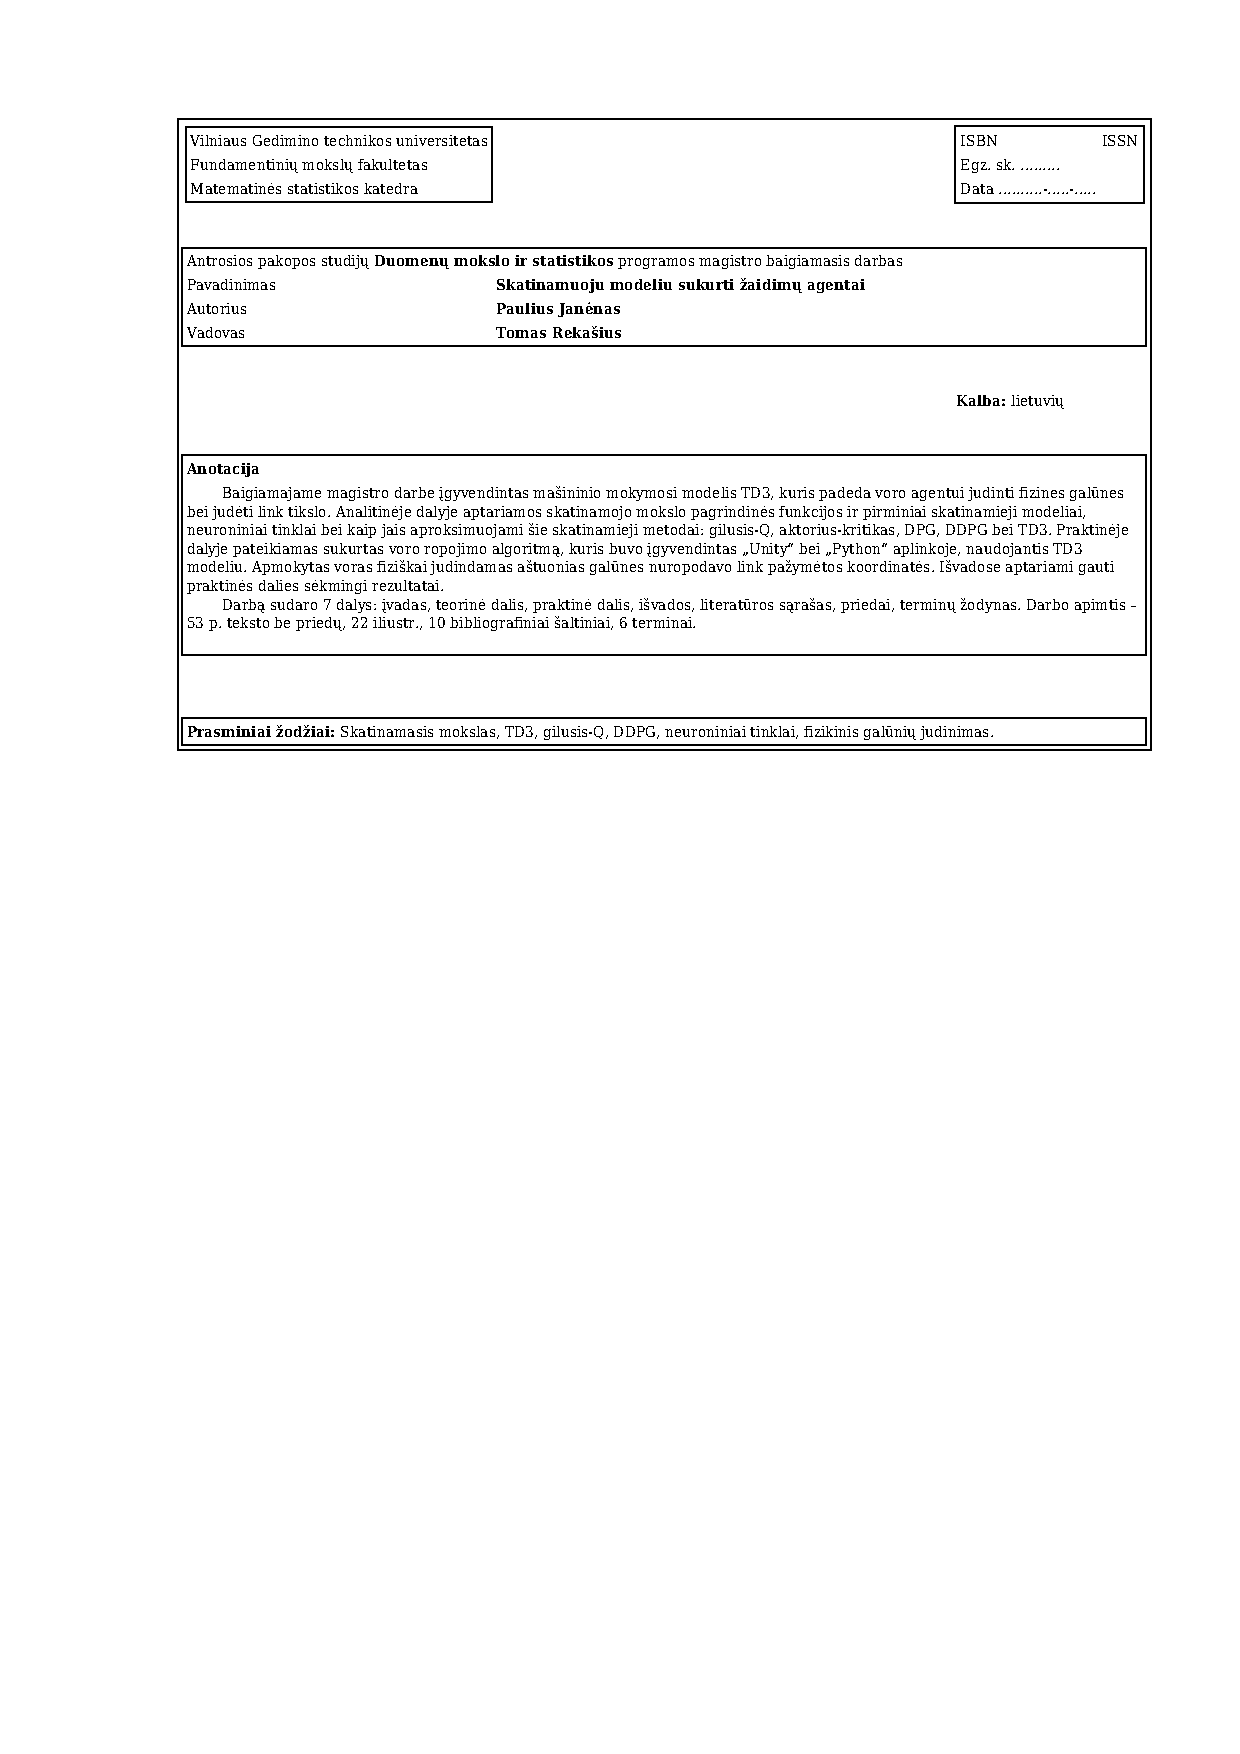
\includepdf[pages=-]{annotation_lt.pdf}
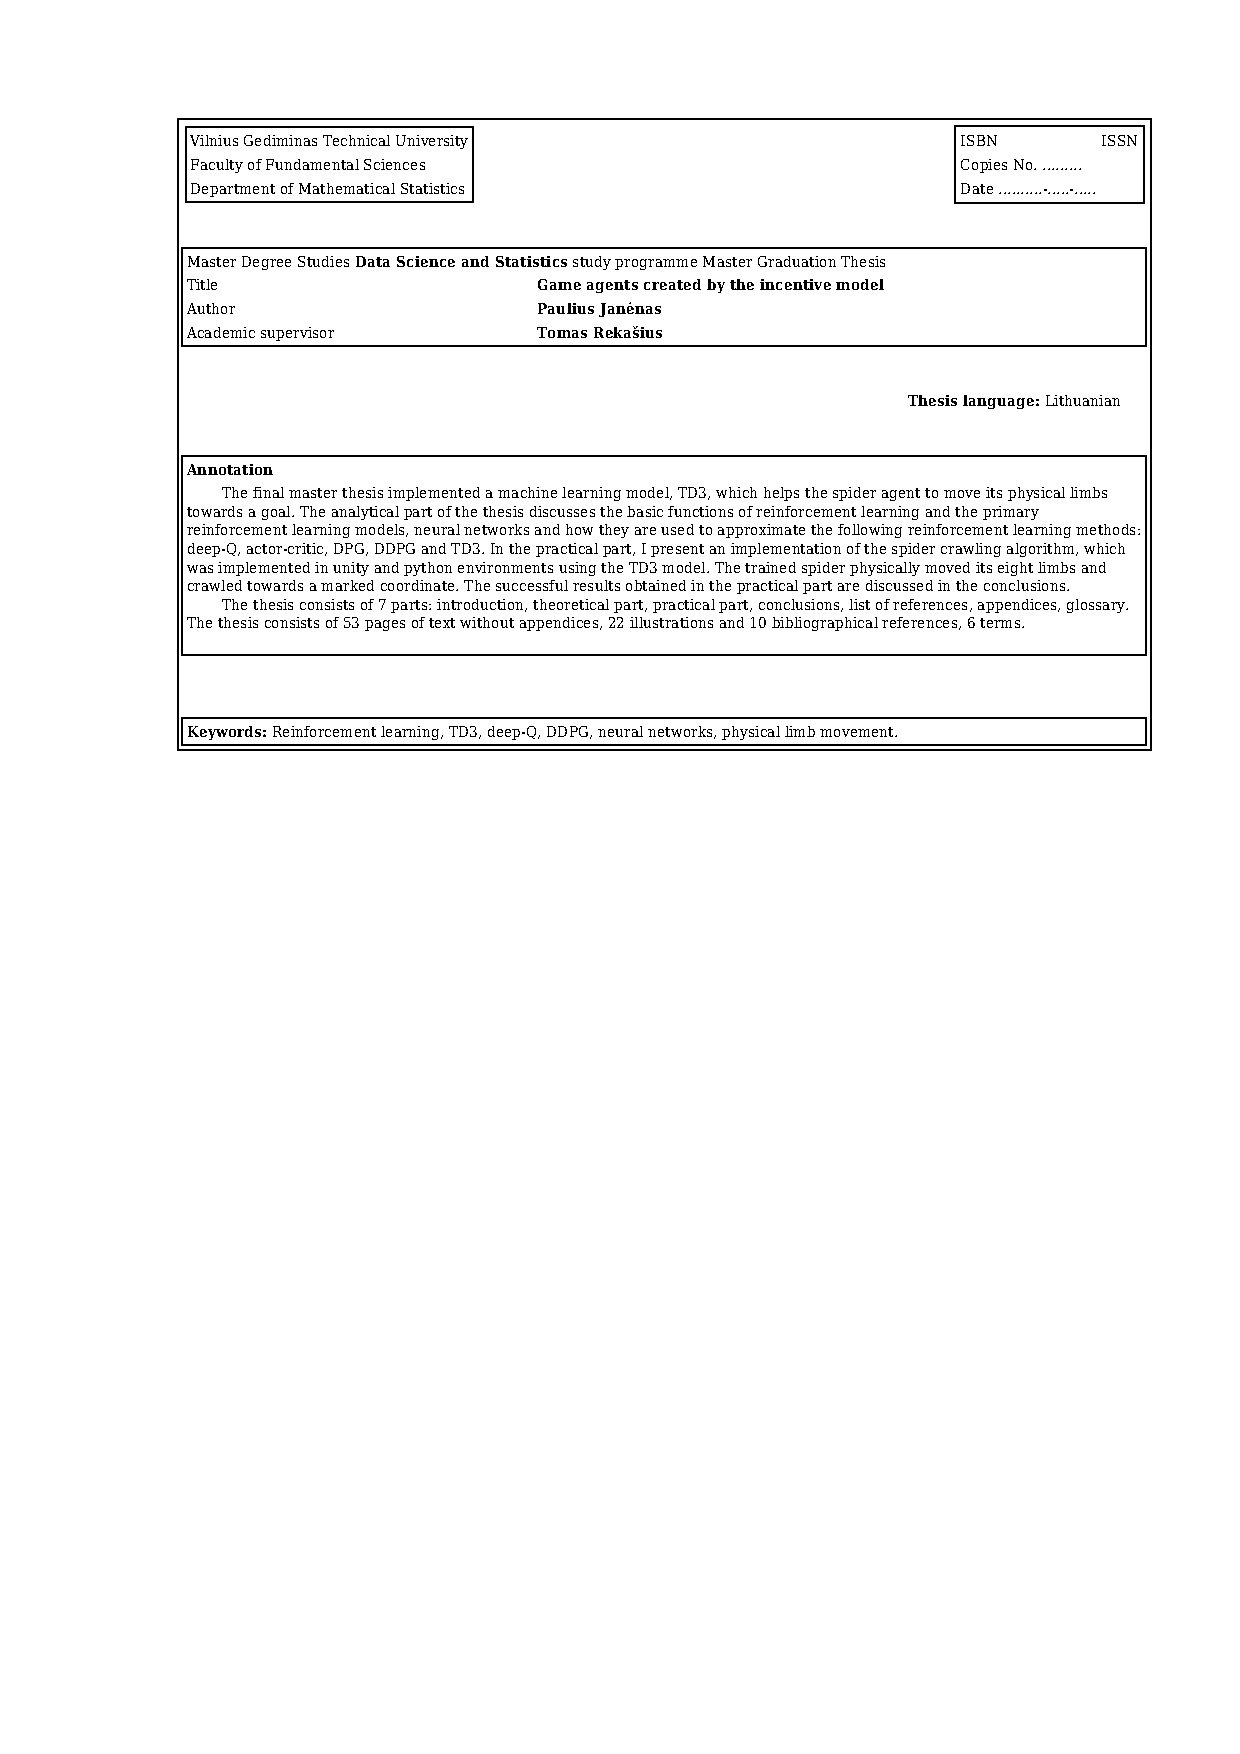
\includepdf[pages=-]{annotation_en.pdf}

% ------------------------------------------------------------------- TURINYS --
\tableofcontents
\newpage

\cleardoublepage
\phantomsection
\addcontentsline{toc}{section}{\listfigurename}
\listoffigures
\newpage

%\cleardoublepage
%\phantomsection
%\addcontentsline{toc}{section}{\listtablename}
%\listoftables
%\newpage


%\cleardoublepage
%\phantomsection
%\printglossaries
%\addcontentsline{toc}{section}{\listtablename}
%\listoftables
%\newpage

% -------------------------------------------------------------------- ĮVADAS --
\section*{Įvadas}
\phantomsection
\addcontentsline{toc}{section}{Įvadas}
%
Šių laikų žaidimų industrijoje sukurti \gls{Zaidimo agentas}, kuris realistiškai reaguoja į aplinką, yra sudėtinga užduotis, reikalaujanti daug laiko bei pastangų. Taip pat neretai prie laiko kaštų prisideda ir tai, kad prieš kuriant žaidimo agentą tam reikia tinkamai paruošti aplinką – sukurti pagalbinius įrankius, leidžiančius padaryti programavimo procesą lengvesnį. Tačiau net įdėjus pastangų programuojant agentus rezultatai yra dažnai prasti, jie nėra pakankamai protingi, žaidėjui nėra didžiulio iššūkio juos įveikti. Tai priveda prie didžiausio žaidėjų nepasitenkinimo – agentų sukčiavimo. Norint agentus padaryti protingesniais, jiems suteikiama žaidimo informacija, kuri yra neprieinama įprastiems žaidėjams. 

Per pastarąjį dešimtmetį įvykus neuroninių tinklų proveržiui buvo dedama daug vilčių, kad jie sugebės sukurti protingesnius žaidimo agentus. Tačiau neuroniai tinklai tėra funkcijos aproksimacijos metodas ir sunkiausia šio iššūkio dalis greitai atsiskleidė – kaip sukurti funkciją, kuri padėtų agentams tobulėti, tapti protingesniems? Šis klausimas buvo nagrinėtas per pastaruosius 70 metų, įtraukiant tokias mokslo šakas kaip dinaminis programavimas, Markovo modeliai, neuromokslai. Atradimai minėtose šakose privedė prie skatinamojo mokslo gimimo, kuomet 1987 metais šio mokslo pradininkai Sutton, R. bei Barto, A. moksliniame straipsnyje \cite{TDSutton} pirmieji sukūrė optimizavimo funkciją, pavadinta TD, padedančia agentams mokytis iš praeities rezultatų, siekiant pasirinkti tokius ateities veiksmus, kurie pagerintų ateities rezultatą. Funkcijos principas remiasi skatinimo metodais, kaip siunčiant paskatinimo impulsus agentui, jei jis atliko teisinga veiksmą, bei nubaudžiamas jei atliko neteisingą veiksmą. Tokiu principu agentas sukuria pozityvias bei negatyvias asociacijas su galimais veiksmais, kuriuos jis gali atlikti. Šį principą puikiai iliustruoja Pavlovo šunų eksperimentas \cite{Pavlov}. Sekančius dešimtmečius sekė šios funkcijos gerinimas, optimizavimas, bandymas išspręsti didelės dimensijos problemą – kuo didesnė būsenos ervės dimensija, tuo ilgiau užtrunka skaičiavimai. Ši problema buvo išspręsta pasitelkiant neuroninius tinklus, kurie aproksimuodavo TD funkciją. Šio metodo kulminacija įvyko 2016 metais, kuomet Google AlphaGo sugebėjo įveikti stalo žaidimą Go, kurio nesugebėjo įveikti nei viena komanda prieš tai dirbusi prie pirmųjų algoritmų, įveikusių šachmatų čempionus. Šiuo metu skatinamieji metodai aprėpia daugybe sričių: automobilių autonominis vairavimas, logistikos grandžių optimizavimas, robotikos judėjimo problemos ir dar daugybe kitų sričių. 

Šiame darbe bus išanalizuojamas skatinamasis mokymasis bei įgyvendintas vienas iš šio mokslo metodų - TD3. Teorinėje dalyje bus analizuojama šio metodo veikimo principai. Tai atlikus praktinėje dalyje šis metodas bus pritaikytas išspręsti roboto-voro fizinio judėjimo aplinkoje problemą.

%
\paragraph{Darbo aktualumas.} Dirbtiniui intelektui sugebėjus įveikti šachmatų čempionus buvo manoma, kad žmonių dominavimas tradiciniuose stalo žaidimuose pasibaigė. Tačiau programuotojų ambicijos išblėso, kuomet min-max paremti šachmatų algoritmai nesugebėjo įveikti kiniečių tradicinio stalo žaidimo – Go. To pagrindinė priežastis – neapskaičiuojamai didelė žaidimo būsenų erdvė. Kompiuteriai užtrukdavo per ilgai planuoti ėjimus ir jam neužtekdavo atminties išanalizuoti visus galimus ėjimus. Todėl iki šiol šis stalo žaidimas buvo neįveikiamas iki kol Google korporacija išleido skatinamojo mokymosi paremto algoritmo, kuris 2016 metais sugebėjo įveikti šių laikų geriausią Go žaidėją. Nuo to laiko skatinamųjų mokymosi metodų aktualumas vis labiau plito įtraukiant sritis kaip autonominiai automobiliai, robotika, finansai bei vis naujai populiarėjanti sritis – žaidimų industrija. 
%
\paragraph{Darbo tikslas.} Pritaikyti TD3 skatinamojo mokymosi modelį, kuris apmokytų simuliuojamą vorą vaikščioti 3D aplinkoje.
%
\paragraph{Uždaviniai.}
%
\begin{enumerate}
  \addtolength{\itemsep}{-0.5\baselineskip} 
  \item Išanalizuoti gilių neuroninių tinklų struktūrą.
  \item Įgyvendinti „Python“ bei „Unity“ duomenų sinchronizaciją.
  \item Išanalizuoti skatinamojo mokymosi modelio principus.
  \item Išanalizuoti Belmano, Q-mokymosi, TD funkcijas.
  \item Sukurti „Unity“ voro aplinką bei agentą, kuris bus apmokomas vaikščioti.
  \item Įgyvendinti TD3 mokymosi modelį bei apmokyti vorą vaikščioti sukurtoje aplinkoje.
\end{enumerate}


%
%
\newpage



% ------------------------------------------------------------------- SKYRIUS --
\section{Teorinė dalis}
%

Skatinamojo mokymo metodai remiasi neuroninių tinklų aproksimacijom, kurie bus nagrinėjami tolimesniuose skyriuose. Taigi šioje darbo dalyje nagrinėsiu giliųjų neuroninių tinklų veikimo principus. Tai atlikęs toliau nagrinėsiu skatinamojo mokymosi metodus bei kaip neuroniniai tinklai padeda juos įgyvendinti. Pagrindinis nagrinėjamas skatinamojo mokymosi modelis bus TD3. Tai yra modelis, kuris padeda agentui tolydžioje aplinkoje pasirinkti veiksmus, kurie suteikia didžiausią apdovanojimą. 


%
\subsection{Neuroninio tinklo struktūra}
%

Neuroninių tinklų sandarą galimą žiūrėti kaip į logistinės regresijos logistinių funkcijų veikimą. Kitaip tariant vieną neuroną galima traktuoti kaip logistinę funkciją, kuri išsiskaido į dvi dalis: tiesinę bei aktyvacinę. Tiesinėje dalyje suskaičiuojame tiesinę funkciją ir ją įvedame į aktyvacijos funkciją, kuri logistinėje regresijoje yra sigmoido funkcija. Tai yra identiška logistinei regresijai. Aktyvacinės funkcijos gali būti skirtingos, nebūtinai sigmoido. Pagrindinė skirtingų aktyvacinių funkcijų priežastis yra spartesnė svorių konvergacija į optimalią reikšmę. Dažnai naudojama Relu aktyvacinė funkcija \ref{eqn:Relu}, kuri neturi sigmoido nykstančio gradiento problemos, aptariamos \ref{Gradiento sprogimas} skyriuje. Ši problema pasireiškia kuomet sigmoido funkcijos reikšmė yra labai didelė arba maža, tuomet gradientas tampa beveik nulinis ir mokymosi procesas sustoja. 

\begin{equation}
\label{eqn:Relu}
f(x) = x = max(0,x)
\end{equation}

Pats neuroninis tinklas susideda iš logistinių funkcijų (jei naudojame ne sigmoid aktyvacinę funkciją tai jau nebėra logistinė funkcija) sluoksnių, kurie prasideda įvesties sluoksniu, viduryje paslėptuoju sluoksniu ir galiausiai išvesties sluoksniu. Visi klasifikatoriai turi vieną bendrą panašumą – įvesties bei paslėptuosius sluoksnius. Tačiau priklausomai nuo to ar atsakas yra klasifikacinis ar regresinis, kinta išvesties sluoksnis. 

Kuriant „Python“ aplinkoje neuroninius tinklus buvo pasitelkta vektorizacija, kuomet neuroninio tinklo įvestis nėra vienas stebinys, bet stebinių matrica. Visas įvestis, svorius, išvestis išsireiškus matriciniu pavidalu gaunamas ryškus neuroninių tinklų paspartėjimas. Neuroninio tinklo bendra naudota struktūra yra pateikta \ref{neuronu diagrama} paveikslėlyje.

\begin{figure}[h]
\centering
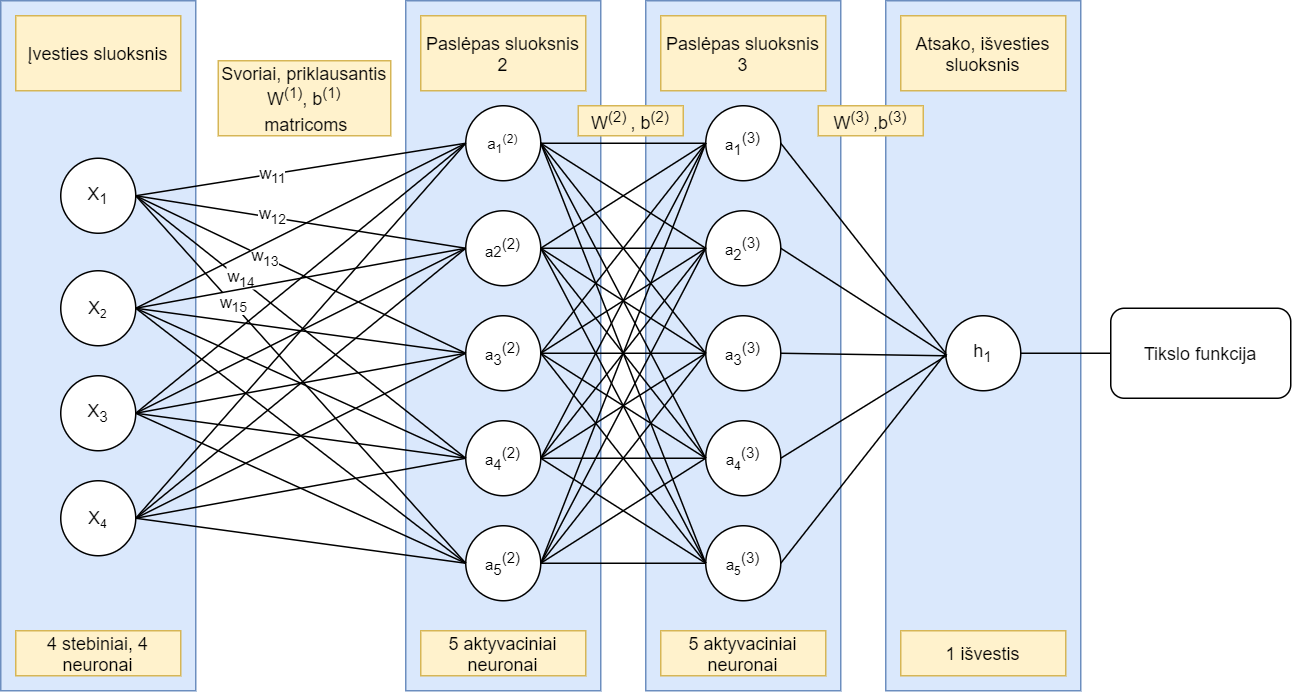
\includegraphics[width=1\textwidth]{neuronu diagrama}
\caption{Gilaus neuroninio tinklo bendra struktūra}
\label{neuronu diagrama}
\end{figure}

Vieno sluoksnio įvesties transformacijos vektorizaciją yra taip skaičiuojama:

$$
Z^{l}=W^{{l}^T} \cdot A^{l-1}+b^{l}
$$

Žymėjimas: $A^l$ yra $l$ sluoksnio neuronų reikšmės (matrica, kuri susideda iš $a^l \in \mathcal{R}^n$ elementų), kurias aktyvacinės funkcijos pateike (jei $l$ yra lygus įvesties sluoksniui, tai $A^l$ tampa duomenų įvesties vektorius $X$), o $W^{l^T}$ yra $l$ sluoksnio svoriai.
Šios transformacijos matricos eilutės yra skirtingų neuronų tiesinės transformacijos reikšmės, o stulpeliai žymi skirtingus mokymosi duomenis. Šią transformaciją įkėlus į aktyvacijos funkciją gauname galutinę perceptrono reikšmę.
Norint, kad neuroninis tinklas būtų tikslus, mes turime optimizuoti svorius. Tam pasitelkiame gradientinį nuolydį. Gradientinis nuolydis padeda surasti svorius, su kuriais tikslo funkcija įgyja mažiausią paklaidą. Tikslo funkcija sudaro tolygų paviršių, kurio skirtingos ašys yra svorių reikšmės bei viena iš jų yra tikslo funkcijos rezultatas. Pateiktame \ref{gradientinis nuolydis} paveikslėlyje apatinės ašis $x$ bei $y$ galima traktuoti kaip svorius, o viršutinę ašį kaip tikslo funkcijos paklaidą. 

\begin{figure}[h]
\centering
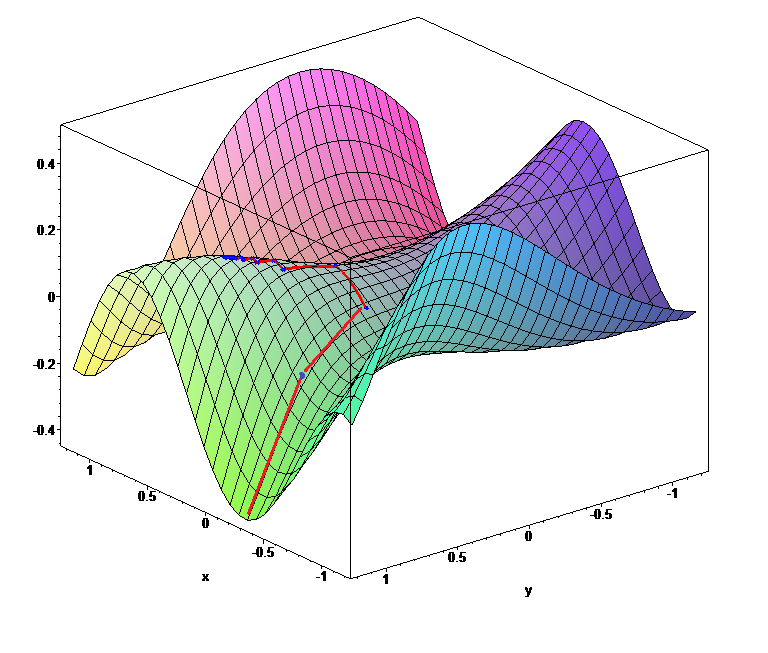
\includegraphics[width=0.7\textwidth]{gradientinis nuolydis}
\caption{Gradientinio nuolydžio pavyzdys}
\label{gradientinis nuolydis}
\end{figure}

Judindami svorius priešingą gradiento puse, mes judame ties tokiais svoriais, kurie mažina tikslo funkcijos paklaidą. Šią trajektoriją atspindi \ref{gradientinis nuolydis} paveikslėlyje esanti raudona kreivė, kuri kiekvienos iteracijos metu (mėlyni taškai) po truputi slenka žemyn, optimizuoja svorius.

Vėlgi gradientinio nuolydžio vektorizacija yra tokia pati tiek įvesties, tiek paslėptuose sluoksniuose, bet priklausomai nuo analizuojamos problemos - skirtinga išvesties sluoksnyje. Gradiento vektorizacija:

\begin{equation}
\label{eqn:backpropdz}
d Z^{l}=W^{l+1^{T}} d Z^{l+1} \cdot g^{l}\left(Z^{l}\right).
\end{equation}

Žymėjimas: $g^l(Z^l)$ yra dabartinio sluoksnio aktyvacinės funkcijos išvestinė. Ji yra sudauginama su visais matricos nariais. Gavus perceptronų išvestines $dZ^l$ galime toliau gauti svorių gradientus:


\begin{equation}
\label{eqn:backprop}
\begin{gathered}
d W^{l}=\frac{1}{m} d Z^{l} A^{(l-1)^{T}} \\
d b^{l}=\frac{1}{m}\left(d Z^{l} \text { matricos stulpeliu susumavimas }\right)
\end{gathered}
\end{equation}



Žymėjimas: stulpelių skaičius arba mokymosi duomenų kiekis yra žymimas $m$. Toliau bus aptariamos priekinė, atgalinė sklaida bei tikslo funkcijos, kurios sudaromos atitinkamai pagal turima klasifikacijos problemą.

%
\subsubsection{Neuroninio tinklo apmokymas taikant tiesioginio sklidimo algoritmą}
%

Įgyvendinti gilaus neuroninio tinklo struktūra pasirinktoje programavimo kalboje nėra sunku, kuomet pastebimas visiems sluoksniams bendras pasikartojantis skaičiavimo bruožas. Skaičiuojant tiesioginį sklidimą (judame neuroniniu tinklu iš kairės į dešinė) į neuroninį tinklą galima žiūrėti kaip į atskirus blokus susidedančius iš įvesties bei išvesties, kaip tai matosi \ref{forwardProp} paveikslėlyje.
\clearpage
\begin{figure}[h]
\centering
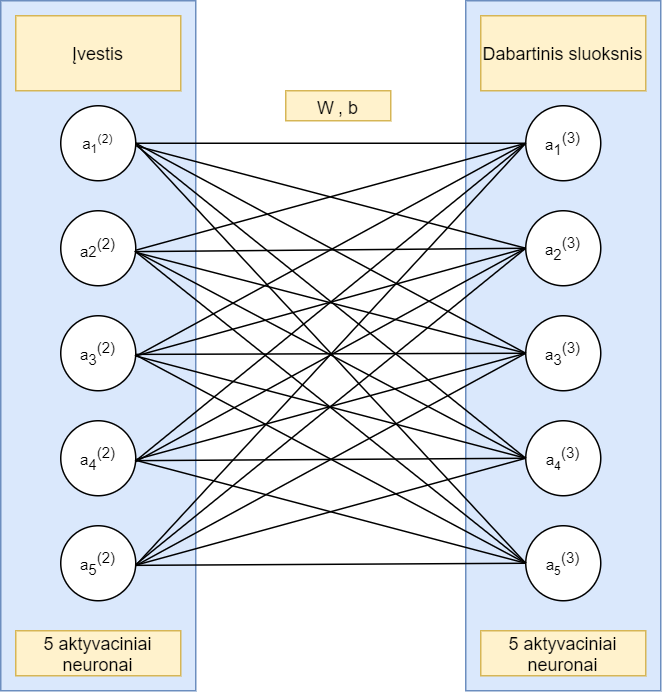
\includegraphics[width=0.6\textwidth]{ForwardProp}
\caption{Priekinio sklidimo vieno neuroninio sluoksnio apskaičiavimo grafas}
\label{forwardProp}
\end{figure}

Tokia forma išskaidžius neuroninį tinklą, jį tampa labai paprasta apskaičiuoti, tereikia iteruoti kiekvienu sluoksniu iš kairės į dešinę. Kiekvienos iteracijos metu praeitą sluoksnį traktuojame kaip įvesties sluoksnį ir naudodamiesi \ref{eqn:backprop} formulėmis apskaičiuojame dabartinio sluoksnio aktyvacinius neuronus. Šios operacijos metu svarbu išsaugoti tarpinius skaičiavimus, kaip tiesinės funkcijos bei aktyvacinę funkcijos apskaičiavimo rezultatą. Jos bus reikalingos apskaičiuoti gradientinį nuolydį, kaip tai matosi \ref{eqn:backpropdz} bei \ref{eqn:backprop} formulėse. Paskutinės iteracijos metu, atlikus aktyvacinės funkcijos apskaičiavimą, lieka tik apskaičiuoti tikslo funkcijos rezultatą. 
Šį struktūra pasižymi formulių universalumu, jos tinka neuroniniams tinklams, kurie yra negilieji bei gilieji, kitaip tariant - nepriklauso nuo sluoksnių kiekio. Atlikus tiesioginį sklidimą ir suskaičiavus tikslo funkcijos klaidą, galime pradėti ją mažinti, judėdami priešinga gradiento linkme. Tai atliekama įgyvendinant atgalinio sklidimo metodą.
	

%
\subsubsection{Neuroninio tinklo atgalinio sklidimo algoritmas}
%

Atgalinės sklaidos struktūra yra vos ne identiška priekiniai sklaidai. Pagrindiniai skirtumai yra sukeistos vietos apskaičiuojamo sluoksnio bei įvesties sluoksnio. Tačiau kaip ir priekinės propogacijos atveju, mes atliekame panašias iteracijas, tik šį kart pradedam nuo tikslo funkcijos ir judame link pirmo sluoksnio, iš kairės į dešinę. Atliekant šias svorių atnaujinimo operacijas, kaip tai matosi \ref{eqn:backpropdz} bei \ref{eqn:backprop} formulėse, pasitelkiame priekinės sklaidos metu išsaugotais duomenimis. 

\begin{figure}[h]
\centering
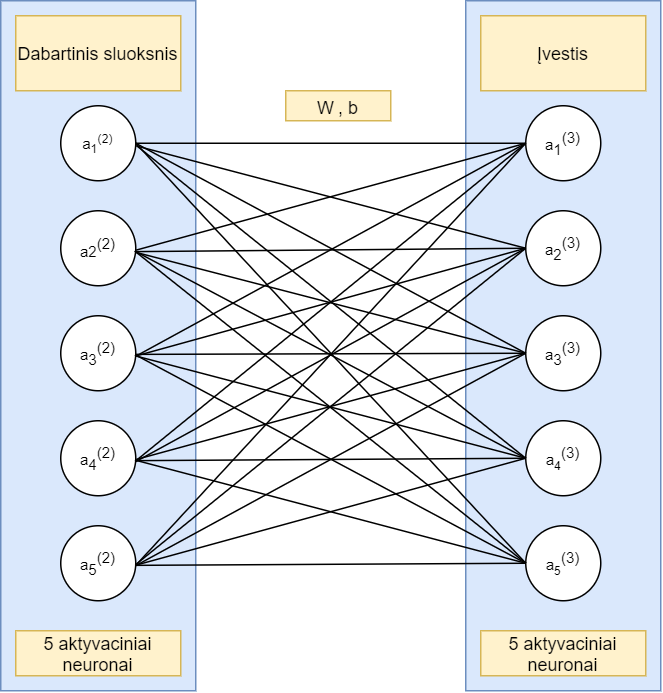
\includegraphics[width=0.6\textwidth]{BackProp neuronais}
\caption{Atgalinio sklidimo vieno neuroninio sluoksnio apskaičiavimo grafas}
\label{BackProp neuronais}
\end{figure}

%
\subsection{Neuroninių tinklų klasifikatorių tipai}
%

%
\subsubsection{Binarinis klasifikatorius}
%

Tai klasifikatorius, kuris vos ne identiškas logistinei regresijai. Klasifikuoja binarinius atsakus. Išvesties sluoksnis turi tik vieną neuroną bei jo reikšmės transformacija sutampa su logistinės regresijos logtikėtinumo funkcija:

\begin{equation}
\log (L)=\ell=\sum_{i=1}^{n}\left[y_{i} \log \left(p_{i}\right)+\left(1-y_{i}\right) \log \left(1-p_{i}\right)\right].
\end{equation}

Šios funkcijos gradientas susiprastina į šią formą:

\begin{equation}
d Z^{l}=A^{l}-Y,
\end{equation}

kur $l$ yra paskutinis sluoksnis, $Y$ yra tikroji atsako reikšmės, o $A^l$ yra neuroninio tinklo gauti atsakai. Turint $dZ^l$ galima gauti svorių gradientus bei neuronų gradientus, kaip tai buvo parodyta prieš tai buvusiuose skyriuose. Turint svorių gradientus atnaujiname svorius:

\begin{equation}
W^{l}=W^{l}-\alpha dW^{l},
\end{equation}

kur $\alpha$ nurodo gradientinio žingsnio dydį.

%
\subsubsection{Daugiau nei viena klasė}
%

Klasifikuojant daugiau nei vieną klasę yra naudojamas entropijos tikslo funkcija. Tikslo funkcijos forma:

\begin{equation}
L(y, \hat{y})=-\sum_{i=1}^{N} y_i \cdot \log (\hat{y_i}),
\end{equation}
kur $y$ yra tikroji reikšmė, o $\hat{y}$ yra aproksimuota.


Kuomet paskutinio sluoksnio aktyvacinė funkcija yra „soft-max“:
\begin{equation}
\label{eqn:softmax}
\sigma(z_i) = \frac{e^{z_{i}}}{\sum_{j=1}^K e^{z_{j}}} \ \ \ kur \ i=1,2,\dots,K,
\end{equation}

šios funkcijos gradientas labai gražiai susiprastina ir paskutinio sluoksnio gradientas atrodo ši taip:

\begin{equation}
d Z^{l} = (Y- \hat{Y})
\end{equation}

kur $l$ yra paskutinio sluoksnio indeksas, o dydžioji $Y$ yra vektorizacija daugybės stebinių į vieną matricą.

Iš šio gradiento galime seniau aptartais metodais gauti $W$ bei $b$ gradiento reikšmes. Galima naudoti ir mažiausių kvadratų metodą, tačiau gradientinis nuolydis konverguotų lėčiau.
Taip pat pagrindinis skirtumas tarp binarinio klasifikatoriaus yra aktyvacinė funkcija. Šį kart tai nėra sigmoido funkcija, o „soft-max“ normalizacija, kuomet gautos eksponentinės reikšmės konvertuojamos į tikimybių pasiskirstymą, kaip tai matosi \ref{eqn:softmax} formulėje. Taigi šis metodas yra dažnai naudojamas klasifikuoti reikšmes, kurios turi daugiau nei vieną klasę.

%
\subsubsection{Tiesinės regresijos atsakas}
%

Jei atsakas yra regresinis, tuomet tikslo funkcija tampa didžiausių kvadratų optimizacija ir paskutinis neuronas neturi aktyvacijos funkcijos. Tikslo funkcijos mažiausių kvadratų sumos vidurkio formulė:

\begin{equation}
MSE=\frac{1}{N} \sum_{i=1}^{N}\left(y_i-\hat{y_i}\right)^{2}
\end{equation}
kur $y$ yra tikroji reikšmė, o $\hat{y}$ yra aproksimuota.

Neuroniniai tinklai su regresine tikslo funkcija yra puikus agentų apmokymo pavyzdys, įrodantis kad priklausomai nuo užduoties, nebūtina imtis sudėtingų skatinamojo mokymosi metodų, norint sukurti protingą agentą. Su šiuo metodu buvo optimizuojamas stalo teniso žaidimas, kuriame atsakas buvo stalo teniso raketės pozicijos optimali padėtis atmušti atskriejanti kamuoliuką, kaip tai matosi \ref{pingpong} paveikslėlyje. Tai buvo paprastas gilus neuroninis tinklas su dvejais paslėptais sluoksniais po 12 neuronų. Buvo pasitelktas stochastinis gradientinis nuolydis, kuomet kiekvieno žaidimo kadro metu buvo nusiunčiami neuroniniam tinklui dabartinės raketės padėtis bei kamuoliuko trajektorija. Šiam uždaviniui neuroninio tinklo nereikia, pakaktu paprasto algoritmo ar tiesinės regresijos, tačiau tai gerai iliustruoja jo veikimo principus. Pradžioje raketės juda padrikai, bet bėgant laikui, vykstant gradientiniui apmokymui, rakečių judėjimas vis tikslėja.

\begin{figure}[h]
\centering
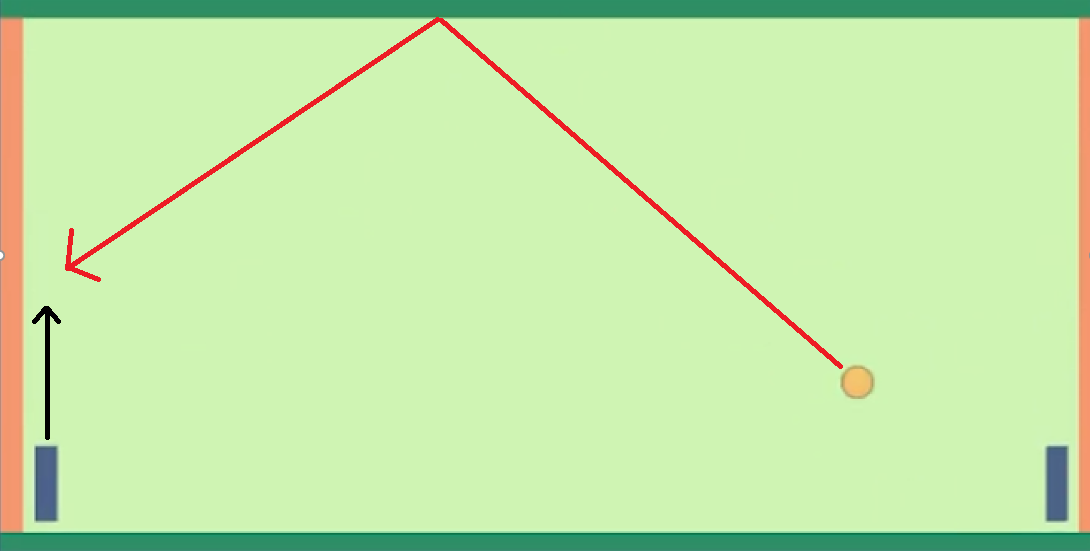
\includegraphics[width=1\textwidth]{pingpong}
\caption{Sukonstruota stalo teniso simuliacija}
\label{pingpong}
\end{figure}

\ref{pingpong} Paveikslėlyje raudona trajektoriją yra neuroninio tinklo įvestis, apskaičiuojanti kamuoliuko galutinę padėtį. Juoda trajektorija yra neuroninio tinklo išvestis, raketės greičio vektorius, simbolizuojantis pozicija, kurioje raketė turi atsirasti

%
\subsubsection{Tiesinė regresija su daugybe atsako kintamųjų}
%

Identiška tiesinės regresijos funkcijai, tačiau šiuo atveju paskutinis sluoksnis turi daugiau nei vieną neuroną. Tuomet tikslo funkcija atrodo šitaip:

\begin{equation}
L=\frac{1}{m * 2} * \sum\left(Z^{l}-Y\right)^{2}
\end{equation}

Vektorizacija identiška tiesinės regresijos atveju, tik atsako kintamasis Y turi ne vieną eilutę, o daugiau. Eilutės žymi pasirinkto sluoksnio neuronų reikšmes.
Su šiuo metodu buvo optimizuotas automobilio kontroleris, kurio tikslas buvo apvažiuoti trasą. Įvestis buvo normalizuota automobilio sensorių informacija, kurie pateikdavo trasos barjero atstumą. Išvestis buvo automobilio stabdymo ir greičio pedalo stiprumai bei vairo pozicija. Apmokius neuroninį tinklą rezultatai buvo tragiški, automobilis važiuodavo tik tiesiai. Tačiau pritaikius Adamo metodo gradientinį nuolydį ir taip sumažinus modelio klaidą, buvo pasiekti tenkinami rezultatai. Automobilis sugebėdavo apvažiuoti trasą. 

%
\subsection{Neuroninių tinklų reguliarizacija}
%

Neuroninių tinklų reguliarizacija reikalinga norint išvengti modelio prisitaikymo prie mokymosi duomenų. Ji padeda pagerinti testavimo duomenų tikslumą. Toliau nagrinėsiu metodus, kurie tai padeda pasiekti.

%
\subsubsection{L1 bei L2 reguliarizacija}
%

Didžiuliai neuroninio tinklo svoriai retai gerai generalizuoja modelį, jie numuša testavimo imties tikslumą. Todėl svarbu neleisti svoriams tapti milžiniškais. L1 bei L2 reguliarizacija tai padeda pasiekti. Prie tikslo funkcijos lygties mes pridedame Lagrandžo svorių apribojimus, L2 atveju formulė išsireiškia tokiu pavidalu:

\begin{equation}
\label{JFunkcija}
J(W, b, X, y)=\frac{1}{m} \sum L(y, \hat{y})+\frac{\lambda}{2 * m} \sum\left\|w^{l}\right\|^{2},
\end{equation}
kur $\lambda$ yra lagrandžo daugiklis ir taip pat hiperparametras.

Matome, kad prie pagrindinės tikslo funkcijos prisideda papildoma bauda. Kuo didesni svoriai, tuo didesnė bauda. L1 atveju mes vietoj ilgio kvadrato, naudojame absoliutinę reikšmę. L2 skiriasi nuo L1 tuo, kad L2 padeda tuos svorius paversti nuliais, kurie turi mažai įtakos gradientiniam nuolydžiui, kaip tai matosi \ref{regularization} paveikslėlyje. Tačiau abejais atvejais mes nepasieksime optimalios reikšmės ir išmainysime dispersiją į prisitaikyma (bias), taip pasiekdami tikslesnį testavimo duomenų klasifikavimą, jei modelis yra per daug prisitaikęs prie mokymo duomenų.
Gradientą šiai funkcijai lengva surasti, kadangi matome, kad \ref{JFunkcija} funkcija išsiskaido į dvi dalis. Telieka surasti išvestines L2 formai, kas yra labai paprasta.

\begin{figure}[h]
\centering
\includegraphics[width=1\textwidth]{regularization}
\caption{Reguliarizacija - kairėje L1, dešinėje L2}
\label{regularization}
\end{figure}

%
\subsubsection{Atvirkštinis išmetimas}
%
Šio metodo esmė, išjunginėti kiekvieno sluoksnio neuronus su tam tikra tikimybe. Juos išjungus, kiti neuronai turės perimti jų darbą. Tai padeda išvengti atveju, kuomet vienas neuronas persimoko. Tačiau išmetimo atveju vidutiniškai neuronų išvestis sumažėja išmetimo tikimybės procentu. Todėl atvirkštiniu išmetimu, mes po išmetimo operacijos kiekvieną neurono $Z$ reikšmę padaliname iš išmetimo tikimybės taip padidindami neurono išvestį ir gražindami to sluoksnio tikėtiną reikšmę į prieš išmetimą buvusią.



%
\subsubsection{Duomenų augmentacija}
%

Šis metodas taikomas, kuomet neturime pakankamai duomenų apmokymui, ko neuroniniams tinklams reikia nepaprastai daug. Jei duomenys susideda iš nuotraukų, tuomet augmentacijos metu mes galime nuotraukas apsukti, priartinti, karpyti ir panašius metodus taikyti, norint padidinti mokymosi duomenų imti.

%
\subsubsection{Įvesties normalizacija}
%

Gradientinio nuolydžio konvergacijos greitis priklauso nuo paviršiaus išsidėstymo. Paviršius gali būti labai susispaudęs bei banguotas, kas neleidžia atlikti didžiulių gradientinių žingsnių. Tokiais atvejais dideli žingsniai, gali šokinėti aplink optimalią reikšmę bei tokiu būdu niekados nekonverguoti. Taip pat svoriai nėra proporcingai panašus, vieni turi žymiai didesnę įtaka nuolydžiui, kiti mažesne. Tokiu atveju paimti dideli gradiento žingsniai gali vėlgi nekonverguoti. Tačiau normalizavus įvesties duomenis, paviršius išsilygina bei yra lengviau optimizuoti. Normalizavimas paremtas paprasčiausiu statistiniu $Z$ normalizavimu. Jis atliekamas, kuomet įvesties duomenis pasižymi skirtingais duomenų intervalais – vienos įvesties intervalas [0,1], kitos [0,1000].

%
\subsection{Neuroninių tinklų parametrų inicializacija}
%


%
\subsubsection{Gradiento sprogimas bei nykimas, aktyvacinių funkcijų parametrų priskyrimas}
%
\label{Gradiento sprogimas}
Priekinės sklaidos neuroninio tinklo žingsnyje, kuomet skaičiuojame išvestį, galime pastebėti tokį neuroninio tinklo bruožą

\begin{equation}
\hat{y}=W^{l}  W^{l-1}  W^{l-2}  \ldots  X
\end{equation}

Matome, kad jei $W^l$ svorių parametrai priskiriami su didelėmis reikšmėmis, turint daugybe sluoksnių mūsų tiek neurono tiek svorių reikšmės ekponentiškai išaugs. Tuo tarpu jei parametro reikšmės $W^l$ priskiriamos su mažesnėms nei vieneto reikšmėm, svoriai greitai tampa nuliais. Norint to išvengti visų neurono sluoksnio aktyvacijų reikšmių vidurkis turi būti lygus nuliui bei variacija visuose sluoksniuose išlikti vienoda. Šių tikslų padeda pasiekti svorių priskyrimo metodai. Dažniausiai svoriai yra paimami iš $\mathcal{N}(0,1)\ast0.001$. Šie svoriai nėra blogi jei turime tik pora sluoksnių, tačiau didėjant sluoksniams, kaip matėme prieš tai, neuronų reikšmės taps nuliais. Todėl, priklausomai nuo sluoksnio aktyvacijos, naudojame specifinius metodus priskiriant svorius. Norint kad šie metodai veiktų, įvestis privalo būti normalizuojama $Z$-normavimo principu. 

\begin{enumerate}
  \addtolength{\itemsep}{-0.5\baselineskip} 
  \item 	Jei aktyvacijos funkcija yra $tanh(x) = \frac{e^x - e^{-x}}{e^x + e^{-x}} = \frac{1 - e^{-2x}}{1 + e^{-2x}}$, svoriai imami iš $\mathcal{N}(0,\frac{1}{n^{l-1}})$, kur n yra neuronų skaičius sluoksnyje, šiuo atveju tai būtų praeito sluoksnio neuronų skaičius.
  \item 	Jei aktyvacijos funkcija yra $Relu(z) = max(0, z)$, svoriai imami iš $\mathcal{N}(0,1)\ast\frac{2}{\sqrt n}$.
  \item 	Jei aktyvacijos funkcija yra sigmoidas $\sigma(z) = \frac{1} {1 + e^{-z}}$, svoriai imami iš $\frac{\mathcal{N}(n^{l-1},n^l)}{\sqrt n}$.
\end{enumerate}

%
\subsection{Mokymosi greičio didinimas }
%
Jei turime labai daug duomenų, matricų operacijos užima daug laiko. Todėl naudojame tolimesnius metodus, kurie paspartina mokymosi procesą.

%
\subsubsection{Mažos mokymosi imties metodas}
%

Metodo principas labai paprastas – iš visos duomenų imties paimame dalį skirstinio ir su šia gauta maža mokymosi imtimi apmokome modelį. Kiekviena tokia dalis negražins optimalaus gradiento vektoriaus, tačiau kadangi duomenis yra iš to pačio pasiskirstimo mes vis tiek judėsime į optimalias svorių reikšmes ir galiausiai konverguosime į optimalius svorius.

%
\subsubsection{Stochastinis nuolydis}
%

Beveik toks pats kaip praeitas metodas, tik dar ekstremalesnis atvejis – gradientas gaunamas iš vieno imties elemento, stulpelio. Vektorizacija šiuo atveju praranda visą savo greitį, taip pat gradiento vaikščiojimas neatrodo tolygus, juda vos ne į visas puses. Tačiau bendra gradientų krypties tendencija juda link tikslo funkcijos klaidos mažinimo. To priežastis yra išlieka tokia pati, kaip praeito metodo: kadangi duomuo yra iš to pačio pasiskirstimo mes vis tiek judėsime į optimalias svorių reikšmes. Šis metodas yra nuolatos taikomas skatinamuosiuose mokymosi metoduose.

%
\subsection{Gradientinio nuolydžio metodo optimizavimas}
%

Norint pasiekti greitesni svorių konvergavimą yra sukurta skirtingų gradientinio nuolydžio metodų, kurie netik pagreitina konvergaciją bet ir padeda kovoti su didelėmis gradiento problemomis – keliavimas plokščiu paviršiumi bei lokalus minimumai.

%
\subsubsection{Momentinis gradientinis nuolydis bei eksponentiškai pasvertų svorių vidurkis}
%

Pagrindinis šio optimizavimo principas remiasi momentiniu nuolydžiu, kuomet gradientas įgyja pagreiti ties dažniausiai pasikartojančiu vektoriumi. Primena įsibėgėjusį automobilį. Šis įsibėgėjimas padeda išvengti lokalių minimumu, kaip tai matosi \ref{momentinisGreitis} paveikslėlyje. Jame pavaizduoti skirtingi gradientinio mokymosi algoritmai, kurie pradeda tame pačiame taške bei kurių dauguma sustoja mokytis ties lokaliu minimumu. Tačiau momentinio mokymusi paremti gradientinio nuolydžio metodai praskrieja lokalųjį minimumą, kuris tik trumpam sumažina gradiento greitį. Taigi momentinio greičio intuicija labai paprasta: jei gauname nauja gradiento reikšmę, kuri nurodo judėti priešinga linkme, ji yra atsveriama gradieno įsibėgėjimo greičiu ir gradientas tik truputi sulėtėja. Šio gradiento formulė primena eksponentiškai pasvertų svorių vidurkio formulę ir išsireiškia tokiu pavidalu:

\begin{equation}
V d w=\beta_{1} \cdot V d w+\left(1-\beta_{1}\right) \cdot d w
\end{equation}

Kur $\beta_1$ yra parametras nuo 0 iki 1, dažniausiai būnantis 0.9. Kaip matome naujausi gradientai prie galutinės gradiento reikšmės prisidės tik $(1-\beta_1)$ dydžiu, kas suteikia momentinio greičio pavidalą. Šis pasvertų vidurkių principas yra plačiai naudojamas skatinamuosiuose mokymosi metoduose ir jį galima pastebėti visuose pagrindinėse formulėse. Skatinamuosiuose mokymosi metoduose šios formulės principą galima traktuoti kaip gradientinį nuolydį - po truputi konverguojame ties optimaliomis reikšmėmis.

\begin{figure}[h]
\centering
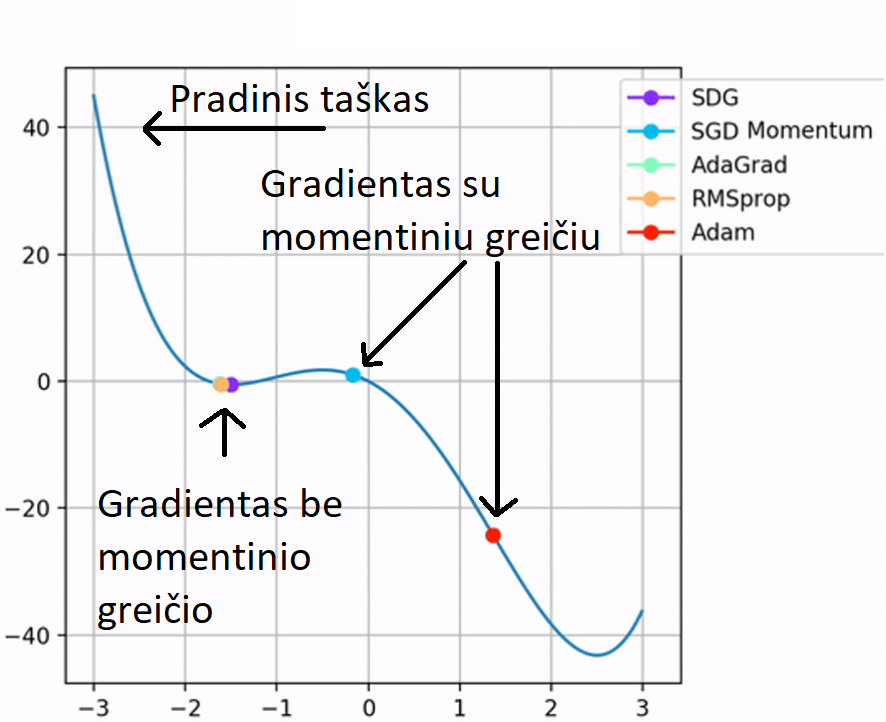
\includegraphics[width=.7\textwidth]{momentinisGreitis}
\caption{Gradientinė optimizacija su ir be momentinio greičio. SGD momentinis bei Adam konverguoja į globalų minimumą, kiti konvergavo į lokalų minimumą}
\label{momentinisGreitis}
\end{figure}

%
\subsubsection{RMSProp}
%

Tai gradientinio nuolydžio metodas, kurio tikslas pagreitinti gradientą, kuomet judame lygia plokštuma. Tačiau kaip matome iš \ref{momentinisGreitis} paveikslėlio RMSProp kenčia nuo momentinio greičio neturėjimo ir sustoja ties lokaliu minimumu. RMSProp forma labai panaši į momentinio gradiento:

\begin{equation}
S d w=\beta_{2} \cdot S d w+\left(1-\beta_{2}\right) \cdot (d w)^{2}.
\end{equation}

Svorių atnaujinimo formulė:

\begin{equation}
W=W-\alpha \frac{d w}{\sqrt{S d w}}
\end{equation}

Empiriškai galime pastebėti, kad didelės gradiento reikšmės sumažės, tačiau mažos padidės. Todėl šis metodas padeda išspręsti lėtą judėjimą lygumomis. Rekomenduojamas $\beta_2$ dydis yra 0.99.

%
\subsubsection{Adam}
%

Adam\cite{Adam} metodas yra vienas populiariausių gradientinio nuolydžio metodų. Jo tikslas sumažinti dvi problemas - lokalius minimumus bei judėjimas plokštuma. Tai pasiekiame sujungiant momentinį greitį bei RMSProp:

\begin{equation}
W=W-\alpha \frac{V d w}{\sqrt{S d w}}
\end{equation}

$Vdw$ suteikia momentinį greitį kiekvienam svoriui. Bet jei momentinis greitis yra didelis $Sdw$ jį sumažiną. Tačiau jei gradientas užstringa lygumoje, $Sdw$ padeda atstrigti.
Šį metodą pritaikiau minėtame automobilio kontrolerio pavyzdyje. Jis padėjo pasiekti trigubai mažesnį klaidos dydį ir taip pagerino automobilio kontrolerį.


%
\subsection{Skatinamasis mokymasis}
%

Skatinamojo mokymosi metodai yra mašininio mokymosi metodai, kurie apdovanoja pageidaujamus veiksmus bei baudžia nepageidautinus veiksmus. Naujuosiuose skatinamuosiuose modeliuose apdovanojimo bei baudos dydis tėra vienintelė informacija, kurią modelis težino. Jei tiesinėje regresijoje mes nuolatos turėdavome tikrąsias reikšmes, ties kuriomis bandėme pritaikyti modelį, šiuo atveju tokia informacija yra nepasiekiama. Todėl mūsų modelis turi nuolatos tyrinėti aplinką, kaupti naujas patirtis. Šiuos duomenis gauname iš aplinkoje esančio roboto ar agento, kuris duotoje aplinkoje stengiasi atlikti optimalius veiksmus ir pagal juos susidaryti geriausių siūlomų veiksmų modelį. 

Šią veiksmų eigą apibendrina bendrasis skatinamųjų modelių grafikas, pateiktas \ref{RLmodel} paveikslėlyje. Jis iliustruoja praktinės dalies pagrindinės užduoties įgyvendinimą, voro keturių galūnių judinimą, kuriomis bandoma kuo arčiau priartinti vorą ties žaliu kubeliu. 

\begin{figure}[h]
\centering
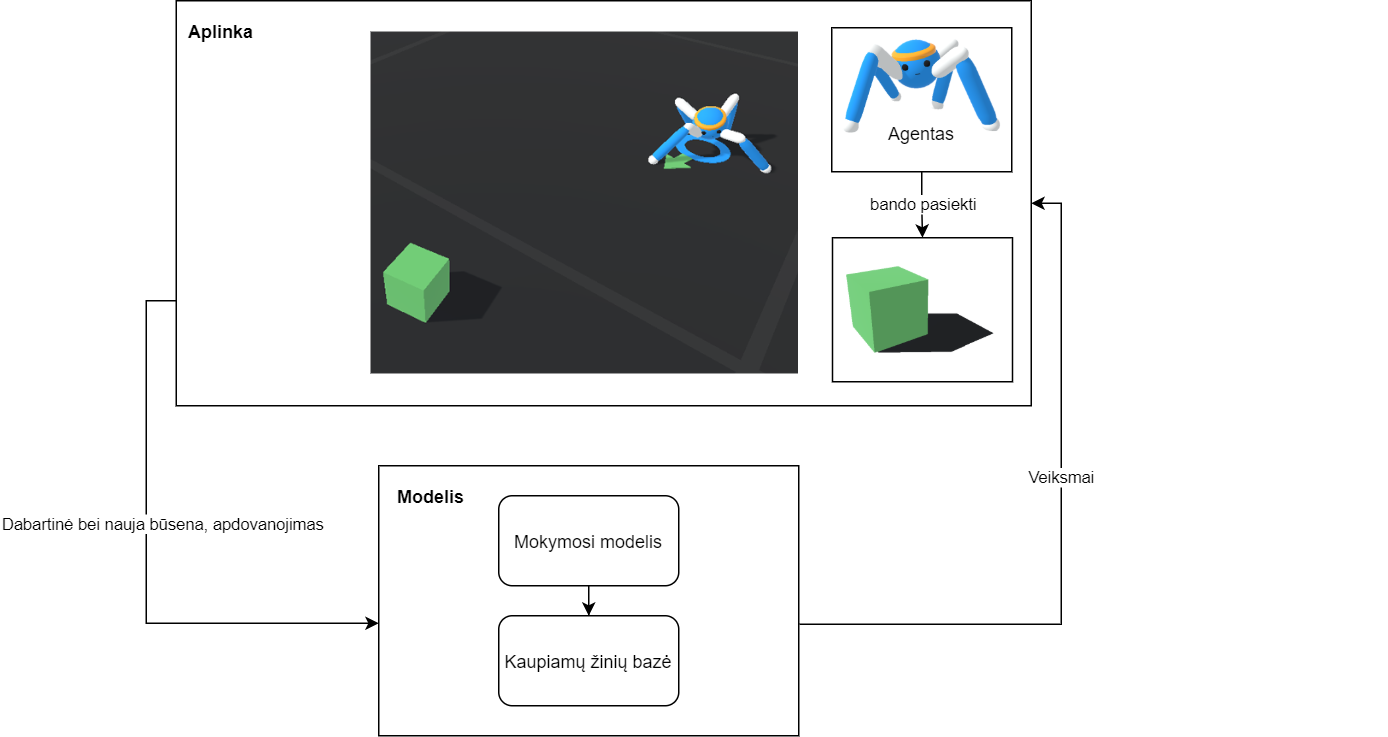
\includegraphics[width=1.3\textwidth]{RLmodel}
\caption{Bendras skatinamojo mokslo modelis}
\label{RLmodel}
\end{figure}



Šio modelio veikimo principai išsiskaido į šias dalis:
\begin{enumerate}
  \addtolength{\itemsep}{-0.5\baselineskip} 
  \item aplinka. 
  \item agentas. 
\end{enumerate}

\paragraph {Aplinka.}\mbox{}\\
Aplinkoje egzistuoja mūsų agentas, kuris priiminėja modelio sugeneruotus veiksmus. Pateiktame pavyzdyje tai būtų voro galūnių judėjimo trajektorijos. Atlikęs duotus veiksmus, voras įgauną naujas būsenas, pajuda į naują poziciją. Nauja įgyta būsena bei prieš tai buvusi, nusiunčiama modeliui. Taip pat modeliui nusiunčiame apdovanojimo dydį. Jis apskaičiuojamas naudojantis naujai sugeneruotos būsenos naudingumu. Naudojantis voro pavyzdžiu tai atitiktų voro greičio vektorio laipsnio sutapimu su norimos krypties vektoriumi, kaip tai matosi \ref{voroGreicioVektoriai} paveikslėlyje. Šiuo atveju apdovanojimas būtų nulinis, nes vektorių trajektorijos visai nesutampa. Atlikus veiksmą bei apskaičiavus jo naudingumą, tokiu būdu gaunamas ryšys tarp veiksmo, kuris sugeneruoja naują būseną, bei įgyto apdovanojimo, naujoje būsenoje. Šis ryšys tarp veiksmo bei gauto rezultato yra neseniai atgimusio skatinamojo mokslo pamatas, kuriuo moderniausi algoritmai ne per seniausiai pradėjo vadovautis, atradus apdovanojimų taisyklių gradientą bei pradėjus taikyti neuroninius tinklus. 

\paragraph {Agentas.}\mbox{}\\
Agento sluoksnis susideda iš mokymosi modelio bei žinių bazės, kurioje kaupiami gauti aplinkos rezultatai, susidedantis iš vektorių su šiomis reikšmėmis - praeita būsena, atliktas veiksmas, nauja būsena ir apdovanojimas. Mokymosi modelis naudojasi sukauptų žinių baze gerinti savo modelio rezultatus. Modelio tikslas yra pateikti tokias veiksmų sekas, kurios suteiktų didžiausią įmanoma apdovanojimą. Voro pavyzdžiu tai būtų sėkmingas žalio kubelio pasiekimas. Modelio apmokymui yra sukurta daugybe įvairių metodų ir šiame darbe bus nagrinėjamas vienas iš jų - TD3


\begin{figure}[h]
\centering
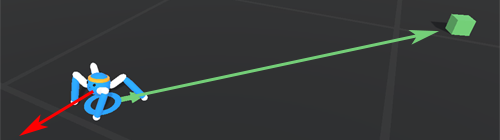
\includegraphics[width=1\textwidth]{voroGreicioVektoriai}
\caption{Apdovanojimo pavyzdys, pagal voro greičio (raudona rodyklė) bei norimo judėjimo (žalia rodyklė) vektorių atitikimu}
\label{voroGreicioVektoriai}
\end{figure}

Taigi visas skatinamasis mokslas paremtas tik vienu kintamuoju - apdovanojimo gausumu. Šis apdovanojimas apdovanoja pageidautiną elgesį bei baudžia už neigiamą elgesį. Tokiu būdu agentas skatinamas siekti didžiausio ilgalaikio nuopelno, kas veda į optimalų sprendimą. Tolimesniuose skyriuose bus aptariama kaip iš šio vieno kintamojo yra konstruojami visi skatinamojo mokslo modeliai.

%
\subsubsection{Skatinamojo mokslo pagrindiniai kintamieji, stacionariojo pasiskirstymo problema}
%

Kad ir kokį skatinamojo mokslo uždavinį spręstume, mes visados sutiksime šiuos kintamuosius:

\begin{enumerate}
  \addtolength{\itemsep}{-0.5\baselineskip} 
  \item $t$ - $\mathbb{N}$ laiko žingsnis. Kiekviena kart atlikus veiksmą bei apskaičiavus jo naudingumą, laiko žingsnis pajuda vienetu į priekį
  \item $A_t$ - atliktas veiksmas $t$ laiko žingsnyje.
  \item $R_t$ - gautas apdovanojimas atlikus $A_t$ veiksmą.
  \item $Q(a)$ - vidurkis, tikėtina apdovanojimų reikšmė pasirinkus veiksmą a. Kitaip tariant $Q(a) = \mathbb{E}[R_t | A_t = a] $. Ši formulė ypatingai svarbi, kadangi iš jos vos ne visi mokymosi metodai yra išvedami.
\end{enumerate}

\begin{figure}[h]
\centering
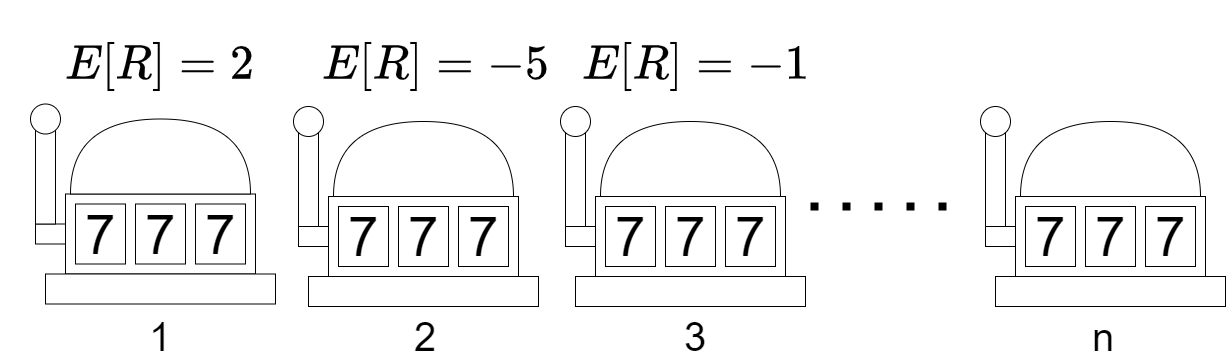
\includegraphics[width=1\textwidth]{losimoaparatai}
\caption{N lošimo aparatų, su skirtingais vidutiniais laimėjimais}
\label{losimoaparatai}
\end{figure}


Dažniausiai pateikiamas pavyzdys, kuris iliustruoja šio mokslo principą bei padeda geriau suprasti šiuos kintamuosius, yra lošimo aparatu, pavaizduotų \ref{losimoaparatai} paveikslėlyje, laimėjimų optimizavimas. Šiame uždavinyje iš n aparatų agentas bando surasti lošimo aparatą, kuris suteikia didžiausią įmanomą apdovanojimą. Kiekvienas aparatas duoda atsitiktinį laimėjimą iš  $\mathcal{N}(\mu=\mathcal{N}(0,2),\sigma=1)$ pasiskirstymo. Žaidimo sesija, dažniausiai vadiname epizodas, nėra ribojama, agentas gali atlikti begalybę $t$ žingsnių, lošimo aparatų pasirinkimų. Pasirinkimą galima traktuoti kaip veiksmą $a$ ir gautą laimėjimą kaip $r$. Agentas bando vienos žaidimo sesijos metu įgyti didžiausią sukauptą laimėjimą. Jis pritaiko viena iš populiariausiu skatinamojo mokslo metodu $\epsilon-godusis$. Šis metodas visados renkasi lošimo aparatą, kurio aproksimuotas tikėtinas laimėjimas, žymimas $Q(a)$, yra didžiausias, kaip tai išreikšta \ref {eqn:argmaxA} formulėje.

\begin{equation}
\label{eqn:argmaxA}
\begin{gathered}
A_t = argmax_aQ_t(a)
\end{gathered}
\end{equation}

Tačiau su maža $\epsilon$ tikimybe, agentas pasirenka atsitiktinį lošimo aparatą. Taigi kiekviename $t$ žingsnyje agentas renkasi lošimo aparatą, jį aktyvuoja ir gauną naują apdovanojimą, kuri talpina į to aparato apdovanojimų sąrašą. Šis procesas ypatingai svarbus, jis dominuoja visuose mokymosi modeliuose. Agentas stengiasi ne tik gauti didžiausia įmanomą tikėtiną laimėjimą, tačiau su $\epsilon$ tikimybe kartu tyrinėja aplinką, ieško optimalesnių lošimo aparatų, nei surastas dabartinis geriausias. Šis procesas vadinasi apdovanojimų-tyrinėjimo  kompromisu. Lošimo aparato tikėtinas laimėjimas tėra to aparato gautų laimėjimų vidurkis, kaip tai matosi \ref{eqn:Q(a)} formulėje.

\begin{equation}
\label{eqn:Q(a)}
\begin{gathered}
Q_t(a) = \frac{\sum_{i=1}^{t-1}R_i*\mathbb{1}_{A_i=a}} {\sum_{i=1}^{t-1}\mathbb{1}_{A_i=a}}
\end{gathered}
\end{equation}

Kitaip tariant $Q_t(a)$ yra apdovanojimų suma, kuomet pasirinkome $a$ veiksmą (arba lošimo aparatą), atlikus $t$ žingsnių, padalinti iš kiek kartų buvo $a$ veiksmas (arba lošimo aparatas) pasirinktas. Kuomet $t$ artėja link begalybės, vadovaujantis didžiųjų skaičių dėsniu, $Q(a)$ priartėja prie tikrosios reikšmės. Visi naujausi modeliai yra paremti panašiu imties traukimo metodu - simuliuojame skirtingus veiksmus ir stebime gautus rezultatus. Nors pavyzdys atrodo primityvus, tačiau visi naujausi modeliai sprendžia tą pačią užduoti - kokį pasirinkti veiksmą $a$, kuris suteiktų didžiausią apdovanojimą. 

Pagrindiniai skirtumai tarp metodų atsiranda dėl kompiuterio resursų optimizavimo. Viena iš problemų, su kuria iškarto susiduriame, yra duomenų kaupimas. Kiekvienam lošimo aparatui reikia kaupti jo gautus apdovanojimus. Didėjant problemai bei jos duomenų dimensijai, kompiuteriui kaupti duomenis tampa fiziškai nebeįmanoma, todėl yra sukurta daugybe esminių metodų šią problemą mažinti bei išvengti. Vienas iš metodų, kurio formą galima pastebėti TD formulėje, yra rekursyvus vidurkio apskaičiavimas, pateiktas \ref{eqn:Vidurkio} formulėje. Ši formule padeda išvengti apdovanojimų kaupimo, kaip tai matėme lošimo pavyzdyje.

\begin{equation}
\label{eqn:Vidurkio}
\begin{aligned}
Q_{n+1} &=\frac{1}{n} \sum_{i=1}^{n} R_{i} \\
&=\frac{1}{n}\left(R_{n}+\sum_{i=1}^{n-1} R_{i}\right) \\
&=\frac{1}{n}\left(R_{n}+(n-1) \frac{1}{n-1} \sum_{i=1}^{n-1} R_{i}\right) \\
&=\frac{1}{n}\left(R_{n}+(n-1) Q_{n}\right) \\
&=\frac{1}{n}\left(R_{n}+n Q_{n}-Q_{n}\right) \\
&=Q_{n}+\frac{1}{n}\left[R_{n}-Q_{n}\right]
\end{aligned}
\end{equation}

Lošimų pseudokodas, kuris palaipsniui apskaičiuoja skirtingų veiksmų imties vidurkius, pateiktas toliau:

\begin{algorithm}[H]
\label{LosimuAlgo}
\SetAlgorithmName{Algoritmas}{}
\SetAlgoLined

$Q(a) \leftarrow 0$\;
$N(a) \leftarrow 0$\;

 \For{$ \infty $}{
	$$ A \leftarrow \begin{cases}\arg \max _{a} Q(a) \text { su tikimybe } 1-\varepsilon \text { (lygiąsias reikšmes pasirenkame atsitiktinai) } \\
\text {atsitiktinis veiksmas } \text { su tikimybe} \varepsilon\end{cases}$$
	$R \leftarrow \text { LošimoAparatas }(A) $ \tcp*{Pasirenkame veiksma A ir gauname apdovanojimą R}
	$N(A) \leftarrow N(A)+1 $ \tcp*{Kiek kartų kiekvienas veiksmas buvo pasirinktas}
	$Q(A) \leftarrow Q(A)+\frac{1}{N(A)}[R-Q(A)]$\;
    }
\KwResult{ Gautos optimalios, tikrosios Q(a) reikšmės. Jas turint žinosime, kuris aparatas duoda didžiausią laimėjimą}
 \caption{Lošimo aparato pseudo algoritmas}
\end{algorithm}


Paskutinė \ref{eqn:Vidurkio} formulės išraiška yra ypatingai svarbi, nes ji yra ištaka tiek TD, tiek Q-mokymosi, tiek Bellmano formulėms, kurios yra skatinamojo mokslo pamatas. Apibendrinant \ref{eqn:Vidurkio} formulę ją galima šitaip išreikšti:

\begin{equation}
\text{Naujas vidurkis = Senas vidurkis }+ \frac{1}{n} (\text{Nauja reikšmė - Senas vidurkis})
\end{equation}

Jei tęstume formules apibendrinimą išryškėtu Bellmano funkcija, kuri yra viena svarbiausiu šiame moksle ir į kuria gilinsimės tolimesniuose skyriuose:

\begin{equation}
\label{TDLietuviskai}
\text{Naujas įvertis = Senas įvertis}+ \frac{1}{n} * (\textbf{Tikslas - Senas įvertis})
\end{equation}

Paryškinta dalis yra vadinama TD paklaida, ties kuria gilinsimes tolimesniuose skyriuose.

Kol kas nagrinėta problema pasižymi apdovanojimo skirstino stacionarumu, jis nekinta. Tačiau nagrinėjant sudėtingas problemas netik mūsų apdovanojimų pasiskirstymas kinta, tačiau mums įdomios tik paskutinės 10 -100 reikšmės. Taip pat aukštos dimensijos problemose mums neužtenka kompiuterio resursų išsaugoti $N(A)$ reikšmių, ką mes atliekame \ref{LosimuAlgo} pseudokode. Todėl įgyvendinamas dar vienas \ref{eqn:Vidurkio} formulės optimizavimas, aptariamas sekančiame skyriuje.

%
\subsubsection{Ne stacionarus apdovanojimo skirstinys}
%

Galima pastebėti daugybę problemų su \ref{eqn:Vidurkio} formule:

\begin{enumerate}
  \addtolength{\itemsep}{-0.5\baselineskip} 
  \item Toliau plėtojant duotą pavyzdį, galima įsivaizduoti situaciją, kurioje, kas tam tikrą laiko intervalą, kiekvieno aparato apdovanojimo funkcija pakinta ir įgyja nauja $\mathcal{N}(\mu=\mathcal{N}(0,2),\sigma=1)$ pasiskirstymą.
  \item Kuomet vieno lošimo aparato apdovanojimų $R$ imtis yra labai didelė, naujai gautos reikšmės turi labai mažai įtakos vidurkio pokyčiui dėl $\frac{1}{n}$ formulėje esančios išraiškos.
  \item Kiekviena $Q(a)$ reikšmė turi kaupti $N(A)$. Aukštosiose dimensijos neužtenka kompiuterio resursų išsaugoti šias reikšmes.
\end{enumerate}

Šios problemos sprendimas jau buvo pateiktas Adamo algoritmo įgyvendinime, mes toliau naudojame slenkančio vidurkio principus:

\begin{equation}
\label{judantisVidurkis}
\begin{aligned}
Q_{n+1} &=Q_{n}+\alpha\left[R_{n}-Q_{n}\right] \\
&=\alpha R_{n}+(1-\alpha) Q_{n} \\
&=\alpha R_{n}+(1-\alpha)\left[\alpha R_{n-1}+(1-\alpha) Q_{n-1}\right] \\
&=\alpha R_{n}+(1-\alpha) \alpha R_{n-1}+(1-\alpha)^{2} Q_{n-1} \\
&=\alpha R_{n}+(1-\alpha) \alpha R_{n-1}+(1-\alpha)^{2} \alpha R_{n-2}+\\
& \quad \ldots+(1-\alpha)^{n-1} \alpha R_{1}+(1-\alpha)^{n} Q_{1} \\
&=(1-\alpha)^{n} Q_{1}+\sum_{i=1}^{n} \alpha(1-\alpha)^{n-i} R_{i}
\end{aligned}
\end{equation}

Ši \ref{judantisVidurkis} formulė pakeičia $\frac{1}{n}$ į $\alpha \in [0,1]$. Dažniausia $\alpha$ reikšmė yra 0.9, su kuria apytiksliai apskaičiuojame paskutinių gautų 10-ties narių vidurkį.

\subsubsection{Markovo grandinės}

Dauguma mažos dimensijos skatinamojo mokslo problemų galima išreikšti Markovo grandinių pavidalu. Toks išreiškimas padeda geriau suvokti keturias pagrindines skatinamojo mokslo sąvokas:

\begin{enumerate}
  \addtolength{\itemsep}{-0.5\baselineskip} 
  \item \gls{s} - esama būsena. Pvz., automobilio momentinis greitis ar automobilio sensorių informacija.
  \item \gls{a} - pasirinktas veiksmas. Pvz., automobilio greičio pedalo paspaudimo stiprumas.
  \item \gls{r} - esamosios būsenos pasirinkto veiksmo apdovanojimas. Pvz., jei simuliuojamas automobilis pateko į avariją, jo apdovanojimas tampa neigiamas, gaunama bauda.
  \item $s\sp{\prime}$ - nauja būsena, kuri gaunama atlikus $a$ veiksmą.
\end{enumerate}

Nors dažniausiai būsenos būna daugiau nei vienos dimensijos, pavyzdžiui būsenos vektorius susidedantis iš 2 reikšmių - pozicijos bei greičio, lengviausiai jas yra suprasti atvaizduojant vienos dimensijos Markovo grandinių pavidalu, kaip tai matosi \ref{DulkiuSiurblys} paveikslėlyje.

\begin{figure}[h]
\centering
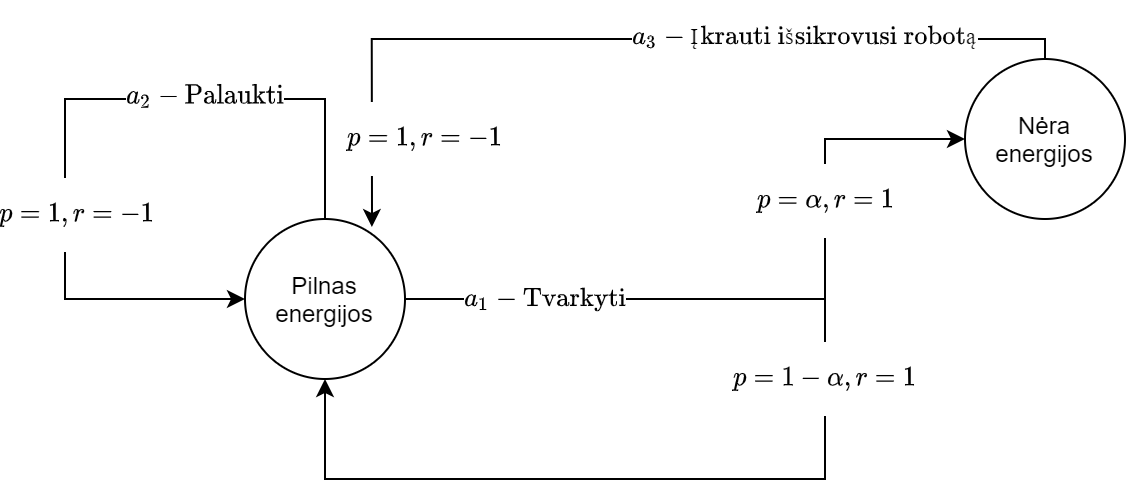
\includegraphics[width=1\textwidth]{DulkiuSiurblys}
\caption{Dulkio siurblio Markovo grandinė}
\label{DulkiuSiurblys}
\end{figure}

Pvz., jei dulkių siurblio robotas yra būsenoje $s = \text{(Pilnas energijos)}$, jis gali pasirinkti $a_1$ arba $a_2$ veiksmus. Pasirinkęs $a_1$ veiksmą, robotas su $\alpha$ tikimybe gali patekti į būsena $s\sp{\prime} = \text{(Nėra energijos)}$ ir su tikimybe $1-\alpha$ į būseną $s\sp{\prime} = \text{(Pilnas energijos)}$. Už abu šiuos veiksmus veiksmus robotas yra apdovanojamas $r=1$. Šis procesas galioja ir kitoms būsenoms. 

Priklausomai nuo esančios būsenos, mes visą laiką norime pasirinkti tokį veiksmą, kuris duoda didžiausią tikėtiną apdovanojimą:

\begin{equation}
r(s, a) \doteq \mathbb{E}\left[R_{t} \mid S_{t-1}=s, A_{t-1}=a\right]=\sum_{r \in \mathcal{R}} r \sum_{s^{\prime} \in \mathcal{S}} p\left(s^{\prime}, r \mid s, a\right)
\end{equation}

Veiksmų pasirinkimas vadovaujantis didžiausiu tikėtinu apdovanojimu bus nagrinėjamas sekančiame skyriuje.

Markovo grandinių išraiška taip pat yra svarbi ne tik dėl vizualinio aiškumo. Visos skatinamojo mokymo problemų formuluotės privalomai turi galėti išsireikšti Markovo grandinių pavidalu. Šis reikalavimas yra būtinas dėl vienos iš pagrindinių Markovo grandinės savybių - ateities įvykio tikimybė nepriklauso nuo prieš tai įvykusių įvykių:

\begin{equation}
P\left(X_{n+1}=x \mid X_{0}, X_{1}, X_{2}, \ldots, X_{n}\right)=P\left(X_{n+1}=x \mid X_{n}\right),
\end{equation}

kur $X$ yra prieš tai buvę įvykiai. Ši savybė leidžia apskaičiuoti tikėtiną apdovanojimą pasitelkiant tik turimą būseną, prieš tai buvusios būsenos neturi įtakos tikėtinam apdovanojimui.

Taigi \ref{DulkiuSiurblys} pavyzdys iliustruoja kaip skatinamajame moksle yra lengva apskaičiuoti naudingiausius veiksmus, kuomet turime sudaryta modelį. Tačiau retu atveju mes jį turime ir dažniausiai mums reikia imtis aplinkos tyrinėjimo veiksmų, kurie sudaro modelio aproksimacijas. Taip pat mes ne tik norime apskaičiuoti geriausią sekančio veiksmo apdovanojimą, tačiau geriausią apdovanojimą ilgalaikėje perspektyvoje. Dažnai gyvenime mes pasirenkame mėgautis maloniais dalykais, kuriais vėliau mes gailimės. Būtent šią problemą kitas skyrius ir nagrinės - ilgalaikis apdovanojimas, o ne trumpalaikis.

\subsubsection{Apdovanojimai bei tikslai}

Apdovanojimų hipotezė: kad visa tai, ką mes turime omenyje kalbėdami apie tikslus ir uždavinius, gali būti gerai suprantama kaip tikėtinos vertės didinimas, kai gaunama ilgalaikė skaliarinio signalo (vadinamo apdovanojimu) suma.

Šią sumą mes vieno epizodo metu stengiamės didinti. Epizodas - būsenų, veiksmų, apdovanojimų seka, kuri užsibaigę agentui pasiekus tikslą arba sustojimo sąlygą, kaip tai matome \ref{Episodas} paveikslėlyje. Agentas renkasi skirtingus veiksmus, įgauna naujas būsenas, kaupia epizodo apdovanojimą, kol galiausiai pasiekę tikslą, pavaizduotų pilku kvadratu.

\begin{figure}[h]
\centering
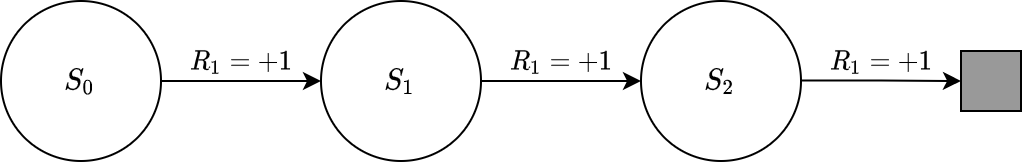
\includegraphics[width=0.8\textwidth]{Episodas}
\caption{Vienas agento epizodas}
\label{Episodas}
\end{figure}

Epizodo galutinis sukauptas apdovanojimas užrašomas tokiu pavidalu:

\begin{equation}
G_{t} \doteq R_{t+1}+R_{t+2}+R_{t+3}+\cdots+R_{T},
\end{equation}

kur $T$ yra paskutinis epizodo žingsnis. Tačiau jei agentas optimizuoja savo veiksmus aplinkoje, kurios pabaigą neįmanoma identifikuoti arba epizodas trunka nepaprastai daug žingsnių, mes naudojame apdovanojimų proporcionalius mažinimus:

\begin{equation}
G_{t} \doteq R_{t+1}+\gamma R_{t+2}+\gamma^{2} R_{t+3}+\cdots=\sum_{k=0}^{\infty} \gamma^{k} R_{t+k+1},
\end{equation}

kur $\gamma$ yra nuolaidos kintamasis, kurio dažniausia vertė yra 0.9. Ši vertė indikuoja, kad 11 žingsnio apdovanojimas bus proporcionalus $0.9^{11}$ savo vertės, kitaip tariant nuliui. Tačiau ši formulė kaip ir praeitos pasižymi panašiais trūkumais, kaip nuolatinis duomenų kaupimas. Tai galima išspręsti perrašius formulę į rekursinę formą:

\begin{equation}
\begin{aligned}
G_{t} & \doteq R_{t+1}+\gamma R_{t+2}+\gamma^{2} R_{t+3}+\gamma^{3} R_{t+4}+\cdots \\
&=R_{t+1}+\gamma\left(R_{t+2}+\gamma R_{t+3}+\gamma^{2} R_{t+4}+\cdots\right) \\
&=R_{t+1}+\gamma G_{t+1}
\end{aligned}
\end{equation}

Taip pat ši formulė padeda pasiekti balansą ties ilgalaikio apdovanojimo bei trumpalaikio apdovanojimo optimizavimo.

\label{apdovanojimoPatarimas}
Vienas iš svarbiausių praktinių patarimų, padedančių pasiekti didžiausią ilgalaikį apdovanojimą yra priskirti apdovanojimus už pasiektą tikslą, o ne skirti apdovanojimus už tai kaip mes norėtume, kad agentas pasiektų tikslą. Agentas mokymo procese turi pats atrasti optimaliausius veiksmus vedančius ties tiek tikslo pasiekimu, tiek didžiausiu epizodo apdovanojimu. Kitame skyriuje bus apibrėžiama, kaip būtent agentas optimizuoja savo elgesį, jo viena iš tikslo funkcijos konceptų, kurį gradientiniai metodai nuolatos optimizuoja.


\subsubsection{Vertės bei veiksmų taisyklių funkcijos}

Norint pasirinkti veiksmus, vedančius į būsenas, kurios suteikia didžiausią įmanoma apdovanojimą, mes turime kiekvienai būsenai priskirti tam tikrą matą. Todėl kiekviena būsena yra nusakoma pagal savo vertę. Ši vertė yra žymima \gls{vpi} ir nusako pasirinktos $s$ būsenos tikėtiną apdovanojimą: 

\begin{equation}
v_{\pi}(s) \doteq \mathbb{E}_{\pi}\left[G_{t} \mid S_{t}=s\right]=\mathbb{E}_{\pi}\left[\sum_{k=0}^{\infty} \gamma^{k} R_{t+k+1} \mid S_{t}=s\right], \text { visiems } s \in \mathcal{S}
\end{equation}

Žinant kiekvienos būsenos tikėtina apdovanojimą, mes visados galime rinktis tik tuos veiksmus, kurie veda į didžiausią apdovanojimą, didžiausią $v_\pi(s\sp{\prime})$. Šį pasirinkimą nusako veiksmų taisyklės. Tai yra tikimybių pasiskirstymas žymimas \gls{pi}, nurodantis būsenos $s$ visų veiksmų pasirinkimu pasiskirstymą. Kitaip tariant su kokia tikimybe mes pasirinktume veiksmą $a$ būnant būsenoje $s$, kaip tai matosi paveikslėlyje \ref{policy}.

\begin{figure}[h]
\centering
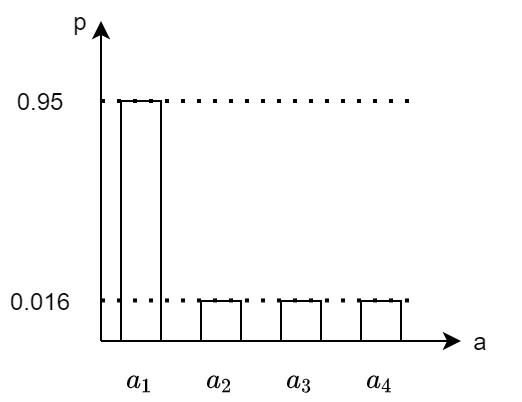
\includegraphics[width=0.6\textwidth]{policy}
\caption{Veiksmų taisyklių pasiskirstymas, kur $\epsilon= 5$}
\label{policy}
\end{figure}


Užrašymas $v_{\pi}(s)$ nurodo, kad ši būsenos vertė yra apskaičiuota naudojantis ${\pi}$ veiksmų taisyklėmis. Veiksmų taisyklės gali būti įvairios. Dažniausiai naudojame $\epsilon-godusis$ metodą, kaip tai matėme ties \ref{eqn:argmaxA} formule bei kurio pritaikymas Markovo grandinėms yra pateiktas \ref{eqn:greedyPolicy} formulėje. Šio metodu mes visą laiką priskiriame $1-\epsilon$ tikimybę veiksmui, kuris gražina didžiausią apdovanojimą apskaičiuojama naudojantis $v_{\pi}(s)$ formule. 

\begin{equation}
\label{eqn:greedyPolicy}
\begin{aligned}
\pi^{\prime}(s) & \doteq \underset{a}{\arg \max } q_{\pi}(s, a) \\
&=\underset{a}{\operatorname{argmax}} \mathbb{E}\left[R_{t+1}+\gamma v_{\pi}\left(S_{t+1}\right) \mid S_{t}=s, A_{t}=a\right] \\
&=\underset{a}{\operatorname{argmax}} \sum_{s^{\prime}, r} p\left(s^{\prime}, r \mid s, a\right)\left[r+\gamma v_{\pi}\left(s^{\prime}\right)\right]
\end{aligned}
\end{equation}


Turint kiekvienos būsenos taisyklių pasiskirstymą, galima suskaičiuoti kiekvienos būsenos tikėtiną reikšmę, kaip tai matosi \ref{eqn:tiketinaReiksme} formulėje.

\begin{equation}
\label{eqn:tiketinaReiksme}
\begin{aligned}
v_{\pi}(s) & \doteq \mathbb{E}_{\pi}\left[G_{t} \mid S_{t}=s\right] \\
&=\mathbb{E}_{\pi}\left[R_{t+1}+\gamma G_{t+1} \mid S_{t}=s\right] \\
&=\sum_{a} \pi(a \mid s) \sum_{s^{\prime}} \sum_{r} p\left(s^{\prime}, r \mid s, a\right)\left[r+\gamma \mathbb{E}_{\pi}\left[G_{t+1} \mid S_{t+1}=s^{\prime}\right]\right] \\
&=\sum_{a} \pi(a \mid s) \sum_{s^{\prime}, r} p\left(s^{\prime}, r \mid s, a\right)\left[r+\gamma v_{\pi}\left(s^{\prime}\right)\right], \quad \text { kiekvienam } s \in \mathcal{S},
\end{aligned}
\end{equation}

Šios formulės paskutinė lygybė yra dar geriau žinoma kaip Bellmano lygybė. Ji padeda rekursiškai apskaičiuoti $v_{\pi}(s)$ reikšmes bei išvengti apdovanojimų kaupimo kompiuterio atmintyje.

Tačiau praktikoje mes naudojame ne $v_{\pi}(s)$ - būsenos vertės matą, o \gls{qsa} - veiksmo vertės matą esant būsenoj $s$:

\begin{equation}
q_{\pi}(s, a) \doteq \mathbb{E}_{\pi}\left[G_{t} \mid S_{t}=s, A_{t}=a\right]=\mathbb{E}_{\pi}\left[\sum_{k=0}^{\infty} \gamma^{k} R_{t+k+1} \mid S_{t}=s, A_{t}=a\right]
\end{equation}

Galime pastebėti, kad $v_{\pi}(s)$ yra tos būsenos $s$ visų veiksmų $q_{\pi}(s, a)$ proporcinga $\pi(a|s)$ sudėtis bei taip pat išsireiškia Bellmano lygybe:

\begin{equation}
\begin{aligned}
& q_{\pi}(s, a)=E_{\pi}\left[G_{t} \mid S_{t}=s, A_{t}=a\right]=\\
&=\sum_{s^{\prime}} \sum_{r} p\left(s^{\prime}, r \mid s, a\right)\left[r+\gamma E_{\pi}\left[G_{t+1} \mid S_{t+1}=s^{\prime}\right]=\right.\\
=& \sum_{s^{\prime}} \sum_{r} p\left(s^{\prime}, r\mid s, a\right)\left[r \cdot \gamma \sum_{a^{\prime}} \pi\left(a^{\prime} \mid s^{\prime}\right) \cdot E_{\pi}\left[G_{t+1} \mid S_{t+1^{\prime}}=s^{\prime}, A_{t+1}=a^{\prime}\right]\right] \\
=& \sum_{s^{\prime}} \sum_{r} p\left(s^{\prime} r \mid s, a\right)\left[r+\gamma \sum_{a^{\prime}} \pi\left(a^{\prime} \mid s^{\prime}\right) \cdot q_{\pi}\left(s^{\prime}, a^{\prime}\right)\right],
\end{aligned}
\end{equation}

kur $v_{\pi}(s^{\prime}) = \gamma E_{\pi}\left[G_{t+1} \mid S_{t+1}=s^{\prime}\right]$.

Funkcijos $q_{\pi}(s, a)$ dėka mums nereikia apskaičiuoti $s$ būsenos visų veiksmų apdovanojimus norint gauti $v_{\pi}(s)$. Užtenka rinktis tik tuos veiksmus, kurie yra jau apskaičiuoti bei optimaliausi.

Taigi turint būsenų verčių bei veiksmų taisyklių apskaičiavimo formules galime pradėti iteracinį procesą, kurio tikslas yra optimizuoti šias reikšmes.

\subsubsection{Būsenų verčių bei veiksmų taisyklių iteravimas}

Optimizavimo metu, mes ieškome tokių \gls{BusenosVerte} bei optimalių taisyklių, kurios gražintų didžiausią epizodo apdovanojimą.
Yra daugybė būdų tai atlikti, kuriuos galima sugrupuoti į tris kategorijas:

\begin{enumerate}
  \addtolength{\itemsep}{-0.5\baselineskip} 
  \item dinaminio programavimo metodas, kuomet modelis žinomas, mes kiekvienos iteracijos metu perskaičiuojame visas $v_{\pi}(s)$ reikšmes ir atnaujiname \gls{VeiksmoTaisykles}. Šį procesą iteruojame, iki konvergacijos pasiekimo. Nenaudojamas metodas, nes labai retai tenkinama šio metodo privaloma sąlyga - modelio turėjimas. Modelį mes traktuojame kaip Markovo grandinių modelį, su visų veiksmų perėjimo tikimybėmis. Tačiau šio metodo dinaminėmis taisyklėmis remiasi vos ne visi naujausi metodai, todėl svarbu į šį metodą įsigilinti.
  \item Monte Carlo metodai - imties metodais apskaičiuojame $q_{\pi}(s, a)$ reikšmes. Šis metodas taikomas kuomet neturime modelio ir reikia jį aproksimuoti. 
  \item Neuroninių tinklų aproksimacijos - metodai, kurie aproksimuoja $q_{\pi}(s, a)$ reikšmes. Jei Monte Carlo metodai apskaičiuodavo kiekvienos būsenos tikslias reikšmes, funkcijų aproksimacijos metodais mes jas apskaičiuojame tik apytiksliai.
\end{enumerate}

Visos šios kategorijos pasižymi bendru optimizavimo principu:

\begin{enumerate}
  \addtolength{\itemsep}{-0.5\baselineskip} 
  \item įvertinimas - perskaičiuojame $v_{\pi}(s)$ reikšmes naudojantis atnaujintomis veiksmų taisyklėmis.
  \item tikslinimas - turint naujas $v_{\pi}(s)$ reikšmes, perskaičiuojame optimalias veiksmų taisykles $\pi(a|s)$.
\end{enumerate}

\begin{figure}[h]
\centering
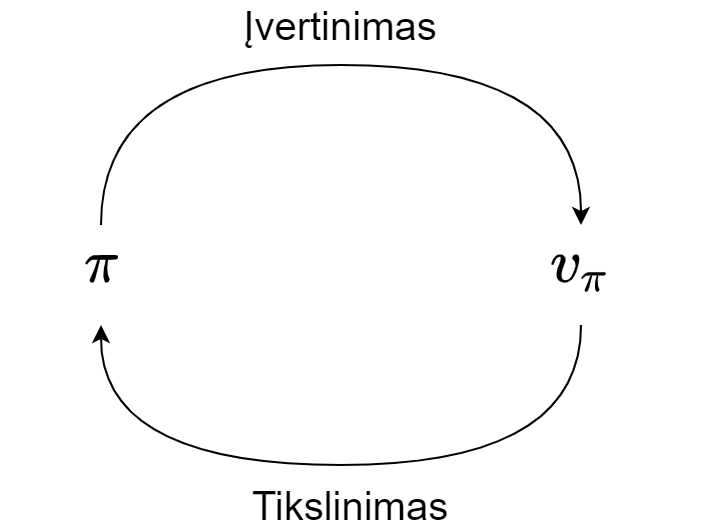
\includegraphics[width=0.5\textwidth]{policyIteration}
\caption{Viena optimizacijos iteracija }
\label{policyIteration}
\end{figure}

Šiuos žingsnius kartojame tol, kol pasiekiame $v_{\pi}(s)$ konvergaciją - naujos iteracijos nepakeičia $v_{\pi}(s)$ reikšmių. Tolimesniuose skyriuose trumpai apžvelgsiu šio proceso įgyvendinimą dinaminiuose bei Monte Carlo metoduose. Neuroninių tinklų aproksimacijos bus plėtojamos giliausiai, kadangi šiuo metu jie yra daugiau paplitę bei efektyviausi.

\subsubsection{Dinaminis programavimas}

Įvertinimo bei tikslinimo procesą, pateikta \ref{policyIteration} paveikslėlyje, paprasčiausiai iliustruoja dinaminio programavimo metodas pateiktas \ref{DynamicProgrammingExample} pavyzdyje. Šiame uždavinyje yra šešiolika langelių, ties kuriais agentas gali apsistoti. Du iš jų yra žali, žymi pozicijas, ties kuriomis agentas turi atsirasti. Agentas patekęs ant likusių baltų langelių turi nukakti į artimiausią žalią langelį. Agentas gali judėti tik keturiomis trajektorijomis, pateiktomis rodyklėmis. Kairėje paveikslėlio pusėje yra pateikti $v_{\pi}(s)$ įverčiai naudojantis \ref{eqn:tiketinaReiksme} formule, o dešinėje perskaičiuojame optimalias veiksmų taisykles naudojantis \ref{eqn:greedyPolicy} formule. Ypatingai svarbi optimizavimo seka:

\begin{enumerate}
  \addtolength{\itemsep}{-0.5\baselineskip} 
  \item Įvertinimas - Perskaičiuojame $v_{\pi}(s)$ reikšmes atnaujinamos naudojantis $t-1$ žingsnio taisyklėmis.
  \item Tikslinimas - Perskaičiavus $v_{\pi}(s)$ reikšmes, perskaičiuojame $t$ žingsnio optimalias veiksmų taisykles $\pi(a|s)$. Pavyzdyje naudojame godų veiksmo taisyklių įvertinima, kuris renkasi tik optimaliausius veiksmus.
\end{enumerate}

Vienas agento žingsnis, žymimas $t$, susideda iš šios įvertinimo bei tikslinimo sekos. Matome, kad užtenka vos trijų žingsnių veiksmų taisyklėms tapti optimaliomis. Tačiau $v_{\pi}(s)$ reikšmių konvergacija užtrunka ilgesni laiką. Įvykus konvergacijai, agentui atsiradus ant bet kurio iš galimų baltų langelių, jis, vadovaudamasis veiksmų taisyklėmis, visados optimaliai suras kelią į žalius langelius. Taip pat labai svarbu pastebėti seniau aptarta $v_{\pi}(s)$ išsiskaidymą į $q_{\pi}(s, a)$ narių sumą. Šis išsiskaidymas intuityviai matosi pateiktame \ref{DynamicProgrammingExample} paveikslėlio uždavinyje, kuomet kiekvieną rodyklę, galima traktuoti kaip $q_{\pi}(s, a)$ reikšmę.
$q_{\pi}(s, a)$ Išskaidymas yra svarbus neuroninių tinklų aproksimacijose, kaip tai bus aptarta tolimesniuose mokymosi modeliuose. Tačiau šis algoritmas yra tinkamas tik apskaičiuoti mažų dimensijų problemas bei iliustruoti intuityvius pavyzdžius. Augant tiek veiksmų, tiek būsenų erdvei šie skaičiavimai tampa neįmanomi. Ši problema plėtojama kitame skyriuje.


\begin{figure}[ht!]
\centering
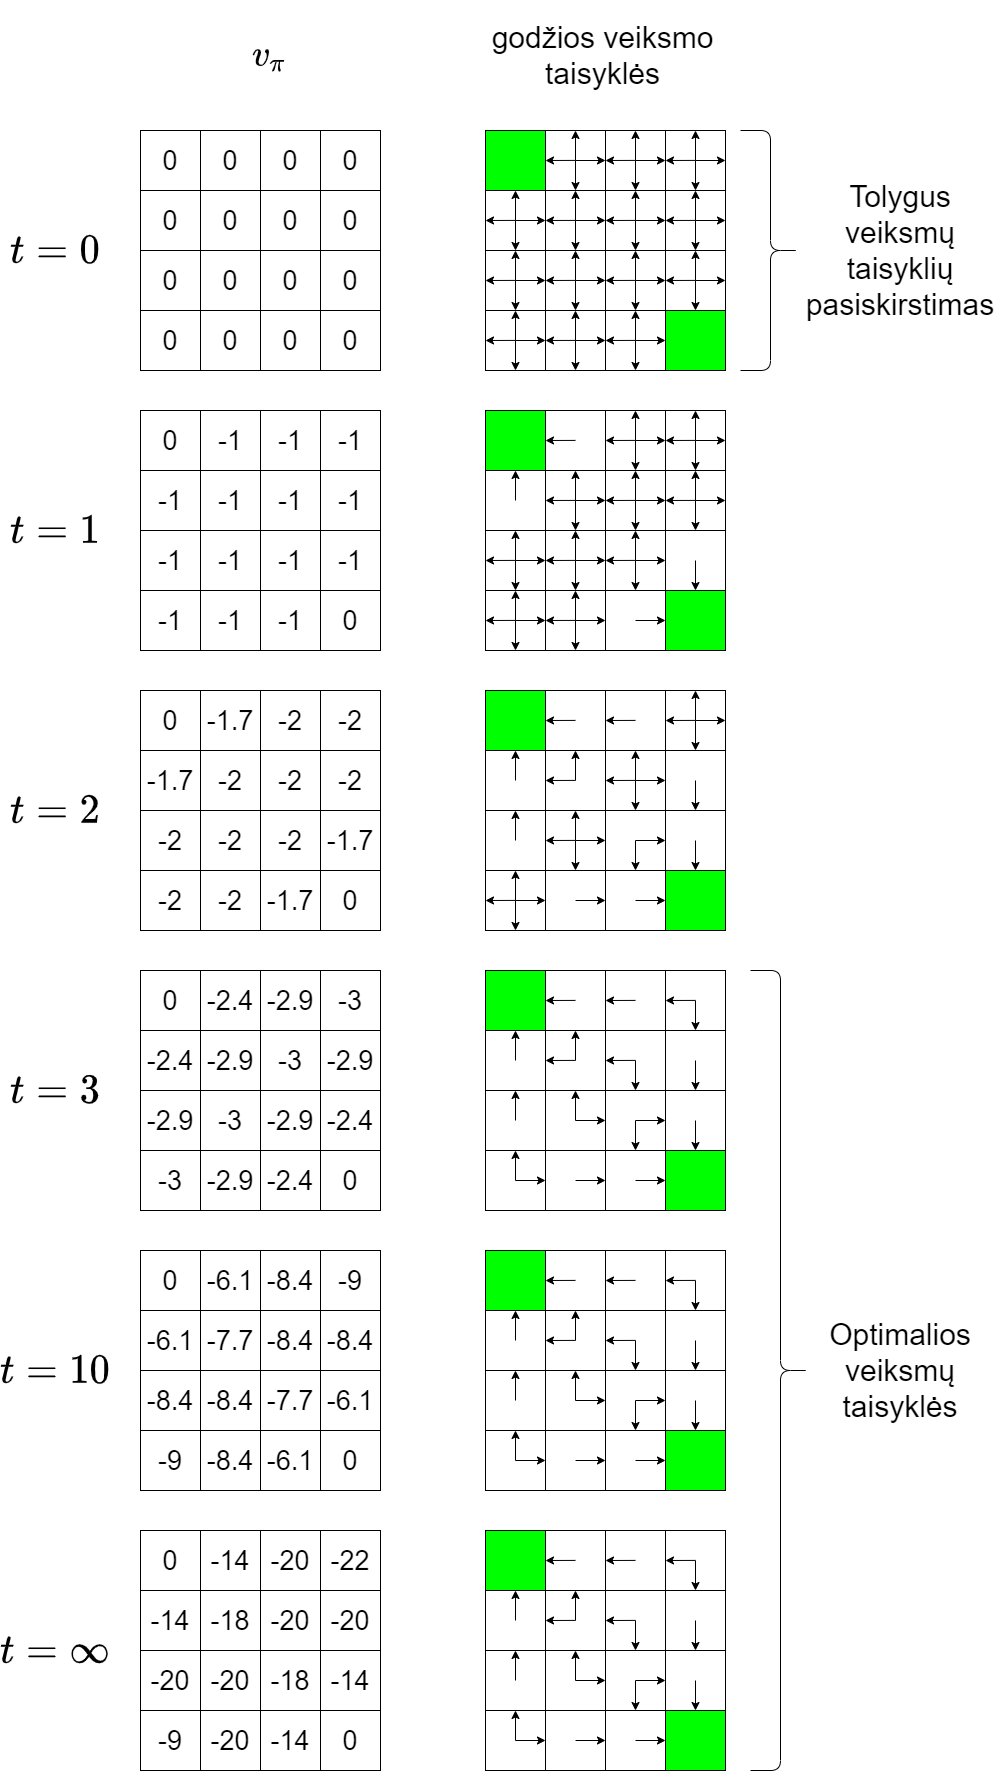
\includegraphics[width=0.8\textwidth]{DynamicProgrammingExample}
\caption{Dinaminio programavimo pavyzdys}
\label{DynamicProgrammingExample}
\end{figure}


\clearpage
\subsubsection{Monte Carlo metodai}

Nors specifinių Monte Carlo metodų šiame darbe nenagrinėsiu, tačiau pabrėšiu jų labai svarbų principą, kuriuo visi naujausi metodai remiasi. Monte Carlo metodais mes simuliuojame agento epizodus, gauname veiksmų trajektorijas (kaip tai matosi \ref{Episodas} paveikslėlyje) iš kurių susiskaičiuojame $q_{\pi}(s, a)$ reikšmes. Kiekvienos iteracijos metu kiekvienai būsenai $s$ bei jos specifiniui veiksmui $a$ mes išsaugome gautą apdovanojimą $G_t$. Iš šių išsaugotų reikšmių mes susiskaičiuojame vidurkį ir jį priskiriame $q_{\pi}(s, a)$ nariui. Tai atlikus mes perskaičiuojame veiksmų taisyklių reikšmes, kurios pasirenka naujus optimalius veiksmus. Po daugybes iteracijų, $q_{\pi}(s, a)$ konverguoja ties specifine, optimalia reikšme. Šio metodo veikimo principai pateikti \ref{alg:MC} pseudokode.

\begin{algorithm}[H]
 \label{alg:MC}
 \SetAlgorithmName{Algoritmas}{}
\SetAlgoLined
\DontPrintSemicolon
\textbf{Algoritmo parametrai:}\; 
$\varepsilon>0$\;
\textbf{Duomenų priskirimas:}\;

	$\pi \leftarrow$ atsitiktinė $\varepsilon$-greedy veiksmų taisyklių pasiskirstymas\;
	$Q(s, a) \in \mathbb{R}$ (atsitiktinis priskirimas), visiems $s \in \mathcal{S}, a \in \mathcal{A}(s)$\;
	Vertės $(s, a) \leftarrow$ tuščias sąrašas, visiems $s \in \mathcal{S}, a \in \mathcal{A}(s)$\;
	


 \For{$ \infty $}{
	Agentas sugeneruoja epizodą sekant $\pi: S_{0}, A_{0}, R_{1}, \ldots, S_{T-1}, A_{T-1}, R_{T}$\;
	$G \leftarrow 0$\;
	 \For{$t=T-1, T-2, \ldots, 0$}{
		$G \leftarrow \gamma G+R_{t+1}$\;
		\uIf{ Jei $S_{t}, A_{t}$ būsena yra pirmas apsilankymas  $S_{0}, A_{0}, S_{1}, A_{1} \ldots, S_{t-1}, A_{t-1}$ sekoje}{
    		Išsaugoti $G$ į Vertės$\left(S_{t}, A_{t}\right)$ sąraša\;
			$Q\left(S_{t}, A_{t}\right) \leftarrow$ vidurkis $\left(\right.$ Vertės$\left.\left(S_{t}, A_{t}\right)\right)$\;
			$A^{*} \leftarrow \arg \max _{a} Q\left(S_{t}, a\right)$\;
  			}
			\For{visi $a \in \mathcal{A}\left(S_{t}\right)$}{
			$
			\pi\left(a \mid S_{t}\right) \leftarrow \begin{cases}1-\varepsilon+\varepsilon /\left|\mathcal{A}\left(S_{t}\right)\right| & \text { if 			} a=A^{*} \\ \varepsilon /\left|\mathcal{A}\left(S_{t}\right)\right| & \text { if } a \neq A^{*}\end{cases}\;
			$
			}
		}
    }
\KwResult{ Gautos optimalios $Q(s, a)$ bei $\pi(a|s)$ reikšmės.}
\caption{Taisyklių bei verčių aproksimavimas Monte Carlo pirmo apsilankymo metodu}
\end{algorithm}

\ref{alg:MC} Algoritmo problema, kaip ir prieš tai buvusių metodų, yra kiekvienos būsenos ir jo veiksmo saugojimas bei ilgas konvergavimas. Augant būsenų bei veiksmų dimensijoms, konvergavimas tampa neįgyvendinama užduotimi. Veiksmams bei būsenoms užtenka būti trečioje dimensijoje ir jau nebeužtenka kompiuterio resursų apskaičiuoti optimalių reikšmių. Taip pat Monte Carlo metodai pasižymi duomenų kaupimo problema, kuomet neužtenka atminties juo saugoti. Duomenų kaupimą galima sumažinti pasitelkiant \ref{eqn:Vidurkio} bei \ref{judantisVidurkis} formulėmis, kaip tai atlieka pagrindinės šio mokslo formulės - TD ir Q-mokymasis.

\subsubsection{TD bei Q-mokymasis}

TD formulė sujungia Monte Carlo bei dinaminio programavimo pagrindines idėjas į vieną paprastą \ref{TD} formulę. 

\begin{equation}
\label{TD}
\begin{aligned}
V\left(S_{t}\right) &\leftarrow V\left(S_{t}\right)+\alpha\left[G_{t}-V\left(S_{t}\right)\right] = \\
& = V\left(S_{t}\right)+\alpha\left[R_{t+1}+\gamma V\left(S_{t+1}\right)-V\left(S_{t}\right)\right].
\end{aligned}
\end{equation}

Šios formulės ištakas galima pastebėti tiek \ref{eqn:Vidurkio} bei \ref{judantisVidurkis} formulėse. Šias dvi formules sujungus, galime perrašyti \ref{eqn:tiketinaReiksme} formulę, kuri pasitelkia Markovo grandinių modeliu, į \ref{TD} formulę, be Markovo grandinių modelio. TD paklaida yra paklaida tarp $R_{t+1}+\gamma V\left(S_{t+1}\right)$ bei $V\left(S_{t}\right)$ verčių, kaip tai matosi \ref{TD} formulėje. Kuomet $V\left(S_{t}\right)$ konverguoja, TD paklaida tampa nulinė. Pasiekus nulinę TD paklaidą galima laikyti, kad modelis yra tikslus. Vienas iš pagrindinių šio modelio skirtumu lyginant su \ref{alg:MC} algoritmu, yra greitesnė konvergacija. Šis metodas nelaukia epizodo galo, o atlieka $v_{\pi}(s)$ verčių atnaujinimą kiekvieno agento žingsnio metu. TD metodas yra pagrindas SARSA bei Q-mokymosi metodams, kurie atlieka atnaujinimus $q_{\pi}(s, a)$ vertėms. Šios dvi metodologijos skiriasi savo optimalumo atradimu, SARSA naudojasi šia TD atnaujinimo formule:

\begin{equation}
Q(S, A) \leftarrow Q(S, A)+\alpha\left[R+\gamma Q\left(S^{\prime}, A^{\prime}\right)-Q(S, A)\right].
\end{equation}

o Q-mokymasis šia:

\begin{equation}
\label{TD-Q}
Q(S, A) \leftarrow Q(S, A)+\alpha\left[R+\gamma \max _{a} Q\left(S^{\prime}, a\right)-Q(S, A)\right].
\end{equation}

Nors šios formulės yra vos ne identiškos, tačiau jos skiriasi skirtingomis optimaliomis veiksmų trajektorijomis. SARSA modelio atveju agentas stengiasi elgtis saugiai, dažniau vengia būsenų, kurių vertė yra neigiama. Šis modelis tinkamas tokiems eksperimentams, kuriuos yra brangu simuliuoti ir norime sumažinti agento kritines klaidas besimokant, vedančias ties agento fiziniu sugedimu, praradimu. Šio atvejo pavyzdys galėtų būti roboto navigacija ties šlaitu. Kiekvienos simuliacijos metu agentui besimokant jis gali nukristi nuo šlaito ir sugadinti savo įranga. Todėl norint šias brangias klaidas sumažinti mes apmokome robotą pasitelkiant SARSA metodu. Bet kadangi didžiąja laiko dalį mokymasis vyksta simuliuotose aplinkose, mūsų agento kritinių klaidų kaina nėra faktorius. Svarbiausias tikslas mums tampa optimalios verčių suradimas, kuo Q-mokymasis ir pasižymi. Q-mokymasis \cite{QLearning} yra vienas iš populiariausių bei seniausių egzistuojančių metodu. Tačiau jis išpopuliarėjo visai neseniai, kuomet 2014 metais Google Deepmind komanda sugebėjo \ref{TD-Q} funkcija aproksimuoti pasitelkiant konvoliucinius neuroninius tinklus. Šiomis aproksimacijomis Deepmind komanda apmokė agentus įveikti Atari žaidimus taip pademonstruojant skatinamojo mokymosi bei neuroninių tinklų aproksimacijų potencialą. Visi dabartiniai modeliai pasitelkia neuroninių tinklų aproksimacijomis. Aproksimacijos padėjo išspręsti viena didžiausių skatinamojo mokslo problemų - aukštų būsenų dimensijų neįmanoma konvergavimą. Dėl šios priežasties toliau bus aptariamas gilusis-Q - vienas iš pirmųjų, jau nebeefektyviu modeliu, sukėlusių skatinamojo mokslo atgimimą.

\subsubsection{Gilusis skatinamasis mokslas, gilusis-Q}
\label{GilusisQSkyrius}
Visi naujausi, dabartiniai skatinamojo mokslo modeliai yra aproksimuojami neuroniniais tinklais. Neuroniniai tinklai padeda generalizuoti nepaprastai didžiules būsenų erdves, kaip tai pademonstravo Google Deepmind giliojo-Q konvoliucinis neuroninis tinklas\cite{AtariGoogle}, kurio įvestis buvo kompiuterio ekrano individualūs pikseliai. 

Gilusis-Q metodas parametrizuoja $q_{\pi}(s, a)$ apdovanojimų vertę ir užrašoma $q_{\pi}(s, a, \theta)$ funkcijos pavidalu, kur $\pi$ yra veiksmų taisyklių tikimybių pasiskirstymas, kaip tai matėme \ref{policy} paveikslėlyje. Jo $\theta$ parametrai tampa neuroninio tinklo $\theta$ parametrai, kurie yra gradientiniais metodais optimizuojami, su tikslu pasiekti tikrąsias optimalias $q_{\pi}(s, a)$ reikšmes. Gilusis-Q neuroninio tinklo išvestis yra aproksimuota $q_{\pi}(s, a)$ reikšmė, kuri yra pateikta Q-mokymosi \ref{TD-Q} formulėje šiuo $\left[R+\gamma \max _{a} Q\left(S^{\prime}, a\right)\right]$ pavidalu. Kaip matome, mus domina tik pateiktos funkcijos tikslo dalis, kaip tai išreikšta \ref{TDLietuviskai} formulėje. Šis tikslas yra traktuojamas, kaip naujausia $q_{\pi}(s, a)$ reikšmė. Dažnai norint tai pabrėžti Q-mokymosi formulė yra pertvarkoma į \ref{QTikslas} formulėje pateiktą Bellmano pavidalą:

\begin{equation}
\label{QTikslas}
Q^{\text {naujas }}\left(s_{t}, a_{t}\right) \leftarrow(1-\alpha) \cdot \underbrace{Q\left(s_{t}, a_{t}\right)}_{\text{Sena reikšmė}}+\alpha \cdot\underbrace{(r_{t}+\gamma \cdot \max _{a} Q\left(s_{t+1}, a\right))}_{\text{Tikslas = nauja $q_{\pi}(s, a)$ reikšmė}}
\end{equation} 


Šis pavidalas yra nekas kitas, o daugybę kartu nagrinėta slenkančio vidurkio formulė, kur $\left[R+\gamma \max _{a} Q\left(S^{\prime}, a\right)\right]$ yra naujausia gauta $q_{\pi}(s, a)$ reikšmė.

Taigi neuroninis tinklas stengiasi aproksimuoti tikslą, kuris geriau žinomas kaip $G_t$ arba naujausias aproksimuotas $q_{\pi}(s, a)$ narys. Tuo tarpu neuroninio tinklo įvestis yra būsenos vektorius $s$. Kadangi naudojamas neuroninis tinklas, vektoriaus $s$ dydis nėra svarbus, konvergacija išlieka sparti. 

Optimizavimo procesas susideda iš šių trijų dalių:

\begin{enumerate}
  \addtolength{\itemsep}{-0.5\baselineskip} 
  \item sukuriama duomenų talpykla bei du neuroniniai tinklai - taikinys bei pagrindinis;
  \item pasirenkame veiksmą vadovaujantis godžiuoju $\epsilon$ veiksmų taisyklių metodu;
  \item svorių atnaujinimas naudojantis Bellmano taisykle, pateikta \ref{QTikslas}.
\end{enumerate}

\paragraph{Patirčių talpyklos bei dviejų neuroninių tinklų sukūrimas.}
\label{TalpyklosSkyrius}
Agentas tyrinėdamas aplinką, kaupia duomenis patirčių talpykloje, dar kitaip vadinama buferiu. Ši patirčių talpykla yra agento praeities patirtys, kurios padeda optimizuoti neuroninius tinklus. Joje kaupiamos $(s,a,r,s^\prime)$ duomenų eilutės, kurios vos ne identiškos SARSA modelio duomenims. Panašumas ties tuo nesibaigia, modelis taip pat kaupia duomenis tokiu pačiu principu kaip SARSA modelis, Monte Carlo būdu simuliuojant žingsnius. Esant būsenoje $s$ pagrindinis neuroninis tinklas aproksimuoja $s$ būsenos visų $a$ veiksmų $q_{\pi}(s, a)$ vertes, kaip tai matyti \ref{QNeuroniniaiTinklai} paveikslėlyje ir pasirenka judėti ta trajektorija, kurios $q_{\pi}(s, a)$ vertė yra didžiausia. 

\begin{figure}[h]
\centering
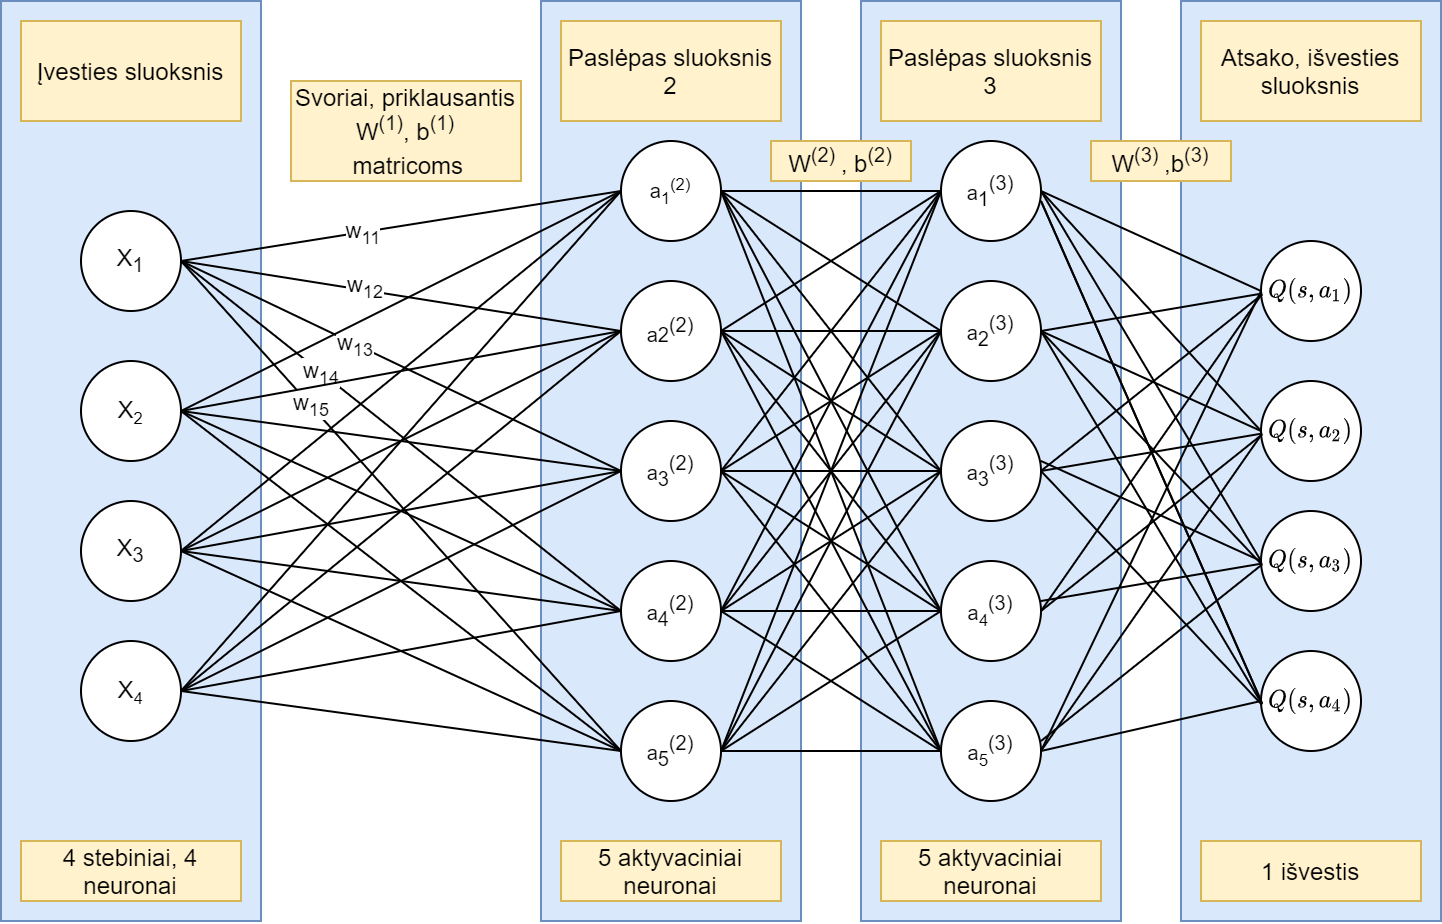
\includegraphics[width=1\textwidth]{Q Neuronu diagrama}
\caption{Giliojo Q neuroninio tinklo struktūra}
\label{QNeuroniniaiTinklai}
\end{figure}


Atlikus veiksmą, mes apskaičiuojame gautą apdovanojimą $r$ bei naują būseną $s^\prime$, kurioje atsiradome atlikus veiksmą $a$. Tokiu būdu turim vieną duomenų eilutę, kurią išsaugome į patirčių talpyklą. Sukaupus pakankamai daug duomenų galime juos pradėti naudoti neuroninio tinklo apmokymui. Apmokant mes pasitelkiame tik mažą dalį duomenų atsitiktinai ištrauktų iš talpyklos. Svarbu neuroninį tinklą apmokyti tik su duomenimis iš patirčių talpyklos, norint išvengti koreliacijos, tarp veiksmų, nutinkančių vienas po kito. Šią koreliacijos tendenciją lengva pastebėti intuityviai išanalizavus patirčių talpyklos veikimo principus.

\begin{enumerate}
  \addtolength{\itemsep}{-0.5\baselineskip} 
  \item Atsitiktinės duomenų eilutės $(s,a,r,s^\prime)$ paimamos iš patirčių talpyklos. Dėl atsitiktinio ėmimo, didžioji dalis patirčių - duomenų eilučių, yra iš skirtingų trajektorijų, epizodų.
  \item Su paimtais duomenimis apmokome modelį. Šio proceso metu, dėl atsitiktinio ėmimo, skirtingos būsenos įgyją naujas $q_{\pi}(s, a)$ aproksimacijas. 
\end{enumerate}

Tuo tarpu be patirčių talpyklos, mes apmokytume neuroninį tinklą kiekvieno žingsnio metu. Tačiau kadangi nauji agento žingsniai priklauso nuo senesnių, mūsų duomenis taptų priklausomi. Tai pažeidžia stochastinio gradientinio nuolydžio vieną iš pagrindinių reikalavimų - imties stebiniai turi būti nepriklausomi. Tai nutikus modelis pradėtų dažniau rinktis pasikartojančias trajektorijas, diverguotų į ne optimalias trajektorijas. Patirties talpykla taip pat turi dar viena papildoma svarbų bruožą - pakartotinas apmokymas su tais pačiais duomenimis. Kadangi duomenis yra išsaugojami talpykloje, mes turime ne mažą tikimybę apmokyti neuroninį tinklą su tuo pačiu dėmeniu ne vieną kartą. Šis bruožas naudingas apmokyti neuroninį tinklą su retai pasitaikančiomis reikšmėmis. Patirčių talpykla dažniausiai turi fiksuotą dydį. Talpykla yra naudojama visuose algoritmuose, kurie naudoja neuroninių tinklų aproksimacijas. 

Patirčių talpykla padeda apmokyti pagrindinį neuroninį tinklą, kurio tikslo funkcija yra pateikta žemiau:

\begin{equation}
L(\theta)=\left[\left(\left(r+\gamma \max _{a t+1} Q\left(s_{t+1}, a_{t+1} ; \theta^{\text {taikinys }}\right)\right)-Q\left(s, a ; \theta^{\text {pagrindinis }}\right)\right)^{2}\right].
\end{equation}

Ši funkcija panaši į mažiausių kvadratų optimizavimo tikslo funkciją. Šioje funkcijoje neuroniniai tinklai stengiasi sumažinti paklaidą tarp tikrosios $q_{\pi}(s, a)$ vertės bei neuroninio tinklo pateiktos aproksimacijos. Pateikti $\theta$ parametrai atkeliauja iš taikinio bei pagrindinio neuroninio tinklo. Abu neuroniniai tinklai aproksimuoja $q_{\pi}(s, a)$. Tačiau taikinio neuroninio tinklo parametrai nėra apmokami, jie kas tam tikra agento žingsnių kieki yra periodiškai paimami iš pagrindinio neuroninio tinklo. Tuo tarpu pagrindinio neuroninio tinklo parametrai yra atnaujinami kas kiekviena žingsnį. Ši metodologija buvo pirma karta pritaikyta Google Deepmind komandos, kuriant Atari agentus \cite{GoogleDeepQLearning}. Jos tikslas yra sumažinti mokymosi divergacijas bei nestabilias $q_{\pi}(s, a)$ verčių svyravimus. Šios nepalankios savybės atsiranda iš neuroninių tinklų generalizacijos. Atnaujinus $q_{\pi}(s, a)$ reikšmes ir pakeitus $\theta$ parametrus, kartu pasikeičia kaimyninės $q_{\pi}(s^\prime, a)$ reikšmės, kitaip tariant mūsų taikinio reikšmės, jei naudotume viena neuroninį tinklą. Nuolat kintančios taikinio reikšmės veda prie nestabilaus konvergavimo, mūsų aproksimuojamos $q_{\pi}(s, a)$ reikšmės artėja link norimų $q_{\pi}(s, a)$ reikšmių, kurios dėl kiekvieno atnaujinimo kinta. Todėl yra sukuriamas antras neuroninis tinklas su fiksuotais parametrais, kurie stabilizuoja mokymosi procesą.

\paragraph{Veiksmų pasirinkimas.}

Gilusis Q naudoja godųjį-$\epsilon$ metodą veiksmų pasirinkimui, kur su $1-\epsilon$ tikimybe pasirinksime veiksmą vedanti į didžiausią $q_{\pi}(s, a)$. Šias $q_{\pi}(s, a)$ vertes apskaičiuoja neuroninis tinklas, kaip tai pateikta \ref{QNeuroniniaiTinklai} paveikslėlyje. Tačiau su $\epsilon$ tikimybe mes pasirinksime neoptimalią vertę. Tai padeda aplankyti naujas trajektorijas, tikintis surasti optimalesnius veiksmus.

\paragraph{Svorių atnaujinimas.}

Atlikus veiksmo pasirinkimą bei išsaugojus duomenis susijusius su šiuo veiksmu mes įgyvendiname viena agento žingsnį. Po kiekvieno žingsnio mes apmokome agentą tiksliau generalizuoti $q_{\pi}(s, a)$ reikšmes. Mokymo procese pasitelkiame patirčių talpyklą, kaip tai jau buvo aptarta \ref{TalpyklosSkyrius} skyriuje. Mokymosi procesas gali trukti porą dienų, priklausomai nuo nagrinėjamos aplinkos sunkumo.

Nors Q-mokymasi procesas pademonstravo skatinamojo mokslo potencialą, šis metodas nebetaikomas. Tačiau svarbios pademonstruotos idėjos kaip  $q_{\pi}(s, a)$ verčių aproksimavimas neuroniniais tinklais, patirčių talpykla, dviejų neuroninių tinklų stabilizavimas yra pamatas aktoriaus-kritiko šablonui, kuriuo vadovaujasi visi moderniausi modeliai. Norint suprasti aktoriaus-kritiko šabloną, aptariama sekančiame skyriuje, pradžioje reik įsigilinti į vieną svarbiausių skatinamojo mokslo teoremų - veiksmo taisyklių gradientas.


\subsubsection{Veiksmo taisyklių gradientas bei aktorius-kritikas}

Veiksmo taisyklių parametrizavimas bei šios parametrizuotos funkcijos gradientas yra viena iš svarbiausių šio mokslo atradimų. Ilgą laiką buvo manoma, kad veiksmo taisyklių gradientas neegzistuoja, todėl buvo taikomi Giliojo-Q mokymosi algoritmai, kurie optimizuoja $q_{\pi}(s, a)$ vertes ir neliečia veiksmo taisyklių optimizavimo. Tačiau kaip matome \ref{policyIteration} paveikslėlyje, optimizavimo procesas įtraukia nuolatinį verčių bei veiksmo taisyklių iteravimą. Atradus veiksmo taisyklių gradientą, pagaliau tapo įmanoma įgyvendinti \ref{policyIteration} ciklą ir tai pasiekus gimė daugybė galingu modelių kaip PPO, DDPG, TD3, SAC. 

Veiksmo taisyklių tikslas yra skatinti tuos veiksmus, kurie vedė ties veiksmų trajektorijomis suteikiančiomis aukštus apdovanojimus ir slopinti veiksmus, kurių apdovanojimų trajektorijos yra mažos. Formaliai tai mes užrašome šiuo pavidalu, nurodančiu tikėtiną veiksmų taisyklių apdovanojimą:

\begin{equation}
J\left(\pi_{\theta}\right)=\underset{\tau \sim \pi_{\theta}}{\mathrm{E}}[R(\tau)],
\end{equation}

kur $R(\tau)$ yra gautų epizodo, trukusio $T$ žingsnių, apdovanojimų suma:

\begin{equation}
R(\tau) = \sum_{t=0}^{T} R_{t}.
\end{equation}

$J\left(\pi_{\theta}\right)$ yra tikėtinas apdovanojimas vadovaujantis $\pi$ veiksmo taisyklėmis, aproksimuotomis neuroninio tinklo $\theta$ parametrais.

Tikėtiną veiksmo taisyklių apdovanojimą mes išreiškiame per tikimybę įgyti šiuos apdovanojimus:

\begin{equation}
\label{Ptikimybes}
P(\tau \mid \theta)=\rho_{0}\left(s_{0}\right) \prod_{t=0}^{T} P\left(s_{t+1} \mid s_{t}, a_{t}\right) \pi_{\theta}\left(a_{t} \mid s_{t}\right)
\end{equation}

$P(\tau \mid \theta)$ yra trajektorijos tikimybė, kur $\rho_{0}\left(s_{0}\right)$ yra tikimybė, kad pradėsime $s_0$ būsenoje. Šią tikimybę sudauginus su apdovanojimų kiekiu, gauname galutinę $J(\pi)$ išraišką:

\begin{equation}
J(\pi)=\int_{\tau} P(\tau \mid \pi) R(\tau)=\underset{\tau \sim \pi}{\mathrm{E}}[R(\tau)]
\end{equation}

Mūsų tikslas yra optimizuoti veiksmų taisyklių $J(\pi)$ parametrus taip, kad jie gražintu kuo didesnį epizodų apdovanojimus:

\begin{equation}
\theta_{k+1}=\theta_{k}+\left.\alpha \nabla_{\theta} J\left(\pi_{\theta}\right)\right|_{\theta_{k}}
\end{equation}

Deja mes negalime optimizuoti $J(\pi)$ tiesiogiai, kadangi neturint modelio, mes negalime gauti \ref{Ptikimybes} formulės reikšmes, reikalingas apskaičiuoti gradientą. Todėl imamės analitinių išraiškų, padedančių pakeisti gradiento formulę į naują formulę, kurios rezultatas nors ir nesutampa su $J(\pi)$ bet sutampa jo gradientas. Šios formulės išvedimui buvo pasitelkti šie faktai:

\begin{enumerate}
  \addtolength{\itemsep}{-0.5\baselineskip} 
  \item Log išvestinė:
\begin{equation}
\nabla_{\theta} P(\tau \mid \theta)=P(\tau \mid \theta) \nabla_{\theta} \log P(\tau \mid \theta).
\end{equation}
  \item Log trajektorijos tikimybė:
\begin{equation}
\log P(\tau \mid \theta)=\log \rho_{0}\left(s_{0}\right)+\sum_{t=0}^{T}\left(\log P\left(s_{t+1} \mid s_{t}, a_{t}\right)+\log \pi_{\theta}\left(a_{t} \mid s_{t}\right)\right).
\end{equation}
  \item Apskaičiuojant gradientinį nuolydį, funkcijos, kurios nepriklauso nuo $\theta$, pranyksta. Kitaip tariant $\rho_{0}\left(s_{0}\right), P\left(s_{t+1} \mid s_{t}, a_{t}\right)$, ir $R(\tau)$ yra lygus nuliui.
 \item Šios pranykusios funkcijos supaprastina log trajektorijos tikimybe:
\begin{equation}
\begin{aligned}
\nabla_{\theta} \log P(\tau \mid \theta) &=\nabla_{\theta} \log _{0}\left(s_{0}\right)+\sum_{t=0}^{T}\left(\nabla_{\theta} \log P\left(s_{t+1} \mid s_{t}, a_{t}\right)+\nabla_{\theta} \log \pi_{\theta}\left(a_{t} \mid s_{t}\right)\right) \\
&=\sum_{t=0}^{T} \nabla_{\theta} \log \pi_{\theta}\left(a_{t} \mid s_{t}\right).
\end{aligned}
\end{equation}
\end{enumerate}

Pasitelkus šiuos išvedimus galime išsivesti veiksmo taisyklių gradientą:

\begin{equation}
\begin{array}{rlr}
\label{megaVeiksmuGradientas}
\nabla_{\theta} J\left(\pi_{\theta}\right) & =\nabla_{\theta_{\tau \sim \pi_{\theta}}} \underset{\tau \sim \pi_{\theta}}{\mathrm{E}}[R(\tau)]  \\
& =\nabla_{\theta} \int_{\tau} P(\tau \mid \theta) R(\tau)  \\
& =\int_{\tau} \nabla_{\theta} P(\tau \mid \theta) R(\tau)  \quad \quad \quad \quad \quad \quad \text { Log išvestinės faktas } \\
& =\int_{\tau} P(\tau \mid \theta) \nabla_{\theta} \log P(\tau \mid \theta) R(\tau)  \\
& =\underset{\tau \sim \pi_{\theta}}{\mathrm{E}}\left[\nabla_{\theta} \log P(\tau \mid \theta) R(\tau)\right]  \\
\therefore \nabla_{\theta} J\left(\pi_{\theta}\right) & =\underset{\tau \sim \pi_{\theta}}{\mathrm{E}}\left[\sum_{t=0}^{T} \nabla_{\theta} \log \pi_{\theta}\left(a_{t} \mid s_{t}\right) R(\tau)\right] \quad \text { 4 fakto pritaikymas }
\end{array}
\end{equation}

Turint šią formą mes stochastiniu būdu galime pradėti aproksimuoti gradientinį pakilimą. Šio proceso metu mes generuojame naujas imtis bei apskaičiuojame imties vidurkį:

\begin{equation}
\label{gGradientas}
\hat{g}=\frac{1}{|\mathcal{D}|} \sum_{\tau \in \mathcal{D}} \sum_{t=0}^{T} \nabla_{\theta} \log \pi_{\theta}\left(a_{t} \mid s_{t}\right) R(\tau),
\end{equation}

kur $\hat{g}$ yra veiksmo taisyklių gradiento vektorius, o $\mathcal{D}$ yra trajektorijų (imčių) kiekis. Tokiu būdu mes galime labai tiksliai aproksimuoti mūsų veiksmo taisyklių parametrus, vedančius ties didžiausiais apdovanojimais. 

Pats metodas savaime nėra efektyvus tačiau sukombinavus su Giliuoju-Q mokymusi mes grįžtame į pagrindinį \ref{policyIteration} metodą, kuris buvo taikomas be aproksimacijų. Šį procesą įgyvendina aktoriaus kritiko metodas. Jo pavadinimas kilo iš intuityvios idėjos, kuria galime pastebėti \ref{gGradientas} formulėje. Jei $R(\tau)$ yra teigiamas, pateiktas veiksmas paskatinamas, jei $R(\tau)$ neigiamas, pateiktas veiksmas slopinamas. $R(\tau)$ atlieka kritiko rolę, skatina arba slopina veiksmų taisyklių neuroninio tinklo, vadinamo aktoriumi, pateiktas reikšmes. Tačiau aktoriaus-kritiko metoduose mes vietoj tiesioginės $R(\tau)$ reikšmės, pasitelkiame giliojo-Q neuroninį tinklą kurio $q_{\pi}(s, a)$ reikšmės aproksimuoja $R(\tau)$. Taigi gilusis-Q pateikia $q_{\pi}(s, a)$ vertes bei jas optimizuoja, kaip tai jau matėme \ref{GilusisQSkyrius} skyriuje. Taip pat naudojantis $q_{\pi}(s, a)$ reikšmėmis mes kartu atnaujiname veiksmo taisyklių neuroninį tinklą naudojantis \ref{gGradientas} formule. Šis metodas bei jo pseudokodas bus toliau plėtojamas tolimesniuose modeliuose, kurie remiasi jo struktūra.

\subsubsection{DPG bei DDPG}

DPG\cite{DPG} metodas yra paremtas aktoriaus-kritiko metodu. Jis sujungia Gilusis-Q metodą su veiksmo taisyklių gradientu. Tačiau šiuo atveju veiksmo taisyklių tikslo formulė įgauna skirtingą pavidalą:

\begin{equation}
J(\theta)=\int_{\mathcal{S}} \rho^{\mu}(s) Q\left(s, \mu_{\theta}(s)\right) d s,
\label{netoksKeistasGradientas}
\end{equation}

kur $\mu_{\theta}(s)$ yra deterministinės funkcijos $\pi_\theta(a|s)$ atitikmuo. Kitaip tariant veiksmai parenkami ne iš veiksmų tikimybių pasiskirstymo, o optimaliausias veiksmas yra iškarto funkcijos aproksimuojamas - $a = \mu(s)$. Tuo tarpu $\rho^{\mu}(s)$ žymi tikimybę, kad pradėsime $s$ būsenoje, o $Q\left(s, \mu_{\theta}(s)\right)$ yra neparametrizuoto $q_{\pi}(s, a)$ atitikmuo. Veiksmų aproksimacijos padeda praplėsti veiksmų dimensiją iš keleto pasirinkimų, kaip tai matėme \ref{DynamicProgrammingExample} pavyzdyje, turint tik keturis galimus veiksmus, į begale. Vienas iš praktinių šio metodo bruožų yra jo gradiento apskaičiavimas:

\begin{equation}
\begin{aligned}
\nabla_{\theta} J(\theta) &=\left.\int_{\mathcal{S}} \rho^{\mu}(s) \nabla_{a} Q^{\mu}(s, a) \nabla_{\theta} \mu_{\theta}(s)\right|_{a=\mu_{\theta}(s)} d s \\
&=\mathbb{E}_{s \sim \rho^{\mu}}\left[\left.\nabla_{a} Q^{\mu}(s, a) \nabla_{\theta} \mu_{\theta}(s)\right|_{a=\mu_{\theta}(s)}\right]
\label{keistasGradientas}
\end{aligned}
\end{equation}

Telieka simuliuoti agento žingsnius ir apskaičiuoti veiksmo taisyklių gradientą, kaip tai matėme \ref{gGradientas} formulėje. Praktikoje gradiento apskaičiavimas yra keblesnis, nei \ref{megaVeiksmuGradientas} metodo, kadangi reikia apskaičiuoti dviejų neuroninių tinklų gradientus bei juos sudauginti. Šis procesas bus giliau aptariamas praktikoje. 

Šio modelio didžiausias trūkumas yra neegzistuojantis agento aplinkos tyrinėjimas. Modelis visados renkasi optimalias veiksmų taisykles, netyrinėja aplinkos. DDPG\cite{DDPG} modelis pagerina DPG modelį pridėdamas triukšmą prie veiksmų taisyklių pateiktų reikšmių:

\begin{equation}
\mu^{\prime}(s)=\mu_{\theta}(s)+\mathcal{N},
\end{equation}

kur $\mathcal{N}$ yra normalusis pasiskirstymas. Jo parametrai yra pasirenkami priklausomai nuo nagrinėjamos problemos. Taigi pridėjus prie aproksimuotos veiksmo reikšmės $\mu_{\theta}(s) \in \mathcal{R}$ mažą triukšmą, mes skatiname modelį rinktis įvaresnius veiksmus, leidžiančius surasti optimalesnes veiksmų trajektorijas.

\subsubsection{TD3}

TD3\cite{TD3} modelis yra vos ne identiškas DDPG modeliui tačiau turi pora skirtumu:

\begin{enumerate}
  \addtolength{\itemsep}{-0.5\baselineskip} 
  \item Du gilieji-Q neuroniniai tinklai. Kadangi gilusis-Q neuroninis tinklas dažnai pervertina reikšmes, mes apmokymui naudojame du giliuosius-Q neuroninius tinklus ir apmokome su mažesne gauta reikšme.
  \item Vėluojantis veiksmo taisyklių neuroninio parametrų atnaujinimas. Jei DPG atnaujindavo neuroninį tinklą kas kiekvieną agento žingsnį TD3 autorius rekomenduoja atnaujinimą atlikti kas du žingsnius. 
  \item Reguliarizacija, pateikta \ref{TD3Reg} formulėje. Ji padeda išvengti persimokymo, kuomet veiksmų taisyklės per greit prisitaiko prie aukštų gilaus-Q reikšmių. Pagrindinė idėja yra pridėti maža triukšmą prie veiksmo taisyklių neuroninio tinklo pateiktos reikšmės. Tokiu būdu neuroninis tinklas bus apmokytas geriau aproksimuoti kaimynines veiksmų reikšmes.
\end{enumerate}

\begin{equation}
\label{TD3Reg}
a^{\prime}\left(s^{\prime}\right)=\operatorname{clip}\left(\mu_{\theta_{\text {taikinio }}}\left(s^{\prime}\right)+\operatorname{clip}(\epsilon,-c, c), a_{\text {min }}, a_{max}\right), \quad \epsilon \sim \mathcal{N}(0, \sigma).
\end{equation}

TD3 struktūra susideda iš šešių neuroninių tinklų, kaip tai matosi \ref{TD3Struktura} paveikslėlyje. Jie reikalingi tiktais apmokymo metu. Apmokius neuroninį tinklą užtenka vieno veiksmų taisyklių neuroninio tinklo, kuris pateiktų optimalius veiksmus agentui.

\newpage
\begin{figure}[h!]
\centering
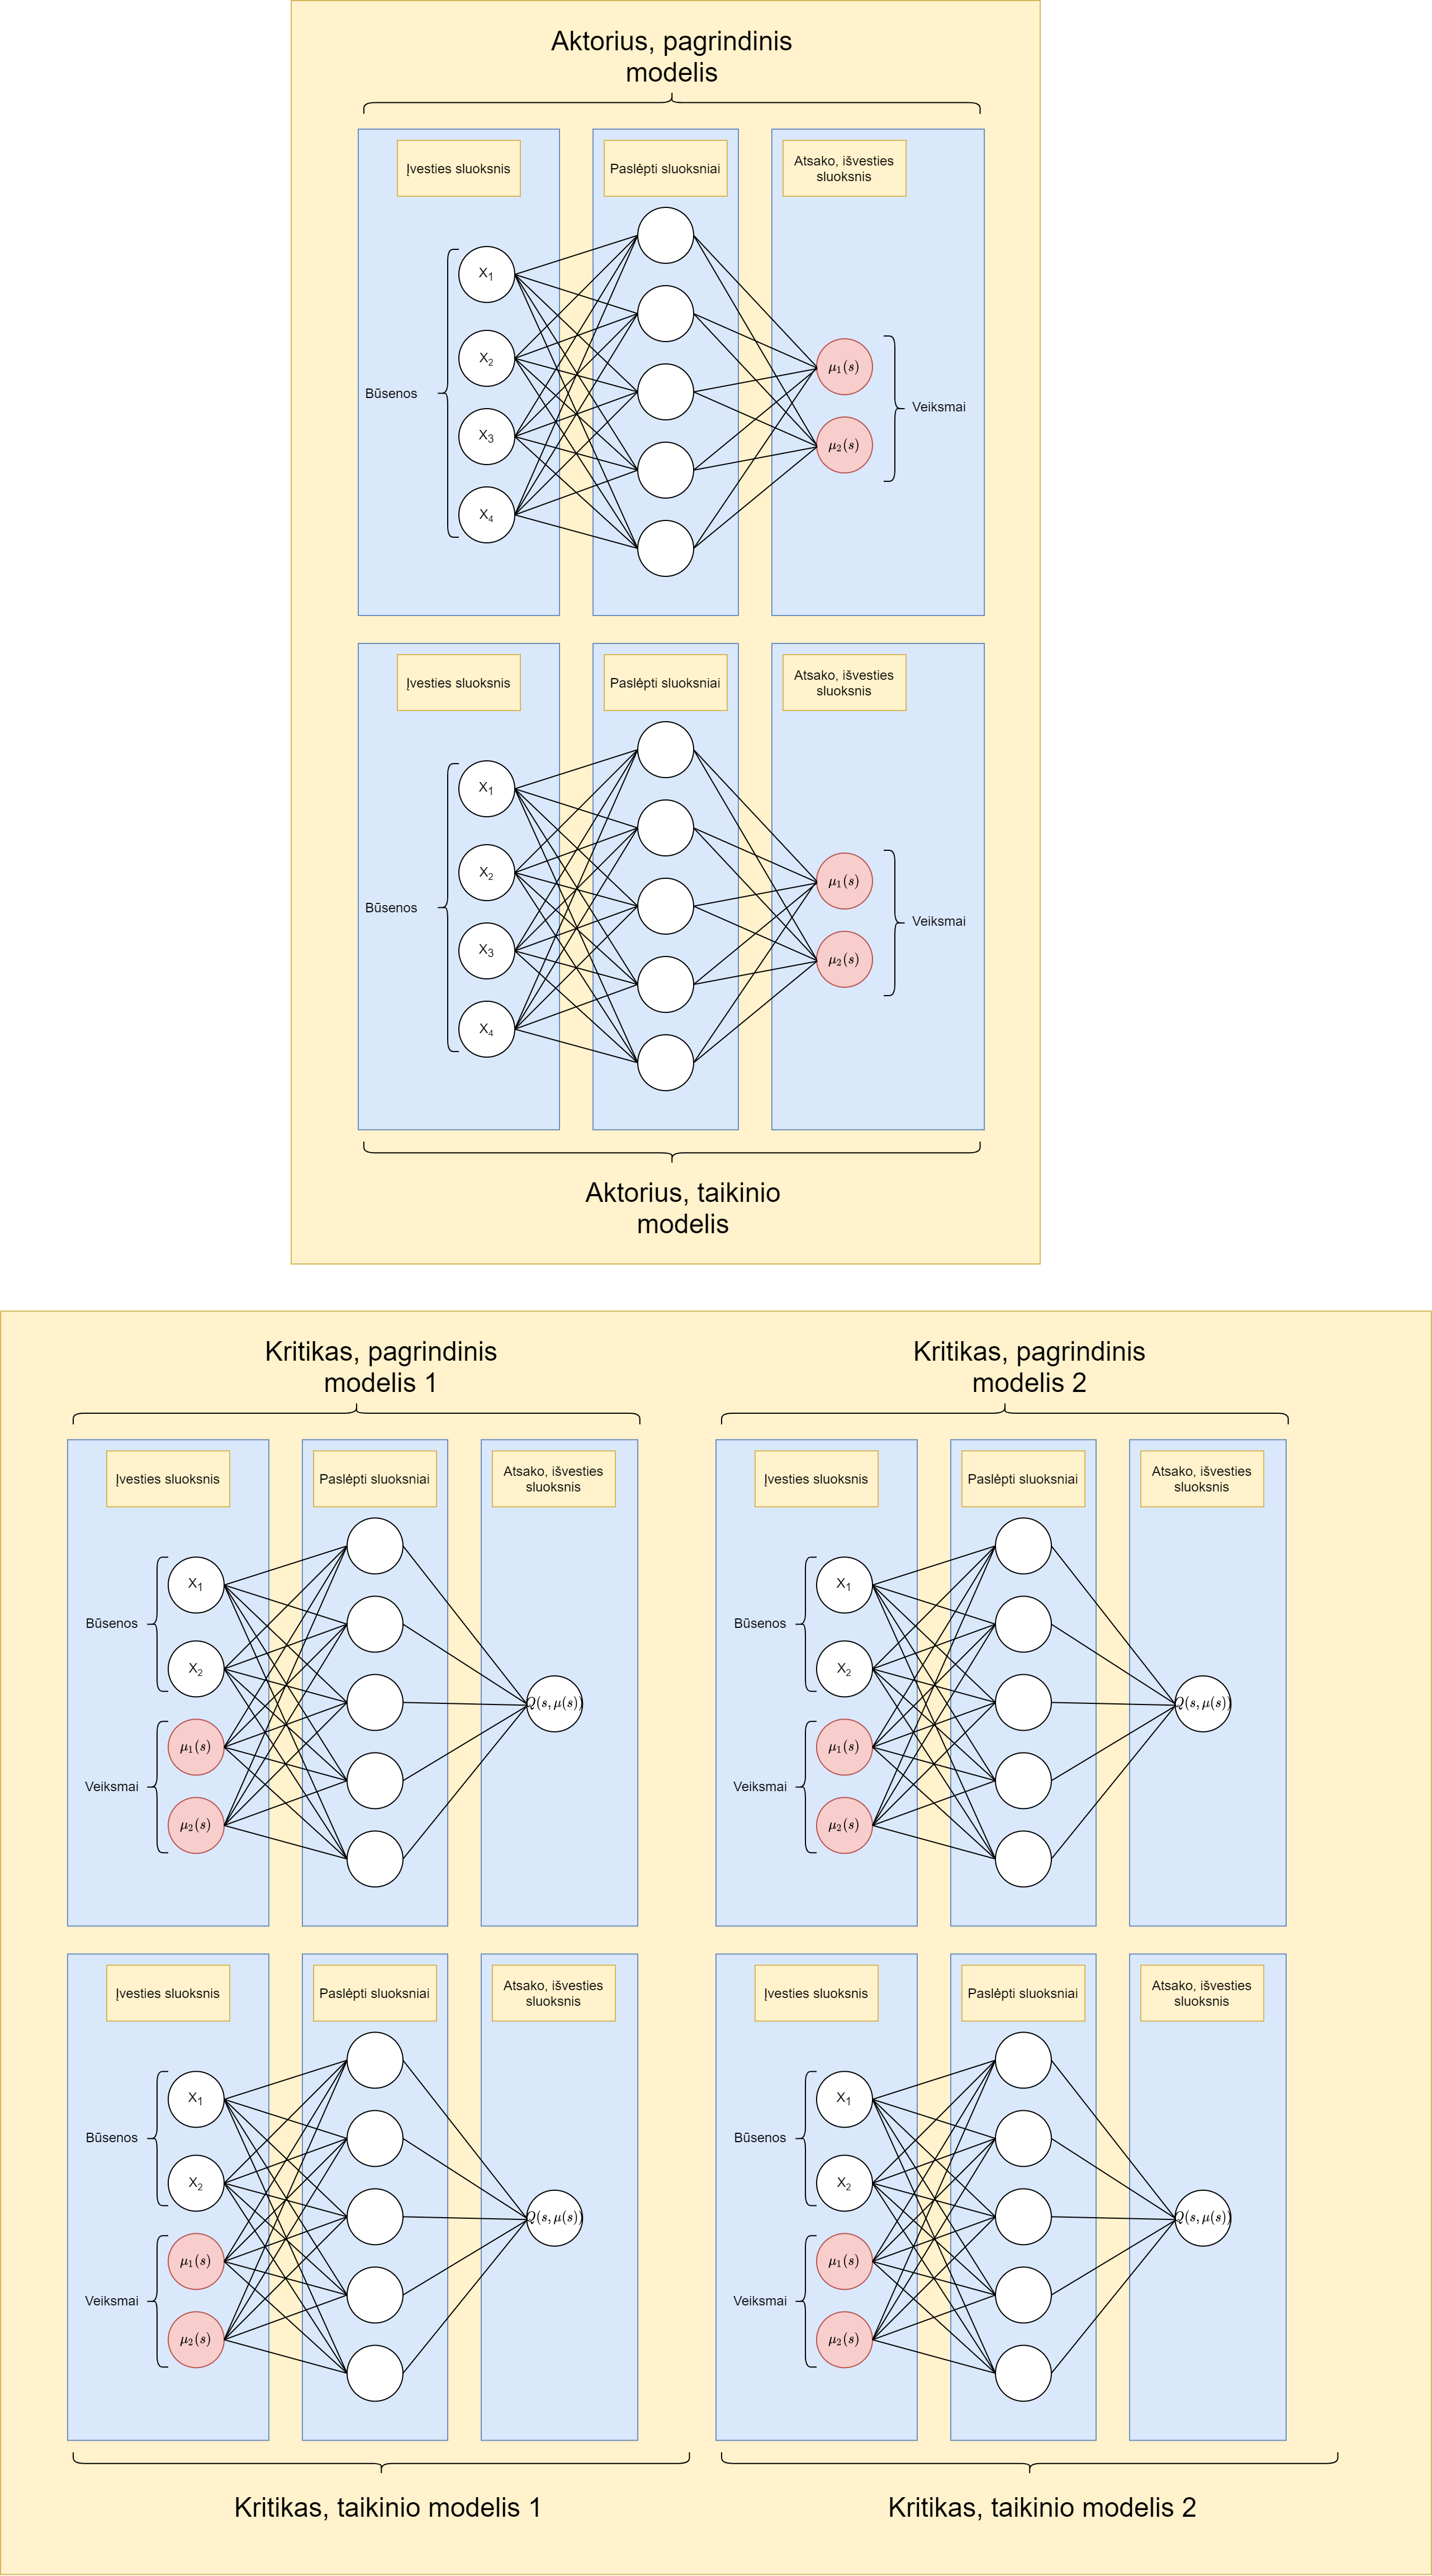
\includegraphics[width=.7\textwidth]{TD3}
\caption{TD3 modelio struktūra}
\label{TD3Struktura}
\end{figure}

\newpage

\section{Praktinė dalis}

Praktinėje dalyje bus įgyvendinamas TD3 metodas. Jo įgyvendinimui bus pasitelkta „Unity“ aplinka, kurioje egzistuos apmokamas agentas. Agentas yra keturių galūnių voras, kurio tikslas yra nuropoti į užsibrėžtą poziciją, judinant savo galūnes. Šis agento tikslas bei aplinka bus plėtojama pirmuosiuose praktinės dalies skyriuose. Toliau bus gilinamasi ties komunikacijos sluoksniu, kuriame simuliacijos aplinka bei mokymosi metodas TD3 keičiasi duomenimis. Kadangi TD3 metodas bus įgyvendintas „Python“ aplinkoje, o aplinkos simuliacija „Unity“ aplinkoje, šios dvi aplinkos negali vienas kitai persiųsti bei gauti duomenis. Todėl yra būtinas komunikacijos sluoksnis tarp šių dviejų aplinkų, padedančiu išsiųsti bei gauti žinutes. Galiausiai bus aptartas TD3 įgyvendinamas metodas bei jo rezultatai.

\subsection{Agentas, jo tikslai bei aplinka}

Per pastarąjį dešimtmeti skatinamieji metodai buvo pradėti taikyti įvairiuose srityse, tačiau viena iš sričių pasižymėjusiu didžiausiu proveržiu - robotų judėjimo kontroleriai. Roboto judėjimo užduotis tradiciniais metodais buvo ne vieną kartą stengiamasi išspręsti, bet rezultatai buvo nepatenkinami. Tačiau skatinamojo mokslo metodai pademonstravo, kad jie yra puikiai pritaikyti kontroliuoti agento galūnes, surasti optimalias judėjimo trajektorijas vedančias į užsibrėžto tikslo pasiekimą. Būtent šią užduoti ir įgyvendinsiu praktinėje dalyje. Bus pasitelktas „Unity“ aplinkoje sukurtas voras, kurio tikslas nuropoti iki specifinės koordinatės, kaip tai matome \ref{RLmodel} paveikslėlyje. Pagrindinis užduoties sunkumas kyla iš fizikinio judėjimo. Labai dažnai judėjimo agentai „Unity“ aplinkoje nejuda pagal fizikinius dėsnius, o paprasčiausiai animacijų pagalba jų judesiai yra įrašyti ir atkartojami. Tokios animacijos nėra paremtos fizika, kiekviena agento galūnė kiekvieno kadro metu įgyja įrašytas pozicijų koordinatės. Toks judėjimas neprisitaiko prie kintančios, dinaminės aplinkos ir roboto galūnės dažnai kerta objektus kiaurai. Šias problemas išsprendžia fizika paremtas galūnių judinimas, kurio programiškai iki šiol įgyvendinti buvo neįmanoma. Tik neseniai pasitelkus statistiniais mokymosi metodais kaip TD3 buvo pasiektas fizikinis agentų judėjimas.

Taigi kiekvieno epizodo metu voras yra sukuriamas aukštai ore. Jis turi sugebėti nusileisti ant savo galūnių bei nuropoti ties žaliu kubeliu. Sėkmingai jį pasiekus epizodas nesibaigę, yra sukuriamas naujas žalias kubelis, kurį voras vėl turi pasiekti. Šis būdas skatina vorą aplankyti naujas verčių būsenas susijusias su voro apsisukinėjimu. Epizodas baigiasi kuomet pasiekiamas epizodo maksimalų žingsnį, kurį galime traktuoti kaip laiko intervalą. Taip pat epizodas gali baigtis anksčiau, jei yra pasiekta terminuojanti būsena. Voro aplinkos atveju tai nutinka jei pagrindinė kūno dalis arba viršutiniai sąnariai pasiekę žemę. Kuo ilgiau voras išgyveną bei kuo arčiau jis yra žalio kubelio, tuo agentas gauna didesnį epizodo kaupiamąjį apdovanojimą. Tai ir yra agento pagrindinis tikslas, gauti kuo didesnį apdovanojimą. 

\subsection{Mokymosi seka}

Voro agento mokymosi procesas yra identiškas aptartiems mokymosi metodams ir sudarytas iš šių iteracinių žingsnių:

\begin{enumerate}
  \addtolength{\itemsep}{-0.5\baselineskip} 
  \item TD3 modelis turi dabartines voro būsenas. Turint šias būsenas TD3 pateikia naujus veiksmus.
  \item Voras gauną TD3 modelio pateiktą veiksmą bei jį atlieką.
  \item Atlikus veiksmą gaunama nauja būsena bei apdovanojimas. Šios vertės nusiunčiamos TD3 modeliui. 
  \item TD3 gavęs pateikto veiksmo rezultatą - naują būsena bei apdovanojimą, pradeda modelio apmokymą. Tai atlikus naujos būsenos tampa dabartinėmis ir pradedama naują iteracija. Dažniausiai apmokymas būna atidedamas ir jis įvyksta pasibaigus agento epizodui arba paralelizuotams agentams atlikus tam tikrą kiekį žingsnių.
\end{enumerate}


Svarbu pastebėti, kad apdovanojimų bei būsenų duomenys nusiunčiami TD3 modeliui ne kiekvieno simuliacijos kadro metu, o tik kas penkis „Unity“ fizikos simuliacijos žingsnius. Kitaip tariant agentui atlikus veiksmus jis laukia penkis „Unity“ fizikos atnaujinimus, per kuriuos jo galūnės pakeičią poziciją penkis kartus po labai maža atstumą. Tai atlikus agentas tik tada užfiksuoja naują įgytą būseną. Per šiuos penkis žingsnius jo apdovanojimas yra kaupiamas - kas žingsnį pridedame po apskaičiuota apdovanojimą. Šis penkių kadrų atnaujinimo atidėjimas padeda pasiekti ryškesni naujo veiksmo ir jo pasekmės ryšį. Taip pat tai sumažiną duomenų kiekį bei pagreitiną mokymą.

\subsection{Aplinka}

Voro aplinka susideda iš trijų elementų:
\begin{enumerate}
  \addtolength{\itemsep}{-0.5\baselineskip} 
  \item Voras.
  \item Tuščia, lygi arena, su keturiomis, areną apsupančioms, sienomis.
  \item Žalias kubelis, iki kurio vorui reikia nuropoti.
\end{enumerate}

Aplinkos atvaizdavimą matome \ref{arena} paveikslėlyje. Joje agentas praleidžia visą savo mokymosi laiką. Aplinka bei pats fizikiniais dėsniais paremtas voras yra jau sukurtas „Unity“ programuotojų. Jie pasitelkė skatinamojo mokslo PPO metodus apmokyti vorą ropoti bei pasiekė įspūdingus rezultatus. Mano mokymo metu bus naudojamas TD3 metodas, kuris yra specifiškai pritaikytas deterministiniams veiksmams bei panašiuose užduotyse dažniau pasiekia optimalesnius rezultatus. 

\begin{figure}[h!]
\centering
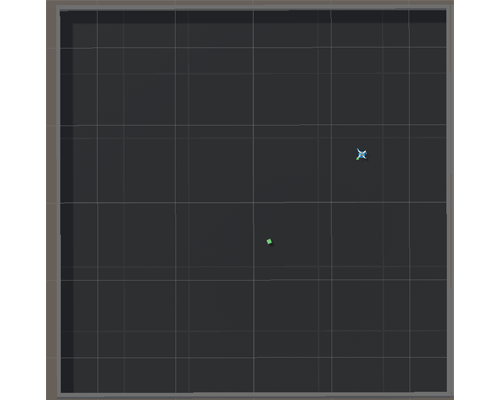
\includegraphics[width=.7\textwidth]{arena}
\caption{Voro aplinka}
\label{arena}
\end{figure}

Arena įgijo šį specifini išsidėstymą, dėl šių tolimesnių priežasčių:

\begin{enumerate}
  \addtolength{\itemsep}{-0.5\baselineskip} 
  \item Arena lengva padvigubinti, sukurti daugybe jos kopijų. Tai naudinga paraleliam mokymuisi, kuris bus aptartas tolimesniuose skyriuose.
  \item Lygioje arenoje, be įdubimu bei iškilimu, yra lengviau apmokyti agentą. Nereikia programuoti sudėtingų metodų įdubimams aptikti bei informuoti agentą apie jų egzistavimą. Tai sumažina būsenų erdvę.
  \item Žalias kubelis, iki kurio vorui reikia nuropoti. Tai yra paprasčiausias atskaitos taškas, naudojamas įvertinti agento optimalumą.
  \item Keturios sienos, neleidžiančio vorui nukristi už simuliacijos ribų.
\end{enumerate}

Taigi ši arena yra paprasčiausia įmanoma aplinka, kuri padeda įsitikinti mokymosi metodo efektyvumu. Jei pasirinktas mokymosi metodas sugeba susidoroti su šia aplinka, ją galima pradėti palaipsniui sunkinti bei pritaikyti savo reikmėms.

\subsection{Duomenys}

Kaip matome \ref{TD3Struktura} paveikslėlyje, TD3 mokymosi metodų neuroninių tinklų įvestis yra būsenų erdvė bei aproksimuoti veiksmai. Tuo tarpu pagrindinė išvestis yra veiksmų taisyklės - kokius tolimesnius veiksmus turėtų atlikti agentas. Šias veiksmų reikšmes padeda apskaičiuoti apdovanojimai, taip pat viena iš įvesčių reikšmių, apskaičiuojanti taikinio reikšmes, kurias neuroninis tinklas turėtų aproksimuoti. Taigi toliau visi šie duomenys bus aptariami detaliau.

\subsubsection{Įvestis - būsenos}

Tiek aktoriaus modelis, aproksimuojantis veiksmų taisykles, tiek kritiko modelis, aproksimuojantis būsenų vertes, priima būsenų reikšmes. Voro būsenų reikšmės susideda iš 127 reikšmių. Jas galima suskaldyti į šias kategorijas:

\begin{enumerate}
  \addtolength{\itemsep}{-0.5\baselineskip} 
  \item Voro galūnės. Kiekviena voro koja susideda iš dviejų sąnarių: viršutinio bei apatinio sąnario.
  \item Voro pagrindinis kūnas. Viršutiniai voro sąnariai susijungia su šia dalimi.
\end{enumerate}

Kaip matomo \ref{VoroGalunes} paveikslėlyje apatinis sąnarys kontroliuoja koją, užtušuota rausvai. Viršutinis sąnarys kontroliuoja koją užtušuota oranžine spalva. Ir galiausiai visi viršutiniai sąnariai susijungia į pagrindinę kūno dalį užtušuota žalsvu atspalviu.

\begin{figure}[h!]
\centering

\includegraphics[width=.7\textwidth]{VoroGalunes}
\caption{Voro galūnės}
\label{VoroGalunes}
\end{figure}

Visos voro galūnės kaupia ne konkrečią informaciją, bet santykinę. Kitaip tariant nėra kaupiama tiksli voro pozicija, bet atstumo vektorius nuo voro iki taikinio, žalio kubelio. Tokiu būdu voras neprisitaiko prie konkrečios aplinkos, agentas gali lengvai ropoti įvairiose arenose. Tai ypatingai svarbu paralelizuojant mokymosi procesą. Taigi visi sąnariai kaupia šias būsenas:

\begin{enumerate}
  \addtolength{\itemsep}{-0.5\baselineskip} 
  \item Ar galūnė liečia žemės paviršių. Priklausomai nuo to ar liečia, simuliacija gali būti nutraukiama ir įvardijama kaip nepasisekusi. Ši sąlyga galioja viršutiniam sąnariui, kadangi nenorime, kad jis liestų žemę, jis nuolatos turi būti virš jos.
  \item Atstumo vektorius tarp sąnario greičio vektoriaus bei agento-kubelio atstumo vektoriaus. Mes norime, kad atstumas būtų lygus nuliui, kitaip tariant abu vektoriai žiūri į tą pačią trajektoriją.
  \item Laipsnių atstumas tarp sąnario pozicijos vektoriaus bei atstumo vektoriaus tarp agento bei kubelio. Turi panašumų su praeitu punktu, tačiau duomenys išreikšti laipsniais.
\end{enumerate}

Pagrindinė kūno dalis kaupia šią informaciją:
\begin{enumerate}
  \addtolength{\itemsep}{-0.5\baselineskip} 
  \item Ar liečia žemės paviršių. Jei taip, simuliacija yra nutraukiama.
  \item Pagrindinės kūno dalies atstumas iki žemės paviršiaus. Kadangi agentas turi sugebėti stovėti su savo kojomis ant žemės paviršiaus, voras turi žinoti kaip arti jis yra iki žemės.
  \item Atstumo bei laipsnių vektoriai, gaunami tokiu pat principu kaip sąnariuose.
\end{enumerate}

Taip pat kaupiamas vidutinis agento galūnių greitis. Kuo didesnis greitis, tuo jis gauna didesnį apdovanojimą. Tokiu būdu mes skatiname agentą judėti sparčiai.

Šios visos būsenos supakuojamos į vieną realiųjų skaičių masyvą ir nusiunčiamos TD3 mokymosi modeliui. Taip pat nusiunčiame apdovanojimą, kuris yra apskaičiuojamas „Unity“ aplinkoje.

\subsubsection{Apdovanojimas}

Duomenų talpykloje kaupiamos ne tik būsenos bet ir apdovanojimai. Jie atkeliauja iš „Unity“ aplinkos. Vorui atlikus TD3 modelio pateiktus veiksmus, jis apskaičiuoją atliktų veiksmų naudą. Vadovaujantis \ref{apdovanojimoPatarimas} skyriaus svarbiu patarimu, mes turime suformuoti apdovanojimo funkciją taip, kad jį neformuotų užduoties sprendimo būdo, o tik apdovanotų už pasiektą tikslą. Todėl apdovanojimo funkcija susideda iš šių trijų funkcijų:

\begin{enumerate}
  \addtolength{\itemsep}{-0.5\baselineskip} 
  \item Skaliarinė sandauga tarp pagrindinės kūno dalies greičio vektoriaus bei normalizuoto krypties vektoriaus nuo pagrindinio kūno į žalią kubelį. Šie vektoriai pavaizduoti \ref{voroGreicioVektoriai} paveikslėlyje, tačiau pateiktas žalias vektorius nėra vizualiai normalizuotas. Jei šie vektoriai sutampa, mes gauname vieneto vertę, žyminčią didžiausią įmanomą apdovanojimą. Tokiu būdu mes nurodome agentui judėti link žalio kubelio, bet nepasakome kaip konkrečiai atlikti šią užduoti.
  \item Skaliarinė sandauga tarp agento krypties vektoriaus bei normalizuoto krypties vektoriaus nuo pagrindinio kūno į žalią kubelį. Kitaip tariant jei agentas yra atsisukęs į žalią kubelį, jis gauną maksimalų apdovanojimą - vienetą.
  \item Apskaičiuojame ar vidutinis visų galūnių greitis atitinka mūsų pateiktą maksimalų greitį. Jei atitinką, priskiriame papildoma vieneto apdovanojimą, jei visai nesutampa, apdovanojimas tampa nulis. Tarpinės reikšmes pateikę sigmoido funkcija. Ši apdovanojimo funkcija buvo pridėta vėliausiai iš visų apdovanojimo funkcijų, kuomet buvo pastebėtas voro lėtas slinkimas į žaliąjį kubelį. Agentas išmokęs stabiliai stovėti ant kojų ir iš lėto ropoti link žaliojo kubelio po truputi pastebi, kad kuo greičiau juda, tuo didesnį pasiekę apdovanojimą. 
\end{enumerate}

Šie apdovanojimai, kiekvienos fizikos atnaujinimo metu yra apskaičiuojami bei sudedami į vieną kaupiamąjį apdovanojimą. Jis, kartu su būsenomis, nusiunčiamas TD3 modeliui. Nusiuntus apdovanojimą jis tampa nuliu ir jo skaičiavimo procesas prasideda iš naujo.

Kiekvieno epizodo metu mes kaupiame epizodo galutinį apdovanojimą. Jis slenkančio vidurkio metodu apskaičiuoja paskutinių penkiasdešimties epizodų apdovanojimo vidurkį. Šis kiekvieno epizodo metu kintantis matas yra pagrindinis kriterijus pagal kurį vizualiai vertiname modelio efektyvumą. Mokymuisi vykstant jis turi kilti. Tai parodo vis didėjanti epizodų apdovanojimą.

\subsubsection{Išvestis - veiksmai}

TD3 aktoriaus neuroninis tinklas priėmęs būsenas išveda veiksmus. Iš viso yra apskaičiuojami dvidešimt veiksmo verčių, kuriuos voras gauną. Šios veiksmų vertės kontroliuoja voro viršutines bei apatines galūnes. Toliau bus vardijama galūnių veiksmų vertės:

\begin{enumerate}
  \addtolength{\itemsep}{-0.5\baselineskip} 
  \item Viršutinis voro sąnarys gali sukinėtis aplink x bei y koordinačių ašį, tačiau ne z, kaip tai matome \ref{SanarioJudejimoTrajektorijos} paveikslėlyje. Veiksmų vertės nurodo galutinę šio sąnario poziciją laipsniais bei kiek jėgos bus suteikta šiai pozicijai pasiekti.
  \item Apatinio sąnario veiksmų vertės yra identiškos, tačiau šis sąnarys gali sukiotis tik aplink x ašį.
\end{enumerate}

Kadangi TD3 aktoriaus neuroninio tinklo išvestis yra tanh funkcija, mes nuolatos turime konvertuoti $[-1,1]$ intervalo reikšmes į konkrečias laipsnių bei jėgų reikšmes. Taigi agentas gauna naujas galūnių judėjimo reikšmes ir tokiu būdu jis jas po truputi krutina.

\begin{figure}[h]
\centering

\includegraphics[width=0.5\textwidth]{SanarioJudejimoTrajektorijos}
\caption{Viršutinio sąnario judėjimo trajektorijos}
\label{SanarioJudejimoTrajektorijos}
\end{figure}


\subsection{Komunikacijos sluoksnis}

TD3 modelis bei voro aplinka yra įgyvendinta skirtinguose programose. Voro aplinka yra įgyvendinta „Unity“ programoje, o TD3 modelis „Python“ aplinkoje. Kadangi „Unity“ variklis negali kompiliuoti „Python“ kodo, teko įgyvendinti šias dvi aplinkas atskirose programose. Tai sukėlė pastovių keblumų, kadangi duomenys tarp šių dviejų programų turi nuolatos bei užtikrintai keistis, kas dažnai neįvykdavo. Taigi buvo sukurtas komunikacinis sluoksnis, kuris užtikrindavo pastovų žinučių siuntimą iš TD3 modelio į „Unity“ agento aplinką. TD3 atliko serverio rolę, nuolatos pirmutinis siusdavo duomenis agento aplinkai bei iš jo laukdavo atsakymo. Žinutėms siųsti buvo pasirinktas json formatas dėl dviejų priežasčių: abi skirtingos aplinkos turi json nuskaitymo bibliotekas bei į json lengva įrašyti norimą informaciją. 

Buvo įgyvendintos dvi esminės žinutės: naujo epizodo bei duomenų rinkimo. Šios dvi žinutės pasižymi panašia duomenų forma - išsaugome tekstinę komandą bei pridedame norimus duomenis. Toliau pateiktos dvi skirtingos siunčiamos komandos:

\begin{enumerate}
  \addtolength{\itemsep}{-0.5\baselineskip} 
  \item Naujo epizodo komanda. Serveris praneša agentui reikalavimą pradėti naują epizodą. Jį gavęs agentas inicializuoja vorą į pradinę epizodo poziciją ir išsiunčią būsenos duomenis į serverį. Serveris gavęs šiuos duomenis gali pradėti mokymosi procesą.
  \item TD3 gavęs voro būsenas aproksimuoją naują veiksmą bei nurodo serveriui išsiųsti jį agentui. Voras gavęs veiksmus juos atlieka. Juos atlikęs atgal išsiunčią serveriui naujai įgytas būsenas, apdovanojimą bei ar ši nauja būsena terminuoją epizodą.
\end{enumerate}

Šis duomenų keitinėjimasis pateiktas \ref{Reset} paveikslėlyje.

\begin{figure}[h]
\centering
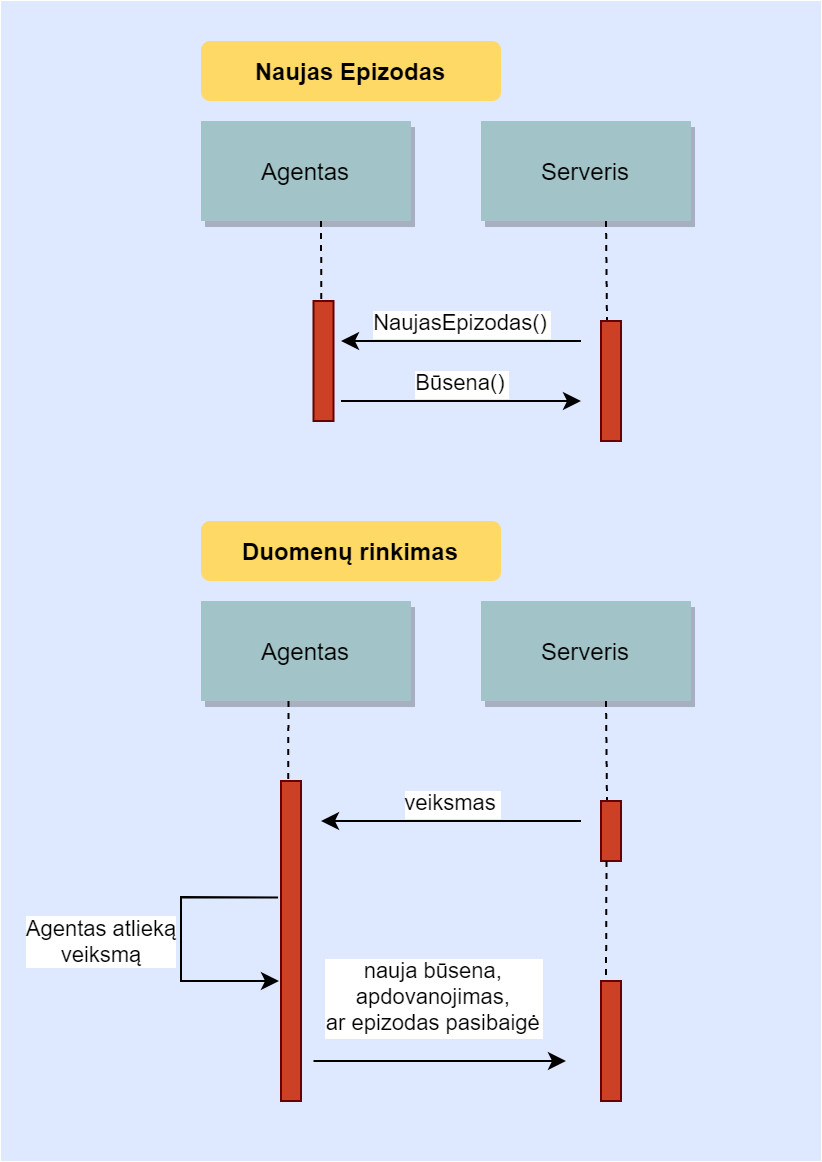
\includegraphics[width=0.7\textwidth]{Reset}
\caption{Serverio bei agento komunikavimo sluoksnis}
\label{Reset}
\end{figure}

\subsection{Mokymosi procesas}

Vienas didžiausių skatinamojo mokslo trūkumų yra labai lėtas mokymosi procesas, reikalaujantis daug resursų. Su šia problema buvo susidurta vos ne iš anksto. Pradžioje įgyvendinant TD3 modelį duomenys į patirčių talpyklą buvo renkami tik iš vieno agento. Nors modelio vidutinis apdovanojimų kiekis po truputi didėjo, tačiau tai buvo lėtas procesas. Net vienai mokymo dienai praėjus, voras sugebėdavo išmokti tik stovėti ant savo keturių galūnių bei nedemonstruodavo jokio progreso ties ropojimu į žalio kubelio poziciją. Todėl buvo pasitelktas paralelinis mokymasis, kuris sparčiai pagreitino mokymosi procesą. Vietoj vienos aplinkos, buvo sukurtos dešimt identiškų aplinkų. Sukurtų aplinkų vorų mokymosi seka išliko tokia pati, buvo apmokamas vienas modelis. Tačiau šį karta patirčių talpykla buvo pildoma ne vieno agento pagalba bet dešimties. Ši technika paspartina mokymosi procesą iki dešimties kartų. 

Taip pat buvo pritaikytas simuliacijos spartinimas. „Unity“ variklyje kiekvienas fizikinis kadras užtrunka 0.2 ms. Norint pasiekti greitesnį agentų simuliavimo greitį, ši vertė buvo pakeista į 0.01333 ms. Kitaip tariant įvykdavo daugiau fizikinių atnaujinimų, dažniau pakisdavo vorų galūnių pozicijos. Tokiu būdu paspartinus simuliaciją, vizualiai agentai vos ne dvigubai greičiau atlikinėdavo savo veiksmus. 

Tačiau net su įvardintais mokymosi pagreitinimais, mokymosi procesas ilgai užtrukdavo. Galutinis voro modelis buvo apmokamas vos ne dvi dienas. Šis ilgo mokymosi didžiausias trūkumas yra lėtas modelio iteravimas. Pakeitus pora modelio parametrų, rezultatų reikia vėl iš naujo laukti pora dienų.

\subsection{TD3 modelio įgyvendinimas}

Nors buvo planuojama sudaryti TD3 modelį naudojantis savo įgyvendintais neuroniniais tinklais, tačiau pastebėjus lėta mokymosi procesą ši idėja buvo atšaukta. Buvo pasitelkti Tensorflow bibliotekos sukurti neuroniai tinklai, kurių pagrindinis privalumas yra gebėjimas atlikti matricines operacijas paralelizuotai bei vaizdo plokštėje, paspartinant skaičiavimus, o ne procesoriuje. Norint įgyvendinti šiuos du punktus, jie reikalauja nepaprastai daug žinių ir laiko, todėl TD3 modelio verčių bei veiksmų taisyklių aproksimacijos yra įgyvendintos Tensorflow neuroninių tinklų pagalba. Taip pat vienas didžiausių privalumu naudojantis Tensorflow neuroniais tinklais, yra tai kad TD3 yra paplitęs metodas ir jo įgyvendinimo procesą galima lengvai surasti bei perprasti. Vienas iš susidurtų didžiausių sunkumų buvo veiksmo taisyklių neuroninio tinklo parametrų gradiento radimas, kaip matome \ref{keistasGradientas} formulėje. Šis gradientas apima dviejų neuroninių tinklų gradientą, kurio apskaičiavimas pasirodė keblus. Iki šiol gradientinis nuolydis buvo atliekamas tik vieno neuroninio tinklo parametrams. Tačiau pateiktoje formulėje gradientas keliauja per du neuroninius tinklus. Įsigilinus į \ref{netoksKeistasGradientas} formulę, galime pastebėti paprastą gradiento formą: kaip gautos veiksmo taisyklių reikšmės, keičia \ref{netoksKeistasGradientas} formulę. Norint atsakyti į šį klausymą pradžioje reikia surasti vieno iš pasirinkto pagrindinio kritiko modelio įvesties neuronų veiksmų išvestines, pavaizduoto raudonai \ref{TD3Struktura} paveikslėlyje, bei jas sudauginti su aktoriaus paprastu neuroniniu gradientiniu nuolydžiu. Tokiu būdu optimizuojame aktoriaus pagrindinio neuroninio tinklo parametrus. Tuo tarpu kritiko modelio optimizavimas yra identiškas giliojo-Q metodui, aptartam \ref{GilusisQSkyrius} skyriuje.

\subsection{Rezultatai}


Voro mokymasis truko porą dienų ir mokymuisi pasibaigus agentas gebėdavo dideliu greičiu ropoti link žaliojo kubelio. Mokymosi proceso gerumo kriterijus buvo vidutinis judantis apdovanojimas, kuris pateiktas \ref{apdovanojimuGrafikas} paveikslėlyje. Viršutinė ašis žymi vieno epizodo vidutinį judanti apdovanojimą, o apatinė ašis žingsnių kiekį.

\begin{figure}[h]
\centering
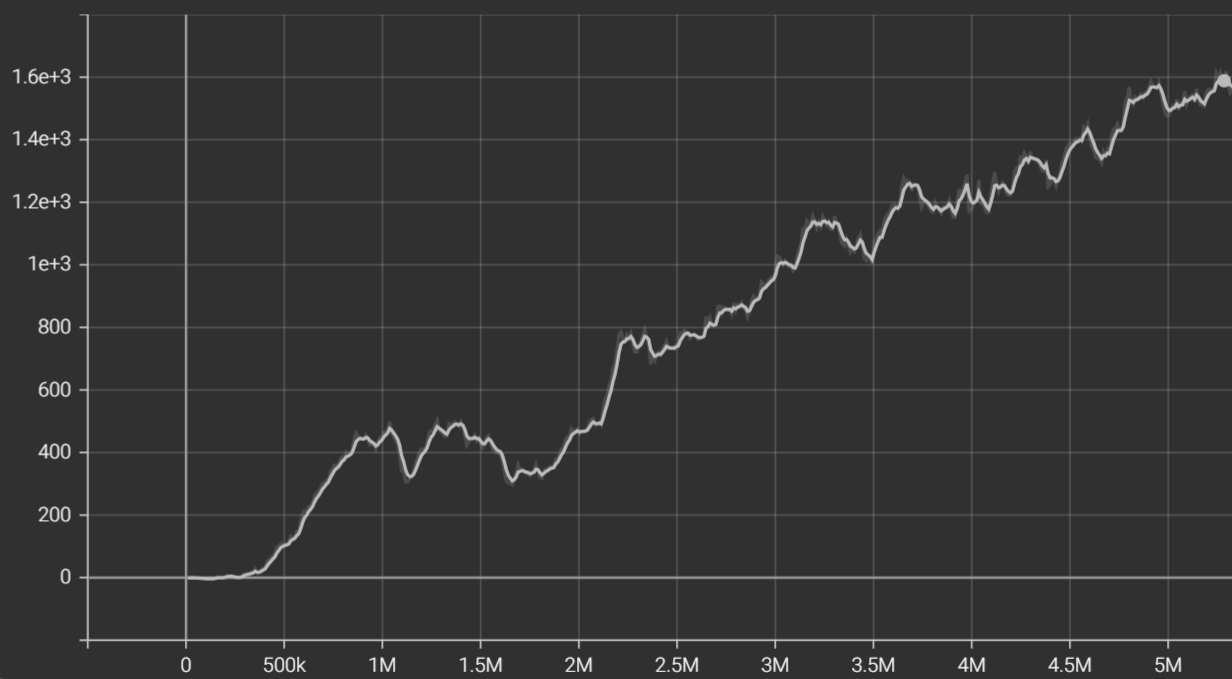
\includegraphics[width=1\textwidth]{apdovanojimuGrafikas}
\caption{Apdovanojimų grafikas}
\label{apdovanojimuGrafikas}
\end{figure}


Agentui besimokant buvo pastebėti šie mokymosi etapai:
\begin{enumerate}
  \addtolength{\itemsep}{-0.5\baselineskip} 
  \item Nuo 0 iki 500 tūkst. žingsnio agentas išmoko stovėti ant keturių kojų.
  \item Nuo 500 tūkst. iki 1.5 mln. žingsnio agentas išmoko judėti link žaliojo kubelio. Ties 1.2 mln. žingsniu matome smarku pagrindinio rodiklio kritimą, susijusi su katastrofinio užmiršimo problema. Ši problema atsiranda, kuomet senos patirčių talpyklos reikšmės yra pakeičiamos naujomis, agentas užmiršta optimalias strategijas. Kadangi mano talpyklos dydis yra 1 mln. reikšmių, netrukus šis katastrofinis užmiršimas pasireiškė. Tačiau tai buvo trumpalaikis efektas bei agentas sugebėjo toliau tobulėti.
  \item Ties 2 mln. žingsniu agentas išmoko efektyviau sukiotis ir užtikrinčiau stovėti ant savo keturių galūnių. Voras rečiau gaudavo baudą už nukritimą ant pagrindinės kūno dalies.
  \item Nuo 2.5 mln. žingsnio agento greičio apdovanojimo funkcija pradėjo įgyti didžiulę įtaką. Agentas pastebėjo, kad kuo greičiau jis juda, tuo didesnį nuopelną gauną. Tai privedė ties greitu galūnių klibinimu.
  \item Ties 5 mln. žingsniu voras įgijo optimalų judėjimą. Pasiekus žalią kubelį voras staigiai apsisukdavo bei greitai nuropodavo link naujo kubelio. Taip pat pastebėtas įdomus stabdymo bruožas. Agentui priartėjus prie žalio kubelio, jis smarkiai pradeda stabdyti, mažindamas susidariusi momentinį greitį. Pasiekus žalią kubelį bei esant vos ne stovinčioje pozicijoje, jis gali žymiai greičiau atsisukti į kubelio trajektoriją ir vėl pradėti ropoti link jo.
\end{enumerate}

Taigi TD3 modelis sugebėjo sėkmingai apmokyti vorą judinti fizikines galūnes bei užtikrintai pasiekti žaliąjį kubelį.

\newpage
\section{Išvados}

Atlikus skatinamųjų modelių analizę, gautos išvados:

\begin{enumerate}
  \addtolength{\itemsep}{-0.5\baselineskip} 
  \item Neuroninis tinklas yra efektyvus įrankis aproksimuoti skatinamuosius modelius. Tačiau neuroniniai tinklai yra labai nestabilūs, prasta jų inicializacija priveda prie prastos konvergacijos. Svarbu teisingai priskirti neuroninio tinklo parametrus, pritaikyti reguliarizacijas, neužmiršti gradientinio nuolydžio momentinius algoritmus kaip Adam. Pagal šiuos principus buvau sukūręs savo neuroninius tinklus, tačiau dėl lėtos konvergacijos buvo pasitelkta Tensorflow neuroninių tinklų biblioteka.
  \item Ne generalizuoti skatinamieji modeliai yra prasti metodai. Šie metodai gali būti pritaikomi tik mažos dimensijos problemose. Kylant būsenų dimensijai, konvergavimo laikas greitai pakyla į begalines reikšmes. Todėl skatinamieji metodai dešimtmečius po jų atradimo buvo retai pritaikomi. Dažniausiai šie metodai buvo pritaikomi plėtoti skatinamąjį mokslą demonstruojant jų efektyvumą primityviuose pavyzdžiuose. Buvo įgyvendinti SARSA, Q-mokymosi metodai, kurie gali optimizuoti tik mažos būsenų erdvės uždavinius.
  \item Aproksimuojami bei generalizuojami skatinamieji metodai transformavo nepopuliarų mokslą į turinti didžiulio potencialo. Atradus veiksmo taisyklių gradientą, neuronų tinklais aproksimuojami skatinamieji metodai išsprendė didžiausią šio mokslo problemą - aukštų dimensijų aproksimavimas. 
  \item Pritaikytas giliojo-Q mokymosi metodas pasižymi tik būsenos verčių aproksimavimu, neturi veiksmo taisyklių aproksimizacijos. Jis yra silpniausias iš visų aproksimuojamų skatinamųjų modelių, tačiau vienas iš įtakingiausių. Iš jo kilo daugybe metodų, kaip PPO, DPG, DDPG, TD3.
  \item Buvo įgyvendintas TD3 metodas, kuris sugeba pateikti deterministines veiksmo taisykles. Metodas buvo sėkmingai pritaikytas spręsti voro fizikinę judėjimo problemą. Apmokytas metodas sugebėjo tiksliai pateikti optimalius veiksmus voro galūnėms, kuriomis voras ropojo iki nusibrėžtos pozicijos.
\end{enumerate}


%\subsection{TODO}
%-pakeist * i \cdot
%-prideti priedus - koda
%





\newpage
% ---------------------------------------------------------------- LITERATŪRA --
\phantomsection
\addcontentsline{toc}{section}{Literatūra}

% Bibliografija nėra įprastas skyrius, todėl į LaTeX dokumento turinį neįtraukiama. 
% Norint, kad bibliografija būtų įtraukiama į turinį, tenka sukurti fiktyvų skyrių 
% ir nurodyti, kaip jis bus atvaizduojamas turinyje.

\begin{thebibliography}{99}

\bibitem{TDSutton} 
Sutton, R. \& Barto, A. 1987, ‘A Temporal-Difference Model of Classical Conditioning’, in Proceedings of the Ninth Annual Conference of the Cognitive Science Society, Seattle, WA, pp. 355–78.\href{http://incompleteideas.net/papers/sutton-barto-TD-87.pdf}{PDF}.

\bibitem{Pavlov} 
Ivan P. Pavlov(1927). CONDITIONED REFLEXES: AN INVESTIGATION OF THE PHYSIOLOGICAL ACTIVITY OF THE CEREBRAL CORTEX \href{http://psychclassics.yorku.ca/Pavlov/lecture6.htm}{html}.

\bibitem{Adam}
Diederik P. Kingma, Jimmy Lei Ba (2015). ADAM: A METHOD FOR STOCHASTIC OPTIMIZATION
\href{https://arxiv.org/pdf/1412.6980.pdf}{PDF}


\bibitem{QLearning}
Watkins, C.J.C.H. (1989). Learning from Delayed Rewards. \href{https://www.cs.rhul.ac.uk/~chrisw/new_thesis.pdf}{PDF}

\bibitem{DeepQLearning}
 Methods and Apparatus for Reinforcement Learning, US Patent \#20150100530A1. US Patent Office. 9 April 2015. Retrieved 28 July 2018. \href{https://patentimages.storage.googleapis.com/71/91/4a/c5cf4ffa56f705/US20150100530A1.pdf}{PDF}

\bibitem{AtariGoogle}
Volodymyr Mnih, Koray Kavukcuoglu, David Silver, Alex Graves, Ioannis Antonoglou, Daan Wierstra, Martin Riedmiller (2013). Playing Atari with Deep Reinforcement Learning. \href{https://arxiv.org/pdf/1312.5602v1.pdf}{PDF}

\bibitem{GoogleDeepQLearning}
Volodymyr Mnih, Koray Kavukcuoglu, David Silver (2015). Human-level control through deep reinforcement learning \href{https://storage.googleapis.com/deepmind-media/dqn/DQNNaturePaper.pdf}{PDF}

\bibitem{DPG}
David Silver, Guy Lever, Nicolas Heess, Thomas Degris, Daan Wierstra (2014). Deterministic Policy
Gradient Algorithms. ICML, Jun 2014, Beijing, China. ffhal-00938992f \href{https://hal.inria.fr/file/index/docid/938992/filename/dpg-icml2014.pdf}{PDF}

\bibitem{DDPG}
Timothy P. Lillicrap, Jonathan J. Hunt, Alexander Pritzel, Nicolas Heess,Tom Erez, Yuval Tassa, David Silver \& Daan Wierstra (2016). CONTINUOUS CONTROL WITH DEEP REINFORCEMENT LEARNING. Google Deepmind London, UK
\href{https://arxiv.org/pdf/1509.02971.pdf}{PDF}

\bibitem{TD3}
Scott Fujimoto, Herke van Hoof, David Meger (2018). Addressing Function Approximation Error in Actor-Critic Methods
\href{https://arxiv.org/pdf/1802.09477.pdf}{PDF}





\end{thebibliography}
%
%
\newpage
% ------------------------------------------------------------------- PRIEDAI --
\appendix
\section{Priedai}

Visą programos kodą bei įgyvendintą projektą galima surasti nurodytoje \href{https://github.com/PaulJanen/RF-Learning}{github} paskyroje.

\boldmath
\printnoidxglossaries
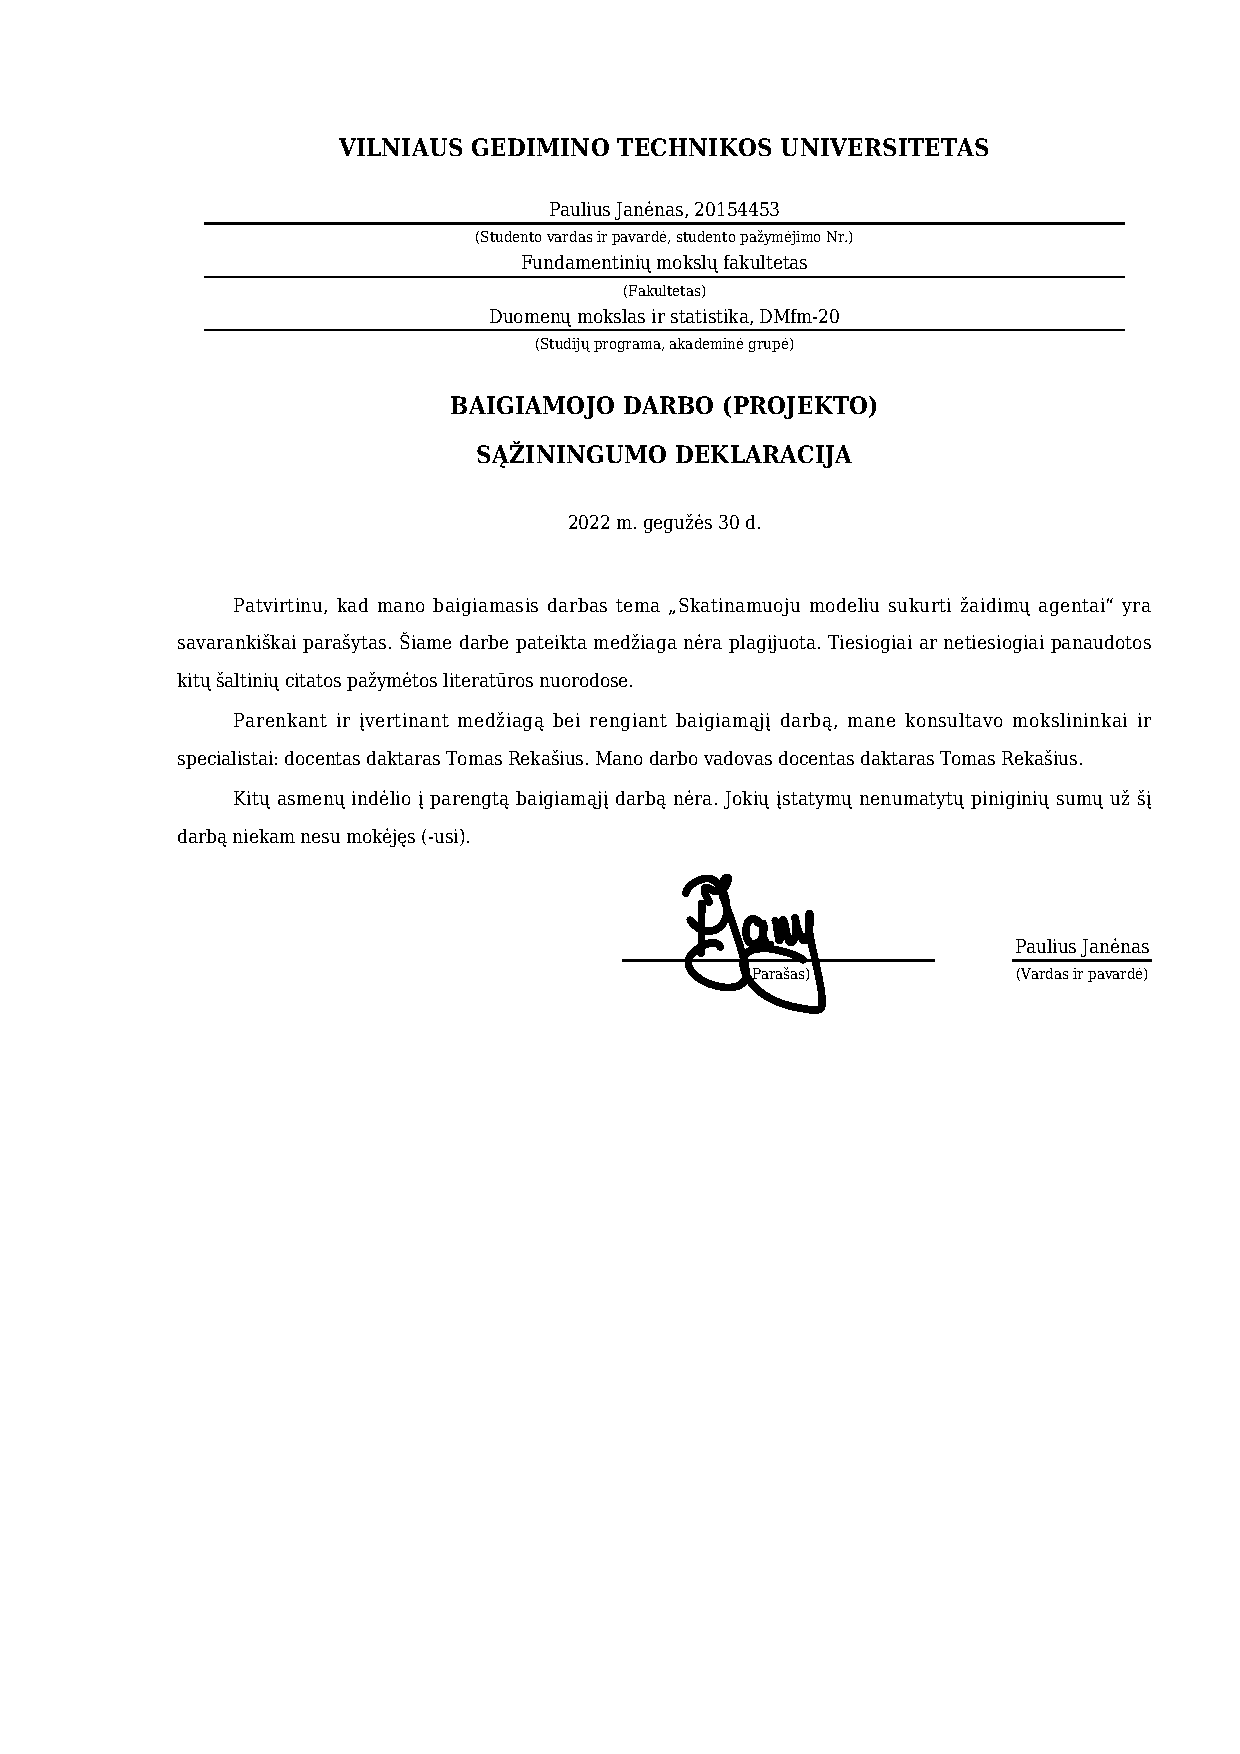
\includepdf[pages=-]{declaration_lt.pdf}






\end{document}
% ------------------------------------------------------------------------------
%  DOKUMENTO PABAIGA
% ------------------------------------------------------------------------------





